%% -*- coding: euc-jp -*-
%%
%% Master's Thesis
%%
%% Author: Yasunori Yusa
%%
\documentclass[12pt, a4j, twoside, openany, titlepage]{jsbook}
%
%% hyperref: EUC-JP -> Unicode
\usepackage{atbegshi}
\AtBeginShipoutFirst{\special{pdf:tounicode EUC-UCS2}}
%
%% packages
\usepackage{amsmath}  % AMS math extension
\usepackage{amssymb}  % AMS symbol extension
\usepackage{graphicx} % figure extension
\usepackage[margin=30truemm]{geometry} % geometry
\usepackage[nohints]{minitoc}
% \usepackage[nottoc]{tocbibind} % ToC of LoF and LoT
\usepackage{fancyhdr} % head and foot
\usepackage[dvipdfmx, bookmarks=true, bookmarksnumbered=true, pdfborder={0 0 0},
pdftitle={分離反復連成解法による大規模破壊力学シミュレーション},
pdfauthor={遊佐泰紀},
pdfsubject={Large-scale Fracture Mechanics Simulation Using Partitioned Iterative Coupling Algorithm},
pdfkeywords={数値計算, 計算破壊力学, 大規模有限要素法, 連成解析, 反復法}]{hyperref} % hyperref
\usepackage{url}         % URL
\usepackage{cite}        % cite references
\usepackage{algorithmic} % algorithm
\usepackage{mymath}      % my math package
%
%% fonts
\usepackage{pxfonts}  % PX (Palatino)
\usepackage{palatino} % Palatino
\usepackage{bfutura}  % Futura
\usepackage{courier}  % Courier
%
%% line space optimized for 30 lines
\renewcommand{\baselinestretch}{1.18}
%
%% ToC of subsubsections
\setcounter{secnumdepth}{3}
\setcounter{tocdepth}{3}
\setcounter{minitocdepth}{3}
\renewcommand{\mtctitle}{{ }}
\renewcommand{\mtcfont}{\small\rmfamily\upshape\mdseries}
\renewcommand{\mtcSfont}{\small\sffamily\upshape\mdseries}
\nomtcrule
%
%% head and foot
\makeatletter
\fancypagestyle{plainhead}{
\lhead[]{{\footnotesize{\if@mainmatter\it\fi\thepage}\hspace{1em}\leftmark}}
\chead{}
\rhead[{\footnotesize{\if@mainmatter\it\fi\thepage}}]{}
}
\makeatother
\fancypagestyle{plainfoot}{
\lfoot{}
\cfoot{}
\rfoot{}
}
\pagestyle{plainhead}
\pagestyle{plainfoot}
\renewcommand{\headrulewidth}{0.4pt}
\renewcommand{\footrulewidth}{0pt}
\renewcommand{\chaptermark}[1]{\markboth{#1}{}}
%
%% maketitle
\renewcommand{\maketitle}{
\begin{titlepage}
 \setcounter{page}{0}
 \begin{center}
  {\Large\sf 東京大学大学院工学系研究科システム創成学専攻} \\[8ex]
  {\LARGE\sf 修士論文} \\[8.5ex]
  {\Huge\sf 分離反復連成解法による} \\[1.5ex]
  {\Huge\sf 大規模破壊力学シミュレーション} \\[2.5ex]
  {\LARGE\sf Large-scale Fracture Mechanics Simulation} \\[0.5ex]
  {\LARGE\sf Using Partitioned Iterative} \\[0.5ex]
  {\LARGE\sf Coupling Algorithm} \\
  \vfill
  {\LARGE\sf 2012 年 3 月 1 日提出} \\[12ex]
  {\Large\sf 指導教員 吉村忍 教授} \\[12ex]
  {\Large\sf 学生証番号 37-106368} \\[6ex]
  {\Huge\sf 遊佐泰紀}
 \end{center}
\end{titlepage}
}
%
%% chapter
\makeatletter
\def\@makechapterhead#1{%
  \vspace*{0\Cvs}%
  \vfill
  {\parindent \z@ \center \normalfont
    \ifnum \c@secnumdepth >\m@ne
      \if@mainmatter
        \huge\headfont \@chapapp\thechapter\@chappos
        \par\nobreak
        \vskip \Cvs
      \fi
    \fi
    \interlinepenalty\@M
    \Huge \headfont #1\par\nobreak}%
    \vfill
    \minitoc
    \vfill\newpage}
\makeatother
%
%%%%%%%%%%%%%%%%%%%%%%%%%%%%%%%%%%%%%%%%
%
\begin{document}
%
%% front matter
\frontmatter
%
%% title
\maketitle
%
%% abstract
% \include{abstract}
%
%% list of contents
\dominitoc
\tableofcontents
%
%% list of figures
\clearpage
\phantomsection
\mtcaddchapter[\listfigurename]
\listoffigures
%
%% list of tables
\clearpage
\phantomsection
\mtcaddchapter[\listtablename]
\listoftables
%
%% main matter
\mainmatter
%
%% chapters
%% -*- coding: euc-jp -*-
\chapter{����}
\section{������ط�}
�͹���¤ʪ���˲����ݤϰ��̤�ͽ¬���񤷤�����
���ٵ�����п͡���̿��������Ф���¿��ʥ��᡼����Ϳ���롣
��¤ʪ���˲����ݤˤ��ͭ̾�ʻ��ΤȤ��ơ�
1939 ǯ���� 1945 ǯ���ƹ�ˤ�����¿ȯ������Хƥ������׻��ΤΤ������˲���
1954 ǯ�αѹ�Ҷ��Υ��ߥåȵ�Ϣ³������Τ���ϫ�˲���
1928 ǯ���ƹ�ˤ�����ȯ����������С�������Τα����忩��줬�󤲤���\cite{Yagawa1988, shippai}��
��Хƥ������׻��Τϡ�
¤��ʬ����ĤηѼ�����ܤ��Ѥ��Ϥ��᤿������¿ȯ�������ΤǤ��ꡢ
�ߤ��䤿�����夬�㲹��������Ͷ�������ȸ����Ƥ��롣
���ߥåȵ�������Τϡ�
�߷��ʳ��Ǥ���ϫ�������Ͷ�������ĸ��򵯤����Ƥ������ᡢ
��������߷׼�̿�����ڤ���û����̿����ϫ�˲��򵯤��������ΤǤ��롣
����С�������Τϡ�
�Ų��ع������Ӥ˰��֤��Ƥ�������С�����β�����Ǥ�����ʥȥꥦ��δĶ��˻�����Ƥ�������˱����忩���򵯤��������ΤǤ��롣

���Τ褦�ʻ��Τ��н褹�뤿����˲��ϳؤ��������������졢
���ߤϼ�˿͹�ʪ���ݼ顦��������Ω�Ƥ��Ƥ��롣
���Ȥ��С�
���ܵ����ز��ȯ���Ѹ������������ʰݻ�����\cite{jsmecode}�ϡ�
�˲��ϳؤˤ�뤭����Ÿɾ����Ԥ����ȤǸ����ϥץ��Ȥθ�ΨŪ���������ǽ�Ȥ��Ƥ��롣
�ݻ����ʤǤϡ�
�ޤ����˲������ˤ�꤭���򸡽Ф���
���Ф��줿ʣ���ʷ����Τ�����Ⱦ�ʱ�ɽ�̤�������̤����ʤɤȤ��ƥ�ǥ벽���롣
�����ơ�
��ǥ벽���줿��������ˡ������ϫ�ޤ��ϱ����忩���Τ�����Ÿɾ����Ԥ���
���ε�����佤�����ؤ�Ԥ����ݤ�����ꤹ�롣
�����ϰʳ���ʬ��Ǥ��˲��ϳؤ����Ѥ���Ƥ��롣
�Ҷ�ʬ��Ǥϥ���ߥ˥�������˲��ϳؤ��᤯�����Ω���졢
������ʬ���Ʊ�ͤ˹Ҷ�����������������Ѥ����Ƥ��롣
�Ҷ�ʬ��Ǥ�ʣ��������˲��ϳؤ���ǯ����˸��椵��Ƥ��ꡢ
�����ʳ��Ȥ��ơ�
2011 ǯ 11 ��˽��Ҥ��� Boeing 787 Dreamliner~\cite{Boeing787}�ϵ��ν��̤��� 50 \% �� CFRP (Carbon Fiber Reinforced Plastic) ʣ������Ǥ��롣

�ʾ�Τ褦�ˡ�
�˲��ϳؤϿ͹���¤ʪ���߷׻��λ�䶡�Ѵ����渡������Ω�Ƥ��Ƥ��롣
���ơ�
�˲��ϳؤ�������ñ�������¤ʪ�����ñ���ٽŤ��ꤷ�Ƥ��뤬��
�Ƕ�Ǥϻ���Ĵ���ʤɤǤ�긽�¤˶ᤤ�ܺ٤ʤ�����Ÿ��ư���İ��������Ƥ��롣
���Τ褦���طʤ��顢
�׻��˲��ϳؤȤ���̾�ΤǤ�����Ÿ�Υ��ߥ�졼����󤬹Ԥ��Ƥ��롣
�äˡ�
�ܸ���Υ������åȤǤ����絬�Ϥʷ׻��˲��ϳؤ�ʬ��Ǥϡ�
���¤��絬�ϻ�������¤ʪ���˲��ϳز��Ϥ���ɸ�Ȥ��Ƥ��ꡢ
ʣ��������¤ʪ��ʣ��������ͳ�褹��¿���ٽŤ�ξ�����褹��褦�ʳ����ΰ�Ǥ��롣
\section{�ܸ������Ū}
�絬���˲��ϳ�����ˤ����ơ�
������ü���齽ʬ��Υ�줿�ΰ������������
�⤷�����������������ä��Ȥ��Ƥ����Ū�ޥ���ɤǤ��롣
������
������ü��˵�ˤϤ�����Ÿ�Ȥ�����������������¸�ߤ���
����ˡ�
��긽�¤˶ᤤ�ܺ٤ʥ�ǥ벽��Ԥ����������䥯�꡼�פʤɤκ���������������Ҥ��ߤʤɤδ���������������ȼ�����Ȥ����롣
���Τ褦���������������ǤϤʤ���
������ü���˲��ϳإѥ�᡼����ɾ���䤭����Ÿ��ȼ����å���μ�ư��ʬ��ʤɡ�
������ü��˵�Ǥ��ѻ��ʽ������פ��뤳�Ȥ�¿����

���Τ褦����ħ������絬���˲��ϳ�����Ǥϡ�
������ü��˵���ΰ�����Τβ����ΰ褫��ʬΥ���륢�ץ�������ͭ���Ǥ��롣
���Τ褦�ʥ��ץ������ϡ�
���������ʤɤΤ�����ʣ�������ɽ�Ū��ȯ������褦��������̤�ͭ���Ǥ���ȹͤ����롣
�ܸ���Ǥϡ�
ʬΥ���줿��Ĥ��ΰ��Ϣ³������­�����뤿��˥ޥ���ե����å���Ϣ������ʬ��β��ϼ�ˡ����Ѥ���
�絬���˲��ϳ�����θ�ΨŪ�ʲ��ϼ�ˡ����Ƥ��뤳�Ȥ���Ū�Ȥ��롣
\section{����ʸ�ι���}
����ʸ�ϰʲ��Τ褦�� 6 �Ϲ����Ǥ��롣

�� 1 �ϤǤϡ��ܸ�����طʤ������Ū�ˤĤ��ƽҤ٤���

�� 2 �ϤǤϡ��˲��ϳؤ���������Ӳ��Ϥγ��פˤĤ��ƽҤ٤롣
�����ơ�
�ܸ���θ����оݤǤ����絬�Ϥ��˲��ϳ�������Ф����¸�β��ϼ�ˡ�˿���롣

�� 3 �ϤǤϡ��ޥ���ե����å���Ϣ�����Ϥ˿���롣
�ܸ���Ǥ�Ϣ�����Ϥμ�ˡ���Ѥ����絬���˲��ϳ��������Ϥ��롣
���ξϤǤϡ�
�ܸ�����Ѥ���ʬΥȿ����ˡ���濴�˴�¸��Ϣ�����ϼ�ˡ�ˤĤ��ƽҤ٤롣

�� 4 �ϤǤϡ�
�絬���˲��ϳز��Ϥ�Ŭ����ʬΥȿ��Ϣ����ˡ�Υ��르�ꥺ��ȼ����ˤĤ��ƿ���롣

�� 5 �ϤǤϡ�
ʬΥȿ��Ϣ����ˡ���Ѥ������ͼ¸��Ȥ�����Ф���ͻ���Ԥ���
���ͼ¸������������ϡ��󼡸�����ϫ������Ÿ���ϡ�����ӻ������Τ�����Ÿ���Ϥλ��Ĥ���򼨤���
�ޤ�����ӤΤ����Ʊ�����̾��ͭ�����Dz��Ϥ���ӥ����ߥ�ˡ�ˤ����Ϥ�Ԥ���

�� 6 �ϤǤϡ�����ʸ�����礹�������Ҥ٤롣

%% -*- coding: euc-jp -*-
\chapter{�׻��˲��ϳؤγ���}
\section{���}
�ܾϤǤϤޤ���
�ܸ�����طʤˤ����˲��ϳؤ�������
����ӡ�ͭ������ˡ�ˤ���˲��ϳز��Ϥ���ˡ�ˤĤ��ƴ�ñ���������롣
�����ơ�
�˲��ϳز��Ϥ���Ǥ��絬�ϲ��Ϥ��Ф����¸��ˡ�ˤĤ����ܸ��������оݤȤ����������롣
\section{�˲��ϳؤγ���}
\subsection{�˲��ϳؤ�Ƴ��}
�˲��ϳؤȤϡ�
��¤ʪ����������¸�ߤ��뤭����ɾ���������Ǥ��롣
���̤˹�¤�ϳؤǤ��������˴�Ť������Ϥˤ��ɾ����Ԥ�����
������ü��˵�Ǥϱ��Ͼ줬�ð۾�ˤʤ뤿����Ϥ��Ѥ���ɾ��������Ȥʤ롣
��\ref{fig:cracktip_singularity}�Τ褦�˰��Ͱ�ĥ�ٽŤ������̵�¤��礭���Ĥ������¸�ߤ�����̤�����Ĺ�¤�û�¤��椬̵�¤��礭�����ߤȤ��ƥ�ǥ벽����ȡ�
������ü��˵�α��Ͼ��$\sigma \propto r^{-\frac{1}{2}}$���ð۾�Ȥʤ뤳�Ȥ��Τ��Ƥ��롣
��������$\sigma$�Ϥ����̤˿�ľ������ (�ٽ�����) �α��ϡ�
$r$�Ϥ�����ü����ε�Υ�Ǥ��롣
���ΤȤ���$r \rightarrow 0$�Ȥ����$\sigma \rightarrow \infty$�ȤʤäƤ��ޤ���
���Τ褦�ˤ����������������Ȥߤ�ɾ�����뤳�ȤϺ���Ǥ��ꡢ
�ʹߤǽҤ٤���ϳ��緸���ʤɤ��˲��ϳ��ȼ��Υѥ�᡼����Ƴ�����Ƥ���������Ū��ɾ�����롣
\begin{figure}[tbp]
 \begin{center}
  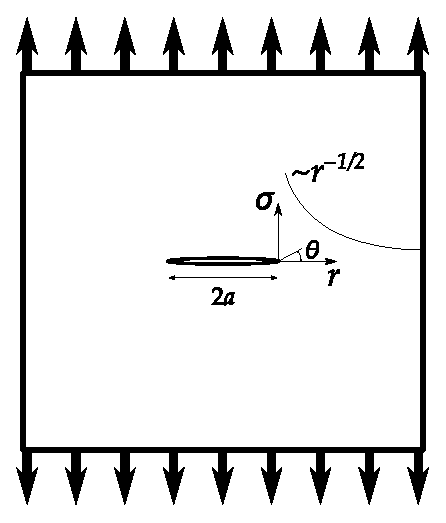
\includegraphics[width=0.5\hsize]{./img/cracktip_singularity.eps}
 \end{center}
 \caption{���Ͱ�ĥ�ٽŤ������̵��ʿ�Ĥ������¸�ߤ�����߷����δ��̤����Ȥ��Τ�����ü��˵�α����ð۾�}\label{fig:cracktip_singularity}
\end{figure}
\subsection{���ϳ��緸��}
������ɾ�����뤿����˲��ϳإѥ�᡼������ǺǤ�ͭ̾�Ǥ�����ϳ��緸���ˤĤ����������롣
�ܸ���ˤ����Ƥ���ϳ��緸�����Ѥ��롣
��\ref{fig:cracktip_singularity}�Τ褦�ʴ��̤�����ͭ����̵��ʿ�Ĥˤ����ơ�
ʿ�̤Ҥ��߾��֤α��ϥƥ󥽥�$\btns{\sigma}$�ȱ��ϳ��緸��$K_I$�Ȥδط���
\begin{equation}
 \sigma_{xx} = \frac{K_I}{\sqrt{2 \pi r}} \cos \frac{\theta}{2}
  \left(1 - \sin \frac{\theta}{2} \sin \frac{3 \theta}{2}\right),\label{eq:sif_sigma_xx}
\end{equation}
\begin{equation}
 \sigma_{yy} = \frac{K_I}{\sqrt{2 \pi r}} \cos \frac{\theta}{2}
  \left(1 + \sin \frac{\theta}{2} \sin \frac{3 \theta}{2}\right),\label{eq:sif_sigma_yy}
\end{equation}
\begin{equation}
 \sigma_{zz} = \nu (\sigma_{xx} + \sigma_{yy}),\label{eq:sif_sigma_zz}
\end{equation}
\begin{equation}
 \sigma_{xy} = \sigma_{yx} = \frac{K_I}{\sqrt{2 \pi r}}
  \sin \frac{\theta}{2} \cos \frac{\theta}{2} \cos \frac{3 \theta}{2},\label{eq:sigma_xy}
\end{equation}
\begin{equation}
 \sigma_{yz} = \sigma_{zy} = \sigma_{zx} = \sigma_{xz} = 0\label{eq:sif_sigma_yz}
\end{equation}
�Τ褦��ɽ���졢
�Ѱ̥٥��ȥ�$\bvec{u}$�Ȥδط���
\begin{equation}
 u_{x} = \frac{K_I}{G} \sqrt{\frac{r}{2 \pi}} \cos \frac{\theta}{2}
  \left(1 - 2 \nu + \sin^2 \frac{\theta}{2}\right),\label{eq:sif_u_x}
\end{equation}
\begin{equation}
 u_{y} = \frac{K_I}{G} \sqrt{\frac{r}{2 \pi}} \sin \frac{\theta}{2}
  \left(2 - 2 \nu - \cos^2 \frac{\theta}{2}\right),\label{eq:sif_u_y}
\end{equation}
\begin{equation}
 u_{z} = 0\label{eq:sif_u_z}
\end{equation}
�Τ褦��ɽ�����\cite{Shiratori1980, Yagawa1988}��
��������
$r$�Ϥ�����ü����ε�Υ��$\theta$�Ϥ����̤Ȥγ��١�
$\nu$�ϥݥ������桢$G$�Ϥ��������������Ǥ��롣
�ޤ���$K_I$��ź��$I$�ϡ�
�ٽ������������̤������ȿ�ľ�Ǥ���⡼�� I ����ñ���ٽž��Ǥ��뤳�Ȥ򼨤���
�ٽ������α���$\sigma_{yy}$��$r^{-\frac{1}{2}}$�����㤹����ǽ�ɽ����Ƥ��뤳�Ȥ����դ��롣

�˲��ϳؤǤϡ����ϳ��緸�����Ѥ��뤳�Ȥ���Ĥ�ɾ������ǽ�ˤʤ롣
����ܤ�ɾ���Ϥ������˲���ɾ���Ǥ��롣
�ޤ��������ʤ���������ʤ������ĥ��ϫ��ʤɤκ����¸��Ǻ�������Ǥ����˲���������$K_c$����롣
�˲��������ͤϥϥ�ɥ֥å�������Ƥ��ɤ���
�������ϳ��緸������Ӥ���
$K > K_c$�Ȥʤä��餼�����˲��򵯤�����
����ܤ�ɾ������ϫ�����ʤɤˤ����뤭���ο�Ÿ®�٤�ɾ���Ǥ��롣
������Ÿ®�٤ȱ��ϳ��緸���δط����ϸ�˽Ҥ٤� Paris §��ͭ̾�Ǥ��롣
\section{ͭ������ˡ�ˤ���˲��ϳز���}
\subsection{�׻��˲��ϳؤ�Ƴ��}
�˲��ϳؤ������Ǥϡ�
ñ��ʷ��������ñ��ʲٽž������ꤷ���������Ȥ��Ǥ��ʤ���
���Τ褦���طʤǡ�
ʣ�����������ʣ��ٽŤ�����򰷤�������˲��ϳؤΥ��ߥ�졼����󤬹Ԥ��Ƥ��롣
�˲��ϳؤΥ��ߥ�졼�����Ǥϡ�
����Ū�ʹ�¤���Ϥ�Ʊ����ͭ������ˡ���Ѥ���Τ�����Ū�Ǥ��롣
�˲��ϳإ��ߥ�졼�����ι����ϡ����λ��Ĥ��ʳ��򷫤��֤����ȤǹԤ��롣
\begin{enumerate}
 \item ������ޤ��å�����Ѥ���ͭ�����Dz��Ϥ�Ԥ���
 \item ���Ϸ�̤��Ѱ̤���Ϥ����˲��ϳإѥ�᡼�� (���ϳ��緸��) ����롣
 \item ������Ÿ®�٤�ɾ�������������Ÿ��������������å�����������롣
\end{enumerate}
���줾����ʳ��ˤĤ��ƽ��פ�����ʹߤξ�����������롣
\subsection{������ޤ��å���}
������ޤ��å�����Ѥ��ƹԤ�ͭ�����Dz��Ϥˤ�������פ����ϡ�
�����η�����ɽ�������å�����������뤳�ȤǤ��롣
���ˡ�
�˲��ϳز��ϤǤϤ�����ü��˵��$\mathrm{O} (r^{-\frac{1}{2}})$�α����ð۾��¿�༰������ͭ�����Ǥ�ɽ������ΤϺ���Ǥ��롣
����ˡ�
������ü��˵�����ǥ������ϡ�
���ϥ��ƥåפ�����Τ�����Ÿ�̤�ʬ��ɽ���������������ʤ���Фʤ�ʤ���
�����ǡ�
������ü��˵�Ǥ����˺٤�������ʬ���Ԥ���
������ü��˵����Υ���˽��ä�����ʬ����Ƥ�����褦�ʥ�å��󥰤�Ԥ�ɬ�פ����롣

�˲��ϳز��ϤǤΥ�å���ϡ�
��������̩���դ����Ƥ�������Ǥʤ���
������Ÿ��ɽ���Ǥ��ʤ���Фʤ�ʤ���
������Ÿ��ɽ��������ˡ������ढ�롣
����ܤ����Ǥ���Ǥ�������ˡ�Ǥ��롣
��������Ǥι����򥼥��ˤ��뤳�ȤǼ¸�������礬¿����
����ܤϡ���Ĥ���������Ĥ�ʬ����������ˡ�Ǥ��롣
���Ԥϥ����ǥ��󥰤��ưפǤ������������뤬��
������ü��ͭ�����Ǥ��դȤʤ�ͳѤ��ʤäƤ��ޤ����������롣
�ܸ���Ǥϡ�
������ü������˥�ǥ벽�Ǥ������ǥ�ǥ벽���٤ι⤤��Ԥ���Ѥ��롣
\subsection{ľ���Ѱ̳���ˡ�ˤ����ϳ��緸����ɾ��}
ͭ�����Dz��Ϥη�̤�����ϳ��緸���������ˡ��������ʬ�व��롣
����ܤ��Ѱ̤���Ϥ���ľ��Ū�˱��ϳ��緸���������ˡ�ǡ�ľ��ˡ�ȸƤФ�롣
����ܤϤҤ��ߥ��ͥ륮�����Ѳ��̤�����ϳ��緸���������ˡ�ǡ�
���ͥ륮��ˡ�ȸƤФ�롣
���Ԥˤ�ľ��Ū�Ǵ��ؤʤ��Ȥ����������ꡢ
��Ԥˤϰ��̤�ľ��ˡ�������٤Ǥ���Ȥ������������롣
���ͥ륮��ˡ�Ǥ�������������ʬ������ʬ��ϩ���Ѱդ���ɬ�פ����뤿�ᡢ
�ܸ���Ǥϴ��ؤ�ľ��ˡ���Ѥ��롣
ľ��ˡ�ˤϡ�
�� (\ref{eq:sif_sigma_xx}) ���鼰 (\ref{eq:sif_sigma_yz}) �ޤǤ�����ϳ��緸�������ľ�ܱ���ˡ�ȡ�
�� (\ref{eq:sif_u_x}) ���鼰 (\ref{eq:sif_u_z}) �ޤǤ������ľ���Ѱ�ˡ��ʬ����롣
���̤ˡ�
ͭ�����ǹ�¤���Ϥ��Ѱ�ˡ�ǹԤ����ᡢ
���Ϥ����Ѱ̤��������٤��ɤ����Ȥ��Τ��Ƥ��롣
�ޤ������Ϥ�������ʬ����ǵ�����Τ��Ф��ơ�
�Ѱ̤�������ǵ����뤿�᰷���䤹�����������롣
�ܸ���Ǥ�ľ���Ѱ�ˡ�ΰ��Ǥ���ľ���Ѱ̳���ˡ���Ѥ��롣

ľ���Ѱ̳���ˡ�ˤĤ����������롣
�ٽ������Ȥ����̤���������ľ�ʾ�硢
�� (\ref{eq:sif_u_y}) ��򤤤������Ѱ�$u_y$������ϳ��緸��$K_I$����롣
���ΤȤ���
������ü�������Ǥ��Ѱ�$u_y$�������ˤʤäƤ��ޤ���
�����ǡ�
�����̾��ʣ���������Ǽ� (\ref{eq:sif_u_y}) ������ϳ��緸�����ᡢ
����餫�鳰�ޤ��뤳�ȤǤ�����ü��������α��ϳ��緸������롣
�����̾�������Ǥ�$\theta = \pi$�Ǥ��뤳�Ȥ����դ��롣
���γ��ޤϿ�\ref{fig:direct_extrapolation_method}�Τ褦��ľ���ǹԤ���
�ʤ��ʤ顢
������ü��˵���ð����ϼ� (\ref{eq:sif_u_y}) �ǵۼ�����Ƥ��뤿��Ǥ��롣
������ü��˵�α��Ͼ��$\sigma \propto r^{-\frac{1}{2}}$�Ǥ��ä������Ѱ̾��$u \propto r^{\frac{1}{2}}$�Ǥ��뤳�Ȥ����դ��롣
�ޤ�����\ref{fig:direct_extrapolation_method}�Τ褦�ˡ�
������ü�������˰��ֶᤤ�����Ǥα��ϳ��緸���Ͼ������ɾ������뤳�Ȥ��Τ��Ƥ��롣
\begin{figure}[tbp]
 \begin{center}
  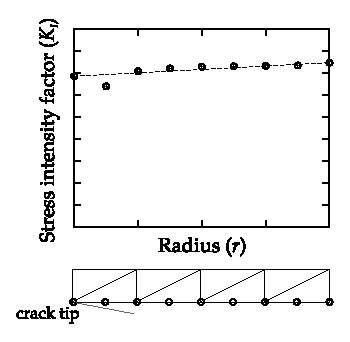
\includegraphics[width=0.6\hsize]{./img/direct_extrapolation_method.eps}
 \end{center}
 \caption{ľ���Ѱ̳���ˡ�ˤ����ϳ��緸����ɾ��}\label{fig:direct_extrapolation_method}
\end{figure}
\subsection{Paris §�ˤ�뤭����Ÿ®�٤�ɾ��}
���ϳ��緸�����餭����Ÿ®�٤������ˡ�Ȥ��ơ�
�褯�Ѥ����� Paris §�ˤĤ����������롣
Paris §����ϫ�˲���������ˡ�Ǥ��ꡢ
\begin{equation}
 \frac{\diff a}{\diff N} = C \Delta K^n\label{eq:paris_law}
\end{equation}
�Τ褦��ɽ����롣
�����ǡ�
$a$�Ϥ���Ĺ��$N$����ϫ�����������
$\diff a / \diff N$�Ϥ�����Ÿ®�١�
$\Delta K$�Ϻ�����ϳ��緸���ȺǾ����ϳ��緸���κ���
$C$��$n$�� Paris §�κ�������Ǥ��롣
�����忩���䥯�꡼�פ����ʤɤ���ϫ�˲��ʳ��Τ�����Ÿ���ݤǤϡ�
����$t$���Ф���$\diff a / \diff t$������Ÿ®�٤Ȥ��뤳�Ȥ�¿����
�ޤ���$\Delta K$��$\Delta K = K_{\max} - K_{\min} = K - 0 = K$�Ȥ��뤳�Ȥ�¿����

Paris §���Ѥ�����ϫ������Ÿ���Ϥ�Ԥ��Ȥ���
��Ĥ���ˡ�����롣
����ܤ���ˡ�ϡ�
���ϥ��ƥåפ�����Τ�����Ÿ��$\Delta a$����ꤷ�ơ�
\begin{equation}
 \Delta N \simeq \frac{1}{\diff a / \diff N} \Delta a
  = \frac{\Delta a}{C \Delta K^n}
\end{equation}
�Ȥ��Ƥ�����Ÿ�̤��Ф�����ϫ���������$\Delta N$���ᡢ
\begin{equation}
 N = \int \diff N \simeq \sum \Delta N
\end{equation}
�Τ褦����ϫ���������$N$�������ˡ�Ǥ��롣
����ܤ���ˡ�ϡ�
���ϥ��ƥåפ��������ϫ���������$\Delta N$����ꤷ�ơ�
\begin{equation}
 \Delta a \simeq \frac{\diff a}{\diff N} \Delta N
  = C \Delta K^n \Delta N
\end{equation}
�Τ褦�ˤ�����Ÿ��$\Delta a$�������ˡ�Ǥ��롣
���ΤȤ���
���ϥ��ƥå׿�����ϫ��������������������뤳�ȤϷ׻�����ǽ�����¤���Ԥ�ʤ��Τ�����Ū�Ǥ��롣
���̤ˡ���ϫ�����Ǥ���ϫ�����������¿���ʤ�ۤɿ�Ÿ®�٤��礭���ʤ뤿�ᡢ
������Ÿ�̤���ꤹ�������ϫ�������������ꤹ�����������٤ˤʤ롣
�������ʤ��顢
��å�����������������ܤ���ȡ�
���Ԥϥ�å����������Ԥ��䤹����å����ͽ���������뤳�Ȥ���ǽ�Ǥ��롣
������Ф��ơ�
��Ԥϥǥ����ˡ�����ʬ��ˡ�ʤɤ��Ѥ����ܳ�Ū�ʥ�å������������ϥ��ƥå���˹Ԥ�ɬ�פ����롣
�ޤ�����Ԥ���ˡ�Ǥϡ�
�Ʋ��ϥ��ƥåפǤ����ο�Ÿ��������뤳�ȤǶʤ��ä�������ɽ�����뤳�Ȥ��ǽ�Ǥ��롣
�ܸ���Ǥϡ�
ʬΥȿ��Ϣ����ˡ�μ�ˡ�򥪥ꥸ�ʥ�ƥ��Ȥ��뤿����ؤ����Ԥ��Ѥ����٥���ޡ�����Ԥ���
���������ܼ�ˡ�ϸ���Ū�ˤϸ�Ԥˤ�Ŭ�Ѳ�ǽ�Ǥ���ȹͤ����롣
\section{�絬�Ϥ��˲��ϳز��Ϥδ�¸��ˡ}
�˲��ϳز��Ϥ��絬�ϲ�����Ȥ��˵���������Ȥ�����Ф����¸��ˡ���������롣
�˲��ϳز��Ϥ��絬�ϲ�����Ȥ���
�ºݤ˼�ͳ�٤��礭���ʤ�ΤϤ�����ü��˵�ǤϤʤ�������ü���齽ʬ��Υ�줿�����ΰ�Ǥ��롣
�����ǡ�
������ü��˵�Ȥ����ɽ�Ū�ʾ������ΰ�Ǥ��˲��ϳز��Ϥ�Ԥ���
�������齽ʬ��Υ�줿����ʬ���ΰ�Ǥ������������Ϥ�Ԥ��褦����ά��ͭ���Ǥ��롣
�ܸ�����оݤǤ���ʬΥȿ��Ϣ����ˡ�⤳�ιͤ����˴�Ť��Ƥ��롣
���Τ褦�ʥ��ץ��������顢
�絬���˲��ϳز��ϸ����μ�ˡ�Ȥ��ơ�
�礭���׻��̤���Ƥ����̾��ͭ�����Dz��Ϥ�Ԥ���ˡ\cite{Okada2005, Okada2008}��¾�ˤ����Ĥ��μ�ˡ����Ƥ���Ƥ��롣
�����ߥ�ˡ����ӽŹ��å���ˡ\cite{Fish1992, Kikuchi2008}���������롣
����黰��ˡ�ˤĤ��ƽ���������롣

�̾��ͭ������ˡ�ˤ���絬���˲��ϳز��ϤǤϡ�
����ʤ����դ���å������������
����򾮵��ϲ��Ϥ�Ʊ�ͤˤ��Ʋ��Ϥ��롣
���ΤȤ���
��������Ÿ�����٤˵���ʤ����դ���å���κ�������Ԥ���
�ޤ���
�˲��ϳز��Ϥ�ޤ๽¤���ϤǤ�ϻ�������Ǥ�����Ū�Ǥ��뤬��
�絬�ϲ��Ϥξ��ϥǥ����ˡ�����ʬ��ˡ�ˤ����������Ǥ����ޤ�롣
Okada et al. �ϻ����ΰ켡���Ǥ���ӻ����������Ǹ����Υ��ͥ륮��ˡ�١����α��ϳ��緸����ɾ����ˡ����Ƥ��Ƥ���\cite{Okada2005, Okada2008}��

�����ߥ�ˡ���˲��ϳ�����ʤɤθ����ϳ�������̤ǹ����Ȥ��Ƥ����ˡ�Ǥ��롣
��\ref{fig:zooming}�Τ褦�ˡ�
�����ΰ����Τ��Ƥ���ǥ벽�����������Х��ǥ�$\varOmega^G$���Ф��������������Ϥ�Ԥ���
���θ塢
������ü��˵���ڤ�Ф������������ǥ�$\varOmega_L$���Ф����˲��ϳز��Ϥ�Ԥ���
���ΤȤ���
�������Х��ǥ�Υ�å�����Ƥ���
���������ǥ�Υ�å���Ϻ٤�������Τ�����Ū�Ǥ��롣
���������ǥ�ζ������ˤϥ������Х��ǥ�β��Ϸ�̤��Ѥ��뤬��
�������Х��ǥ�ȥ��������ǥ�Υ�å���ϰ��̤˶�������������԰��פǤ��뤿�ᡢ
�������μ����Ϥ����ˤ���֤�Ԥ�ɬ�פ����롣
�ޤ���
�����Ϥ��������϶����Ѱ̶���������ٽŶ��������������٤��ɤ��ʤ�ȸ����Ƥ��뤬��
�ٽŶ����������ǤϹ��Υ⡼�ɤ�«�Ǥ��ʤ��Τ���Ĥζ������򶭳�������˿���ʬ����ɬ�פ����롣
����ˡ������Ѱ̶��������Ѥ������ͭ�����Ǥη����ؿ������Ū�ưפ���֤��Ǥ��뤬��
�ٽŶ������ξ��������ٽŤ���ʤ���Фʤ餺���٤�ô�ݤ�����Ǥ��롣
�����ٽŤˤϡ�
��ʬ���夫�����������֤��줿����$\btns{\sigma}$��ñ��ˡ���٥��ȥ�$\bvec{n}$����
\begin{equation}
 \bvec{t} = \btns{\sigma} \bvec{n}
\end{equation}
�Τ褦�˵�᤿�ȥ饯�����$\bvec{t}$���Ѥ����롣
����ή���ϢΩ�켡��������ɽ������ȡ�
\begin{equation}
 \bvec{K}_G \bvec{u}_G = \bvec{f}_G\label{eq:zooming_global}
\end{equation}
��򤭡�
$\bvec{u}_G$���鲿�餫����ˡ��$\bvec{f}_L$����������
\begin{equation}
 \bvec{K}_L \bvec{u}_L = \bvec{f}_L
\end{equation}
��򤯤Ȥ���ή��ˤʤ롣
$\bvec{K}_G$�ϥ������Х�ι�������
$\bvec{K}_L$�ϥ�������ι�������
$\bvec{u}_G$�ϥ������Х�������Ѱ̥٥��ȥ롢
$\bvec{u}_L$�ϥ�������������Ѱ̥٥��ȥ롢
$\bvec{f}_G$�ϥ������Х�������ٽť٥��ȥ롢
$\bvec{f}_L$�ϥ�������������ٽť٥��ȥ�Ǥ��롣
����ή��Ϥ�����Ÿ���٤˹Ԥ��뤬��
�������Х��ǥ�ˤ������ǥ벽���ʤ���硢
�� (\ref{eq:zooming_global}) �ϲ��Ϥΰ��֤Ϥ���˰������򤫤�롣
�ʾ�Τ褦�ˡ�
���������ΰ�α������������Х��ΰ��ȿ�Ǥ���ʤ������ߥ�ˡ�Ǥϡ�
�������Х��ǥ�β��Ϸ�̤����١�
����ӡ�����������֤����٤ˤĤ��Ƶ��䤬�Ĥ롣
�ޤ���
���������ǥ���礭�����������������ǥ�ؤζ���������Ϳ�λ���������������뤿�ᡢ
���������٤��и��˺��������¦�̤����롣

�Ź��å���ˡ�ϥ����ߥ�ˡ�����٤����������ˡ�Ǥ��롣
�Ź��å���ˡ�Ǥϥ����ߥ�ˡ��Ʊ�ͤ˥������Х��ǥ뤪��ӥ��������ǥ���Ѱդ���
������Ʊ���˲��Ϥ��롣
���ΤȤ���
�����ߥ�ˡ��Ʊ�ͤ˥������Х��ǥ�ȥ��������ǥ�Υ�å���ϰ��̤����������פ��ʤ���
�ޤ��������ϥ��������ǥ�ˤΤߥ�ǥ벽����롣
�Ź��å���ˡ�ˤ�ä�������ϢΩ�켡��������
\begin{equation}
 \pmat{
  \begin{array}{cc}
   \bvec{K}_G & \bvec{K}_{GL} \\
   \bvec{K}_{GL}\trp & \bvec{K}_L \\
  \end{array}
  } \pvec{
  \begin{array}{c}
   \bvec{u}_G \\
   \bvec{u}_L \\
  \end{array}
  } = \pvec{
  \begin{array}{c}
   \bvec{f}_G \\
   \bvec{f}_L \\
  \end{array}
  }\label{eq:mesh_superposition}
\end{equation}
�Τ褦��2$\times$2�Υ֥��å������ޤ�����ˤʤ롣
$\bvec{K}_{GL}$�ϡ�
�������Х��ǥ�ȥ��������ǥ��饰��󥸥��̤����ˡ�ˤ�äƷ�ӤĤ����������Ǥ��롣
���μ�����ǡ�
$\bvec{K}_L$�Ϥ�������Ÿ�����٤˺���������뤳�Ȥ����դ��롣
�� (\ref{eq:mesh_superposition}) �ι���ϡ�
�饰��󥸥����αƶ��Ǿ������礭���ʤ뤳�Ȥ��Τ��Ƥ��롣
�ޤ���$\bvec{K}_{GL}$�αƶ��ǹ���ΥХ�������礭���ʤ롣
�ʤΤǡ�
�Ź��å���ˡ��ϢΩ�켡���������򤹤뤿��ˤ�ľ��ˡ��
�⤷���϶��Ϥ����������դ���ȿ��ˡ���Ѥ���ɬ�פ����롣
�Ĥޤꡢ
�Ź��å���ˡ�Dz��ϲ�ǽ������μ�ͳ�ٿ��������������С�����ǽ�����������롣

�ܸ���Ǥϡ�
�̾��ͭ�����Dz��ϡ������ߥ�ˡ���Ź��å���ˡ�λ���ˡ��դߤơ�
�̾��ͭ�����Dz��Ϥ���®�ǡ�
�����ߥ�ˡ��������٤ǡ�
�Ź��å���ˡ�Τ褦�������������С������������ʤ���ˡ�Ȥ��Ƹ�˽Ҥ٤�ʬΥȿ��Ϣ����ˡ����Ƥ��롣
\begin{figure}[tbp]
 \begin{center}
  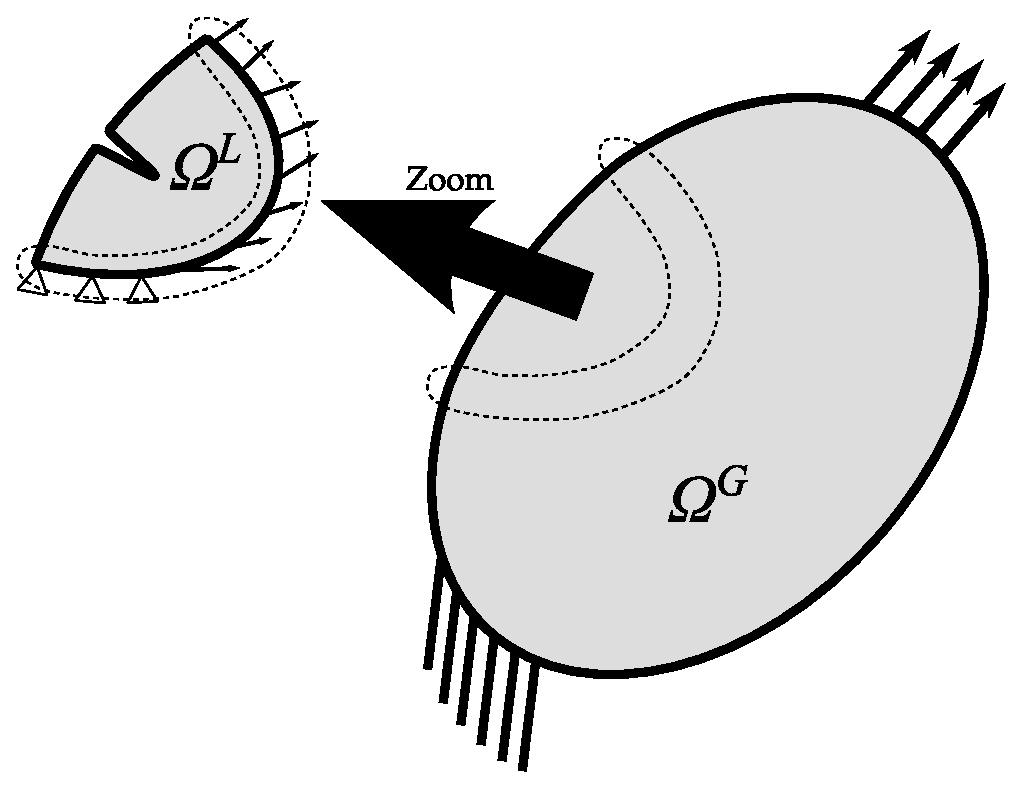
\includegraphics[width=0.7\hsize]{./img/zooming.eps}
 \end{center}
 \caption{�����ߥ�ˡ�Υ������Х��ǥ�ȥ��������ǥ�}\label{fig:zooming}
\end{figure}
\section{���}
�ܾϤǤϡ�
�˲��ϳؤ�����������ӷ׻��˲��ϳؤ���ˡ�ˤĤ�������������
�ޤ���
�׻��˲��ϳؤ��絬�ϲ��ϤΤ���δ�¸��ˡ�Ȥ��ơ�
�̾��ͭ������ˡ�������ߥ�ˡ���Ź��å���ˡ�λ���ˡ������������

%% -*- coding: euc-jp -*-
\chapter[�ޥ���ե����å���Ϣ�����Ϥ�ʬΥȿ����ˡ]{�ޥ���ե����å���Ϣ�����Ϥ� \\ ʬΥȿ����ˡ}
\section{���}
�ܾϤǤϡ�
�ޥ���ե����å���Ϣ�����Ϥ����Ϣ�����ϤγƼ�ˡ�ˤĤ�����������
���Ϥǿ��줿�絬���˲��ϳ���������δ�¸��ˡ��Ϣ�����ϼ�ˡ�Ȥ���ʬ�ह�롣
³���ơ�
�ܸ�����Ѥ���ʬΥȿ����ˡ��¾��Ϣ�����ϼ�ˡ�Ȥΰ㤤��Ҥ١�
ʬΥȿ����ˡ���Ѥ�����ȿ����������ˤĤ��ƽҤ٤롣
\section{Ϣ�����Ϥγ���}
Ϣ�����ϤȤϡ�
�ۤʤ������������ɽ�����ʣ�����������ߺ��Ѥ򰷤����ߥ�졼�����Τ��ȤǤ��롣
Ϣ�����Ϥϥޥ���ե����å������ϤȤ�ƤФ졢
�äˡ�
ή�Ρ���¤Ϣ������\cite{Zhang2001, Matthies2003, Tezduyar2007, Minami2010}��
���졦��¤Ϣ������\cite{Sugimoto2010}��
���ס���¤Ϣ�����Ϥλ��Ĥ�ͭ̾�Ǥ��롣
�ܸ���Ǥϡ�������Ϣ�����Ϥμ�ˡ��������ơ�
��¤����¤Ϣ�����Ϥ⤷���ϸ��Ρ�����Ϣ�����ϤȤ����褦�ʲ��Ϥ�Ԥ���
����ܤθ����ϳز��ϤȤ����絬�Ϥ��������ϡ�
����ܤθ����ϳز��ϤȤ��Ƥ�����ü��˵���˲��ϳز��Ϥ�Ԥ���
������Ϣ³����Ϣ�����ϼ�ˡ�ˤ�ä�ô�ݤ��롣
\section{Ϣ�����ϼ�ˡ��ʬ��}
Ϣ�����ϼ�ˡ�ϰ��̤ˡ�
ʬΥ��������Ϣ����ˡ��
ʬΥ��������������ˡ\cite{Sugimoto2010}��
ʬΥ��������ȿ����ˡ\cite{Matthies2003, Tezduyar2007, Minami2010}��
���η���ˡ\cite{Zhang2001}�λͼ����ʬ�व��롣
�ʹߡ�Ϣ��������Ĥθ��ݤ��ص����ǥ� 1����ǥ� 2 �ȸƤ֡�
��Ĥ���Ω����������������Υ���������ϢΩ�켡������
\begin{equation}
 \bvec{K}_1 \bvec{u}_1 = \bvec{f}_1,
\end{equation}
\begin{equation}
 \bvec{K}_2 \bvec{u}_2 = \bvec{f}_2
\end{equation}
�������롣
��������ߺ��Ѥ�
\begin{equation}
 \pmat{
  \begin{array}{cc}
   \bvec{K}_1 & \bvec{K}_{12} \\
   \bvec{K}_{12}\trp & \bvec{K}_2 \\
   \end{array}
   } \pvec{
   \begin{array}{c}
    \bvec{u}_1 \\
    \bvec{u}_2 \\
   \end{array}
   } = \pvec{
   \begin{array}{c}
    \bvec{f}_1 \\
    \bvec{f}_2 \\
   \end{array}
   }
\end{equation}
�Τ褦��ϢΩ�켡��������ɽ���롣
��������
$\bvec{K}_{12}$�ϥ�ǥ� 2 �����ǥ� 1 �ؤζ������μ����Ϥ���ɽ���������Ǥ��ꡢ
$\bvec{K}_{12}\trp$�ϥ�ǥ� 1 �����ǥ� 2 �ؤζ������μ����Ϥ���ɽ���������Ǥ��롣
���μ����Ѥ��Ƥ��λͼ���μ�ˡ�ˤĤ����������롣
�ʹߡ�
Ϣ�����븽�ݤο��ϴ���Ū����ĤȲ��ꤷ��
ư���ϡ���ʬ���ϡ�������Ÿ���Ϥʤɤβ��餫�λ��ּ�����Ĥ褦�ʲ��Ϥ��оݤȤ��롣

ʬΥ����ˡ�Ǥ������������������ʬΥ�������줾�����Ω�˲򤯡�
������Ϣ����ˡ�Ǥϡ�
��ǥ� 1 ��򤤤��塢
���β��Ϸ�̤���Ŭ����ʪ���̤��������
����ʪ���̤򶭳����Ȥ��ƥ�ǥ� 2 ��򤯡�
���ΤȤ���
��ǥ� 2 �β��Ϸ�̤ϥ�ǥ� 1 �β��Ϸ�̤ˤ�ȿ�Ǥ���ʤ���
ʬΥ��������Ϣ����ˡ�Υ��르�ꥺ���
\begin{algorithmic}
 \STATE $t \leftarrow 0$
 \WHILE{$t < t_{\max}$}
 \STATE $\bvec{u}_1^{(t)} \leftarrow \bvec{K}_1^{(t)^{-1}} \bvec{f}_1^{(t)}$
 \STATE $\bvec{u}_2^{(t)} \leftarrow \bvec{K}_2^{(t)^{-1}}
 \left(\bvec{f}_2^{(t)} - \bvec{K}_{12}^{(t)\trp} \bvec{u}_1^{(t)}\right)$
 \STATE $t \leftarrow t + 1$
 \ENDWHILE
\end{algorithmic}
�Τ褦�ˤʤ롣
�����ǡ�$t$�ϻ��֥��ƥåפǤ��ꡢ$t_{\max}$�Ͻ�λ���֤Ǥ��롣
���Υ��르�ꥺ����ϼ��ޤˤ���ȿ�\ref{fig:coupling_oneway}�Τ褦�ˤʤ롣

ʬΥ����������ˡ�ϡ�
�������Ȥϰ㤤��ǥ� 2 �β��Ϸ�̤���ǥ� 1 �β��Ϸ�̤�ȿ�Ǥ�����ˡ�Ǥ��롣
������ˡ��ȿ����ˡ��ʬ�व��롣
������ˡ�ϰ�����λ��֥��ƥåפ�$\bvec{u}_2^{(t-1)}$�򻲾Ȥ���
\begin{algorithmic}
 \STATE $t \leftarrow 0$
 \WHILE{$t < t_{\max}$}
 \STATE $\bvec{u}_1^{(t)} \leftarrow \bvec{K}_1^{(t)^{-1}}
 \left(\bvec{f}_1^{(t)} - \bvec{K}_{12}^{(t)} \bvec{u}_2^{(t-1)}\right)$
 \STATE $\bvec{u}_2^{(t)} \leftarrow \bvec{K}_2^{(t)^{-1}}
 \left(\bvec{f}_2^{(t)} - \bvec{K}_{12}^{(t)\trp} \bvec{u}_1^{(t)}\right)$
 \STATE $t \leftarrow t + 1$
 \ENDWHILE
\end{algorithmic}
�Τ褦��ɽ���Ǥ��롣
���Υ��르�ꥺ����ϼ��ޤˤ���ȿ�\ref{fig:coupling_staggered}�Τ褦�ˤʤ롣
���Ȥ��С�
��ǥ� 1 �����ǥ� 2 �˥Υ��ޥ󶭳������Ϥ����Ȥ����顢
��ǥ� 2 �����ǥ� 1 ���᤹�������ϥǥ��ꥯ�춭�����Ǥʤ���Фʤ�ʤ���
������ˡ���Ф��ơ�
���֥��ƥå���˥�ǥ� 1 �ȥ�ǥ� 2 ����ߺ��Ѥ�̩�˲��Ϥ���Τ�ȿ����ˡ�Ǥ��롣
�ܸ���ǤϤ�����Ѥ��롣
ʬΥ��������ȿ����ˡ�Υ��르�ꥺ���
\begin{algorithmic}
 \STATE $t \leftarrow 0$
 \WHILE{$t < t_{\max}$}
 \STATE $k \leftarrow 0$
 \WHILE{not converged}
 \STATE $\bvec{u}_1^{(t, k)} \leftarrow \bvec{K}_1^{(t, k)^{-1}}
 \left(\bvec{f}_1^{(t, k)} - \bvec{K}_{12}^{(t, k)} \bvec{u}_2^{(t, k-1)}\right)$
 \STATE $\bvec{u}_2^{(t, k)} \leftarrow \bvec{K}_2^{(t, k)^{-1}}
 \left(\bvec{f}_2^{(t, k)} - \bvec{K}_{12}^{(t, k)\trp} \bvec{u}_1^{(t, k)}\right)$
 \STATE $k \leftarrow k + 1$
 \ENDWHILE
 \STATE $t \leftarrow t + 1$
 \ENDWHILE
\end{algorithmic}
�Τ褦�ˤʤ롣
�����ǡ�$k$��ȿ�����ƥåפǤ��롣
���Υ��르�ꥺ����ϼ��ޤˤ���ȿ�\ref{fig:coupling_iterative}�Τ褦�ˤʤ롣
���ΤȤ�����ǥ� 1 ����������Ǥ����$\bvec{K}_1^{(t, k)} = \bvec{K}_1^{(t)}$�Ȥʤꡢ
��ǥ� 2 ����������Ǥ����$\bvec{K}_2^{(t, k)} = \bvec{K}_2^{(t)}$�Ȥʤ롣
�ޤ���ʬΥ��������ȿ����ˡ��ʬΥȿ����ˡ�Ȥ�ƤФ�롣

���η���ˡ��
\begin{algorithmic}
 \STATE $t \leftarrow 0$
 \WHILE{$t < t_{\max}$}
 \STATE $\pvec{
 \begin{array}{c}
  \bvec{u}_1^{(t)} \\
  \bvec{u}_2^{(t)} \\
 \end{array}
 } \leftarrow \pmat{
 \begin{array}{cc}
  \bvec{K}_1^{(t)} & \bvec{K}_{12}^{(t)} \\
  \bvec{K}_{12}^{(t)\trp} & \bvec{K}_2^{(t)} \\
 \end{array}
 }^{-1} \pvec{
 \begin{array}{c}
  \bvec{f}_1^{(t)} \\
  \bvec{f}_2^{(t)} \\
 \end{array}
 }$
 \STATE $t \leftarrow t + 1$
 \ENDWHILE
\end{algorithmic}
�Τ褦�ˡ�
$\bvec{K}_{12}$��Ƴ��������ĤΥ�ǥ��Ʊ���˲򤯼�ˡ�Ǥ��롣
���Υ��르�ꥺ����ϼ��ޤˤ���ȿ�\ref{fig:coupling_monolithic}�Τ褦�ˤʤ롣
$\bvec{K}_{12}$�ϥ饰��󥸥��̤����ˡ�ˤ�äƵ��롣
\begin{figure}[tbp]
 \begin{center}
  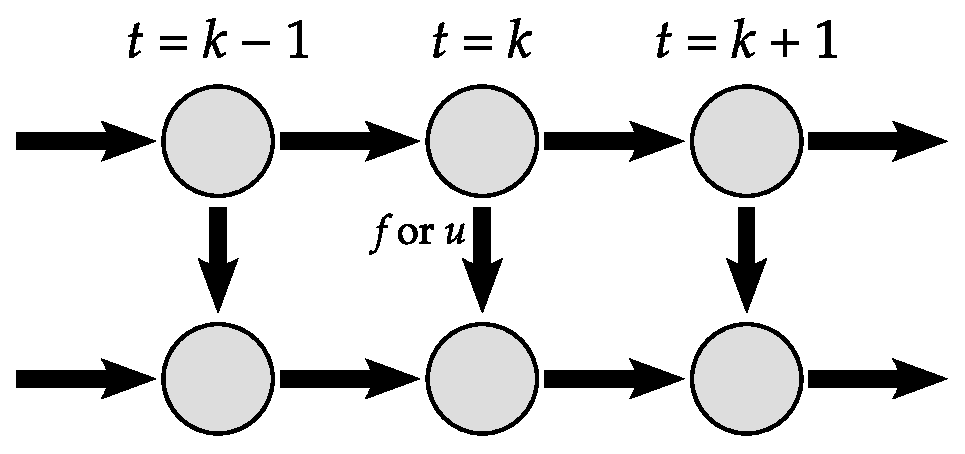
\includegraphics[width=0.7\hsize]{./img/coupling/oneway.eps}
 \end{center}
 \caption{ʬΥ��������Ϣ����ˡ���ϼ���}\label{fig:coupling_oneway}
\end{figure}
\begin{figure}[tbp]
 \begin{center}
  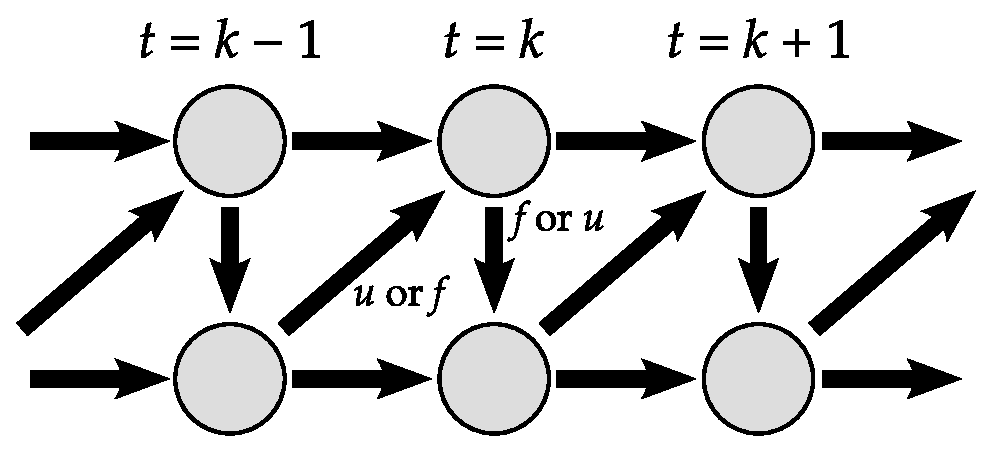
\includegraphics[width=0.7\hsize]{./img/coupling/staggered.eps}
 \end{center}
 \caption{ʬΥ��������������ˡ���ϼ���}\label{fig:coupling_staggered}
\end{figure}
\begin{figure}[tbp]
 \begin{center}
  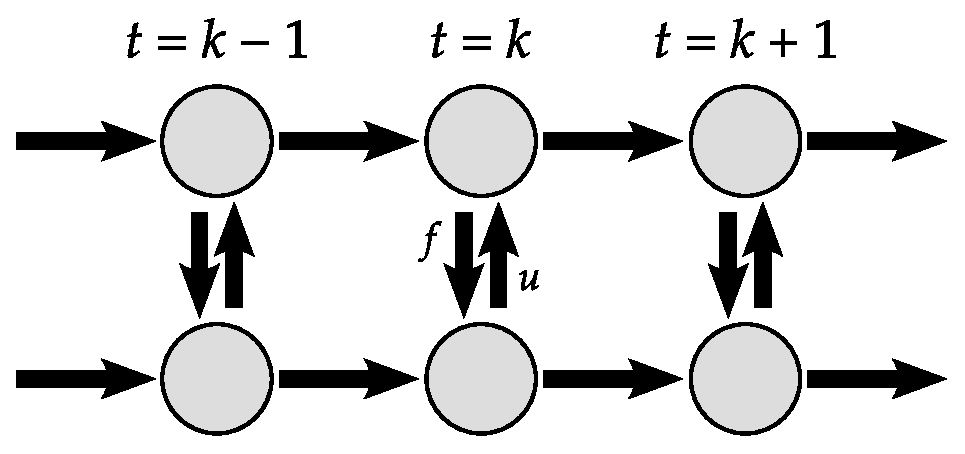
\includegraphics[width=0.7\hsize]{./img/coupling/iterative.eps}
 \end{center}
 \caption{ʬΥ��������ȿ����ˡ���ϼ���}\label{fig:coupling_iterative}
\end{figure}
\begin{figure}[tbp]
 \begin{center}
  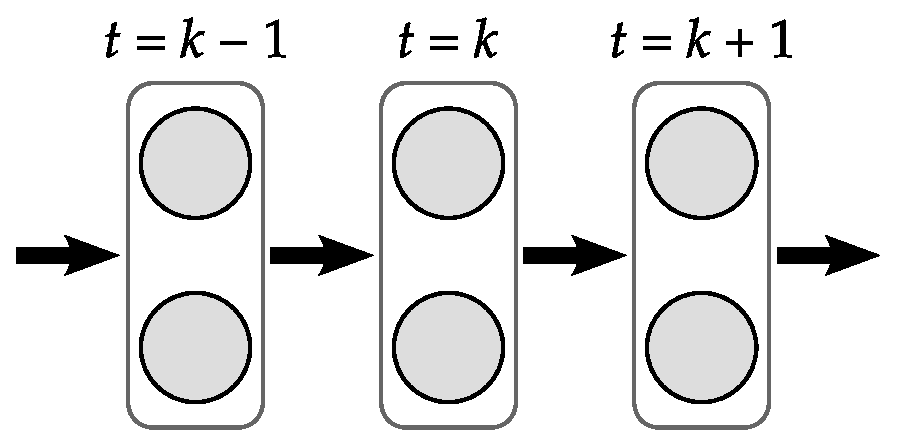
\includegraphics[width=0.7\hsize]{./img/coupling/monolithic.eps}
 \end{center}
 \caption{���η���ˡ���ϼ���}\label{fig:coupling_monolithic}
\end{figure}
\section{�絬���˲��ϳز��ϼ�ˡ��Ϣ�����ϼ�ˡ�Ȥ��Ƥ�ʬ��}
���ϤǽҤ٤��絬���˲��ϳز��Ϥδ�¸��ˡ��Ϣ�����Ϥλ�����ʬ�ह���ɽ\ref{tab:coupling_methods}�Τ褦�ˤʤ롣
Overlapping ����� Non-overlapping ���ܸ����Ƴ�����������Ǥ��ꡢ
��\ref{fig:overlapping_non_overlapping}�Τ褦�ˡ�
���������ǥ�򥰥����Х��ǥ�˽Ťͤ��碌�뤫�ݤ���ɽ����
¿����ή�Ρ���¤Ϣ�����Ϥ����ס���¤Ϣ�����Ϥϡ�
�����ΰ褬�Ťʤ���ʤ������ܼ�Ū�� Non-overlapping �Ǥ���\cite{Matthies2003, Tezduyar2007, Minami2010}��
������
���졦��¤Ϣ�����Ϥ��ż��Ϥ�ʪ���ϤȤ��ƺ��Ѥ��뤿���ܼ�Ū�� Overlapping �Ǥ���\cite{Sugimoto2010}��
�������Ф��ơ�
�ܸ�����оݤǤ��빽¤����¤Ϣ�����ϤǤ� Overlapping��Non-overlapping �Τɤ��餫�����򤹤뤳�Ȥ���ǽ�Ǥ��롣
���ơ����ϤǽҤ٤��絬���˲��ϳز��ϼ�ˡ���˸��Ƥ�����
�����ߥ�ˡ�� Overlapping ����ʬΥ��������Ϣ���Ǥ��롣
�ʤ���
Non-overlapping ����ʬΥ��������Ϣ���ϡ�
��\ref{fig:overlapping_non_overlapping}�α��ޤ褦�˥������Х��ǥ�˵�����ڤ�礭��¸�ߤ��뤳�ȤˤʤäƤ��ޤ����ḽ��Ū�Ǥʤ��ȹͤ����롣
�Ź��å���ˡ�� Overlapping ���ΰ��η���ˡ�Ǥ��롣
���ڤ�ϽŹ��å���ˡ����������������Ѥ���ȿ��Ū�ʲ��Ϥ�ԤäƤ���\cite{Suzuki1999, Suzuki2002}��
�̾��ͭ������ˡ�ˤ���˲��ϳز��Ϥϡ�
ʣ�������ǹ�����������ι��������­����碌��Ȥ����������� Non-overlapping ���ΰ��η���ˡ�Ȳ�᤹�뤳�Ȥ��Ǥ��롣

�����ǡ�
������Ÿ���ϸ����ǤϤʤ����絬�ϸ��β��Ϥμ�ˡ��ͤľҲ𤹤롣
����ܤ��ΰ�ʬ��ˡ\cite{Yagawa1991, Yagawa1993, Yagawa1993_2}�Ǥ��롣
�ΰ�ʬ��ˡ�ϥ����ѡ�����ԥ塼���� PC ���饹���ξ�Ǥ��絬�����������β��ϤǼ��Ӥ�����\cite{ADVENTURE, Yoshimura2002, Ogino2005}��
�ΰ�ʬ��ˡ�Ǥϡ�
��\ref{fig:ddm}�Τ褦��ʬ�䤵�줿�ΰ������˲��Ϥ���
�����ȿ�����뤳�Ȥ����Τβ����롣
�����������ΰ�ʬ��ˡ�� Non-overlapping ����ʬΥ��������ȿ����ˡ�ȸ����롣
�ܸ���Ǥϡ�
������ü��˵�Τ褦�˶ɽ�Ū��ʣ���������ܤ��뤿���ΰ�ʬ��ˡ�Υ��ץ�������ͭ���ǤϤʤ���
����ܤ϶Ѽ���ˡ\cite{Terada2001}�Ǥ��롣
�Ѽ���ˡ�ϼ���Ū�ʹ�¤�����������оݤȤ��� Overlapping ���ΰ��η���ˡ�Ǥ��롣
�Ѽ���ˡ���ΰ�ʬ��ˡ��Ʊ�ͤ˶ɽ�Ū��ʣ�������Ф��Ƥ�ͭ���ǤϤʤ���
�����ܤ� Nishikawa et al. ����Ƥ���ȿ�����֥��ȥ饯����ˡ\cite{Nishikawa2007}�Ǥ��롣
ȿ�����֥��ȥ饯����ˡ���絬�����������������Ƥ��줿��ˡ�Ǥ��ꡢ
ȿ��Ū�ʽŹ��å���ˡ�Ȼ������르�ꥺ��� Overlapping ����ʬΥ��������ȿ����ˡ�Ǥ��롣
�ͤ��ܤ� Yamada et al. ����Ƥ���
���ߤ⸦���ԤʤäƤ����ΰ�ʬ�䷿�Ź��å���ˡ�Ǥ���\cite{Yamada2011}��
����� Non-overlapping ���ΰ��η���ˡ�Ǥ��ꡢ
�ΰ�ֶ��������������פ��ʤ����˥��ͥ륮������¸����褦�������ˡ������Ū�˸��椵��Ƥ��롣

�ʾ�λͤĤμ�ˡ��¾�ˡ�
�������Х��ΰ�β��Ϥ�ͭ������ˡ�ǹԤ������������ΰ�β��Ϥ�ͭ������ˡ�ʳ�����ˡ�ǹԤ��褦���˲��ϳز��ϼ�ˡ����ľҲ𤹤롣
����ܤ�ͭ�����Ǹ��巫���֤�ˡ\cite{Nishioka1983}�Ǥ��롣
ͭ�����Ǹ��巫���֤�ˡ�Υ��������ΰ���˲��ϳؤ�������ǵ���褦�� Overlapping ����ʬΥ��������ȿ����ˡ�Ǥ��롣
���ϳ��緸���η׻�����������Ѥ���Τǡ�
�����������ξ���ɽ�̤��������פ����ʤɤ����Ūñ��ʷ����Τ������������ʤ��Ȥ������������롣
����ܤϳ�ĥͭ������ˡ\cite{Nagashima2003}�Ǥ��롣
��ĥͭ������ˡ�Ǥϡ�
ͭ�����Ǥ����޴ؿ��ˤ���������ɽ������ؿ���Ťͤ��碌�롣
���νŤ͹�碌��ؿ�����������ΰ��ª����ȡ�
��ĥͭ������ˡ�� Overlapping ���ΰ��η���ˡ�Ǥ��롣
��ĥͭ������ˡ��ʣ���ʷ����Τ����򰷤����Ȥ��Ǥ��뤬��
�Ź��å���ˡ��Ʊ�ͤ˹�������ξ������礭���ʤ뤿�ᡢ
�絬�ϲ����ˤ������������С������������롣
�ܸ���Ǥϡ�
ʣ�������λ����������򰷤����Ȥ���������Ƥ���Τǥ��������ΰ�β��Ϥˤ�ͭ������ˡ���Ѥ��롣

�ʾ�Τ褦�ʴ�¸�γƼ�ˡ���Ф��ơ�
�ܸ���Ǥ� Non-overlapping ����ʬΥ��������ȿ����ˡ���Ѥ��롣
������Ѥ�����åȤˤĤ��Ƥϼ���ǽҤ٤롣
\begin{table}[tbp]
 \caption{�絬���˲��ϳز��ϼ�ˡ��Ϣ�����ϼ�ˡ�Ȥ��Ƹ����Ȥ���ʬ��}\label{tab:coupling_methods}
 \begin{center}
  \small
  \begin{tabular}{l|cc}
   \hline
   & Overlapping & Non-overlapping \\
   \hline
   \hline
   ʬΥ��������     & �����ߥ�ˡ   & N/A \\
   \hline
   ʬΥ������������ & N/A            & N/A \\
   \hline
   ʬΥ��������ȿ�� & ���ڤ�νŹ��å���ˡ\cite{Suzuki1999, Suzuki2002} & �ΰ�ʬ��ˡ \\
   {}               & ȿ�����֥��ȥ饯����ˡ\cite{Nishikawa2007} & �ܸ��� \\
   {}               & ͭ�����Ǹ��巫���֤�ˡ & \\
   \hline
   ���η�           & �Ź��å���ˡ & (�̾��ͭ������ˡ) \\
   {}               & �Ѽ���ˡ       & �ΰ�ʬ�䷿�Ź��å���ˡ\cite{Yamada2011} \\
   {}               & ��ĥͭ������ˡ & \\
   \hline
  \end{tabular}
 \end{center}
\end{table}
\begin{figure}[tbp]
 \begin{center}
  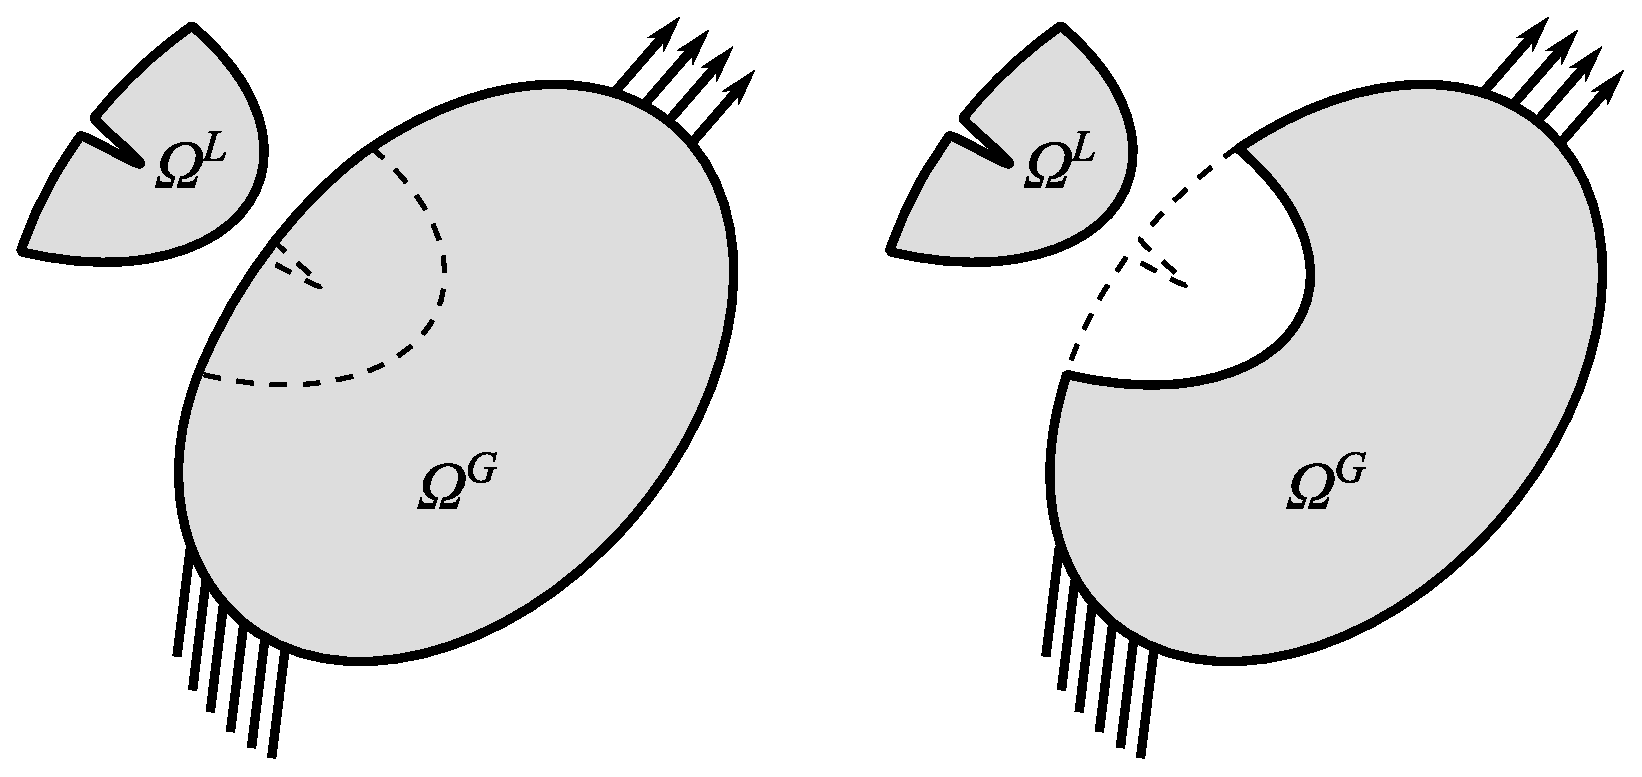
\includegraphics[width=\hsize]{./img/overlapping_non_overlapping.eps}
 \end{center}
 \caption{Overlapping ����ʬ�� (��) �� Non-overlapping ����ʬ�� (��)}\label{fig:overlapping_non_overlapping}
\end{figure}
\begin{figure}[tbp]
 \begin{center}
  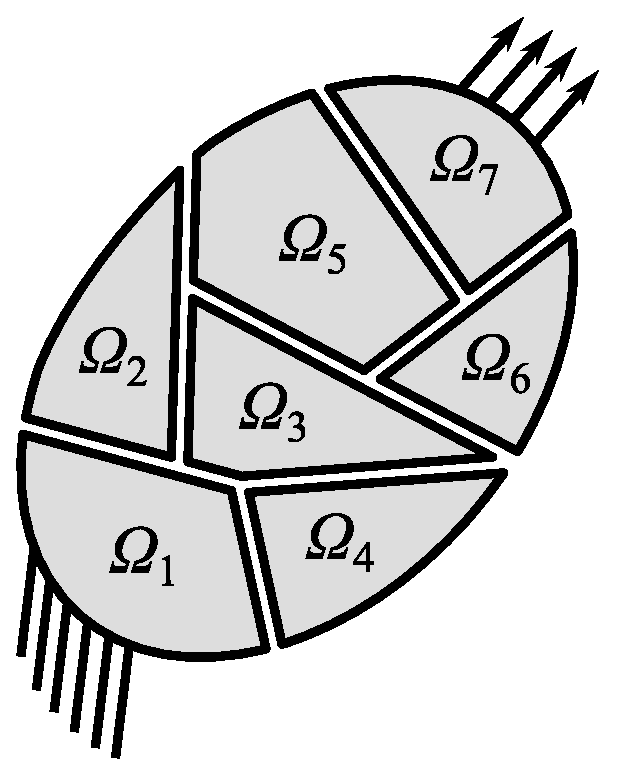
\includegraphics[width=0.4\hsize]{./img/ddm.eps}
 \end{center}
 \caption{�ΰ�ʬ��ˡ���ΰ�ʬ��}\label{fig:ddm}
\end{figure}
\section{ʬΥȿ����ˡ����ħ}
ʬΥȿ����ˡ�� Matthies and Steindorf �ˤ��ή�Ρ���¤Ϣ�����ϸ�������Ƥ��줿��ˡ�Ǥ���\cite{Matthies2003}��
ʬΥȿ����ˡ�Ǥϡ�
ʣ���θ��ݤΤ��줾�����Ω�˲򤭡�
������ȿ�����뤳�ȤǤ�����֥��ƥåפǤκǽ�Ū�ʲ�����롣
ȿ���׻��Ǹ����򾮤������Ƥ��뤿�ᡢ
��������ˡ�����������������ˡ��������٤ʲ�����뤳�Ȥ��Ǥ��롣
�ޤ���
��«Ƚ������ͤ�ʬ�˾���������а��η���ˡ��Ʊ���٤˹⤤���٤β�����뤳�Ȥ��Ǥ��롣
�������ʤ��顢
ʬΥȿ����ˡ�Ǥ�ȿ�������ʬ����¿���β��Ϥ�Ԥ�ʤ���Фʤ�ʤ����ᡢ
�׻�®�٤�������ϰ��η���ˡ���������ޤ�뷹���ˤ��롣
������
ʬΥȿ����ˡ�ǤϳƸ��ݤ���Ω�˲��Ϥ��뤿�ᡢ
��¸���θ�����Ω�Ƥ䤹���Ȥ������������롣
���Ȥ��С�ή�Ρ���¤Ϣ�����Ϥˤ����ơ�
��ή��ǥ���Ѥ���ͭ�º�ʬˡ���󰵽���Ǵ��ή�β��ϥ���С��ȹ���ǽ���Ǥ��Ѥ���ͭ������ˡ�����ѷ����ϥ���С���Ϣ��������褦�ʲ��Ϥ��ߤ�Ȥ���
ʬΥȿ����ˡ���Ѥ��Ƽ��ӤΤ��뤽�줾��Υ����ɤ��Ȥ߹�碌����ˡ�����ޤ�롣

�ܸ����ʬΥȿ����ˡ���Ѥ��Ƥ��뤿��ʾ�Τ褦�����������롣
�ܼ�ˡ���Ѥ��뤳�ȤǾ���Ū�ˤϡ�
�����ѡ�����ԥ塼�����ư����絬��������ϥ���С��Ⱥ����¸�����Ƴ���줿ʣ���ʹ��������Ȥ߹��ޤ줿�������������ϥ���С����Ȥ߹�碌�뤳�Ȥ���ǽ�Ȥʤ뤳�Ȥ��ͤ����롣
����˲ä��ơ�
�ܸ���ǤϤ�����Ÿ���ϤȤ���ʸ̮���顢
�����������С���������褫���ư��η���ˡ�����®��ʬΥȿ����ˡ�μ�����ԤäƤ��롣
����ˤĤ��Ƥϼ��ϤǾܺ٤˽Ҥ٤롣
\section{ʬΥȿ����ˡ��ȿ����������}
Ϣ������ʬ���ʬΥȿ����ˡ��ȿ����������Ȥ��ơ�
�֥��å� Jacobi ˡ��
�֥��å� Gauss--Seidel ˡ\cite{Tezduyar2007}��
Broyden ˡ\cite{Kelley2003}��
Newton--Krylov ˡ\cite{Kelley2003}���褯�Ѥ�����\cite{Minami2010}��
�֥��å� Jacobi ˡ�ϰ켡��«������ȿ��ˡ�ΰ��Ǥ��ꡢ
��ĤΥ�ǥ��Ʊ���˲򤱤�Ȥ�����ħ�����롣
2$\times$2�Υ֥��å������ޤ�ϢΩ������
\begin{equation}
 \pmat{
  \begin{array}{cc}
   \bvec{K}_1 & \bvec{K}_{12} \\
   \bvec{K}_{12}\trp & \bvec{K}_2 \\
  \end{array}
  } \pvec{
  \begin{array}{c}
   \bvec{u}_1 \\
   \bvec{u}_2 \\
  \end{array}
  } = \pvec{
  \begin{array}{c}
   \bvec{f}_1 \\
   \bvec{f}_2 \\
  \end{array}
  }
\end{equation}
�������������С��� Jacobi ˡ�Τ褦��
\begin{algorithmic}
 \STATE $k \leftarrow 0$
 \WHILE{not converged}
 \STATE $\bvec{u}_1^{(k)} \leftarrow \bvec{K}_{1}^{-1} (\bvec{f}_1 - \bvec{K}_{12} \bvec{u}_2^{(k-1)})$
 \STATE $\bvec{u}_2^{(k)} \leftarrow \bvec{K}_{2}^{-1} (\bvec{f}_2 - \bvec{K}_{12}\trp \bvec{u}_1^{(k-1)})$
 \STATE $k \leftarrow k + 1$
 \ENDWHILE
\end{algorithmic}
�ȹԤ�����֥��å� Jacobi ˡ�ȸƤФ�롣
������������� 3 ���ܤ� 4 ���ܤ�Ʊ���˼¹ԤǤ��롣
�ޤ���ʬΥȿ����ˡ�ˤ��Ϣ�����ϤǤ�$\bvec{K}_{12}$���ۤ��������뤳�ȤϾ��ʤ���
$\bvec{K}_{12}$�϶�����Υǥ��ꥯ�춭����� (�⤷���ϥΥ��ޥ󶭳����) �μ����Ϥ���
$\bvec{K}_{12}\trp$�ϥΥ��ޥ󶭳���� (�⤷���ϥǥ��ꥯ�춭�����) �μ����Ϥ���ɽ����
�֥��å� Gauss--Seidel ˡ��֥��å� Jacobi ˡ��Ʊ�ͤ�����ȿ��ˡ�ΰ��Ǥ��롣
�֥��å� Jacobi ˡ��Ʊ�ͤ�ϢΩ�������������������С��� Gauss--Seidel ˡ�Τ褦��
\begin{algorithmic}
 \STATE $k \leftarrow 0$
 \WHILE{not converged}
 \STATE $\bvec{u}_1^{(k)} \leftarrow \bvec{K}_{1}^{-1} (\bvec{f}_1 - \bvec{K}_{12} \bvec{u}_2^{(k-1)})$
 \STATE $\bvec{u}_2^{(k)} \leftarrow \bvec{K}_{2}^{-1} (\bvec{f}_2 - \bvec{K}_{12}\trp \bvec{u}_1^{(k)})$
 \STATE $k \leftarrow k + 1$
 \ENDWHILE
\end{algorithmic}
�ȹԤ�����֥��å� Gauss--Seidel ˡ�ȸƤФ�롣
������������� 3 ���ܤ� 4 ���ܤ˰�¸�ط������ꡢ
������Ʊ���˼¹Ԥ��뤳�ȤϤǤ��ʤ���
�������ꡢƱ���켡��«�μ�ˡ�Ǥ�֥��å� Gauss--Seidel ˡ�ϥ֥��å� Jacobi ˡ������̤�ȿ��������������ʤ�ȸ����Ƥ��롣
Yamada and Yoshimura �ϥ֥��å� Gauss--Seidel ˡ����ɤ���ľ��õ��ˡ��ή�Ρ���¤Ϣ�����ϸ�������Ƥ��Ƥ���\cite{Yamada2008}��
Broyden ˡ��Ķ�켡��«�ν� Newton ˡ�˴�Ť�Ϣ�����ϼ�ˡ�Ǥ��롣
Newton--Krylov ˡ�� Krylov ��ʬ���֤��󼡼�«�� Newton ˡ��Ԥ��褦��Ϣ�����ϼ�ˡ�Ǥ��롣
Newton ˡ�ʤΤǥ䥳�ӹ���ɬ�פǤ��뤬��
�䥳�ӹ�����ۤ��������ʤ� Newton--Krylov ˡ�� Jacobian-free Newton--Krylov ˡ�ȸƤФ�롣

�ޤ���
��¤����¤Ϣ�����ϼ�ˡ�Ȳ��Ǥ����¸��ˡ��ȿ����������ˤĤ��Ƥ�Ҳ𤹤롣
�äˡ��֥��å� Gauss--Seidel ˡ�ʳ��Τ�Τ�Ҳ𤹤롣
���ڤ��ȿ��Ū�ʽŹ��å���ˡ\cite{Suzuki1999, Suzuki2002}�ϥ֥��å� Gauss--Seidel ˡ���������դ��������ˡ���Ѥ��Ƥ��롣
�������դ��������ˡ�Υ��르�ꥺ��ϡ�
����������$\bvec{M}$���٥��ȥ�$\bvec{r}$��$\bvec{z}$��$\bvec{p}$��$\bvec{q}$��������ѿ�$\alpha$��$\beta$��$k$���Ѥ���
\begin{algorithmic}
 \STATE $k \leftarrow 0$
 \STATE $\bvec{r}^{(0)} \leftarrow \bvec{f} - \bvec{K} \bvec{u}^{(0)}$
 \STATE $\bvec{z}^{(0)} \leftarrow \bvec{M}^{-1} \bvec{r}^{(0)}$
 \STATE $\bvec{p}^{(0)} \leftarrow \bvec{z}^{(0)}$
 \WHILE{$||\bvec{r}^{(k)}|| / ||\bvec{b}^{(k)}||$ is not small enough}
 \STATE $\bvec{q}^{(k)} \leftarrow \bvec{K} \bvec{p}^{(k)}$
 \STATE $\alpha^{(k)} \leftarrow (\bvec{r}^{(k)}, \bvec{z}^{(k)}) / (\bvec{p}^{(k)}, \bvec{q}^{(k)})$
 \STATE $\bvec{u}^{(k+1)} \leftarrow \bvec{u}^{(k)} + \alpha^{(k)} \bvec{p}^{(k)}$
 \STATE $\bvec{r}^{(k+1)} \leftarrow \bvec{r}^{(k)} - \alpha^{(k)} \bvec{q}^{(k)}$
 \STATE $\bvec{z}^{(k+1)} \leftarrow \bvec{M}^{-1} \bvec{r}^{(k+1)}$
 \STATE $\beta^{(k)} \leftarrow (\bvec{r}^{(k+1)}, \bvec{z}^{(k+1)}) / (\bvec{r}^{(k)}, \bvec{z}^{(k)})$
 \STATE $\bvec{p}^{(k+1)} \leftarrow \bvec{z}^{(k+1)} + \beta^{(k)} \bvec{p}^{(k)}$
 \STATE $k \leftarrow k + 1$
 \ENDWHILE
\end{algorithmic}
�Τ褦��ɽ���뤬��
���󡦥٥��ȥ���$\bvec{q}^{(k+1)} \leftarrow \bvec{K} \bvec{p}^{(k)}$�ϽŹ��å���ˡ���ۤ������������ι�������
\begin{equation}
 \bvec{K} =  \pmat{
  \begin{array}{cc}
   \bvec{K}_G & \bvec{K}_{GL} \\
   \bvec{K}_{GL}\trp & \bvec{K}_L \\
  \end{array}
  }
\end{equation}
���Ѥ��ƹԤ���
������$\bvec{z}^{(k+1)} \leftarrow \bvec{M}^{-1} \bvec{r}^{(k+1)}$�ˤϥ֥��å� Jacobi �������˴�Ť�����������
\begin{equation}
 \bvec{M} =  \pmat{
  \begin{array}{cc}
   \bvec{K}_G & \bvec{0} \\
   \bvec{0} & \bvec{K}_L \\
  \end{array}
  }
\end{equation}
���Ѥ��Ƥ��롣
�ΰ�ʬ��ˡ\cite{Yagawa1991, Yagawa1993, Yagawa1993_2}����Ū����ˤ���ΰ趭����μ�ͳ�٤Τߤ��������դ��������ˡ��Ԥ���
�������ˤ� Neumann--Neumann �������ȥ���������åɽ������Ȥ߹�碌�� BDD (Balancing Domain Decomposition)~\cite{Mandel1993} �� FETI (Finite Element Tearing and Interconnecting)~\cite{Farhat1991} ���Ѥ����롣

�ܸ���Ǥϡ�������ü��˵����������Ҥ��ߤ��θ���ʤ������������Ϥ�Ԥ���
�ޤ���
��Ĥβ��Ϥ�����������ȿ������������׻����֤ؤαƶ����礭�����ᡢ
�ܸ���Ǥϥ֥��å� Jacobi ˡ�ǤϤʤ��֥��å� Gauss--Seidel ˡ���Ѥ��롣
���塢���Ͻ��������ɽ�Ū����������褦�ʺ�������������ʤɤ��̤�������ܼ�ˡ��Ŭ�Ѥ����硢
�����ΰ�ΤۤȤ�ɤ������Ǥ���Х֥��å� Gauss--Seidel ˡ����ʬ��ͭ���Ǥ��뤳�Ȥ�ͽ�ۤ���롣
\section{���}
�ܾϤǤϡ�
�ޥ���ե����å���Ϣ�����Ϥ����Ϣ�����ϤγƼ�ˡ�ˤĤ��ƽҤ١�
���Ϥǿ��줿�絬���˲��ϳ���������δ�¸��ˡ��Ϣ�����ϼ�ˡ�Ȥ���ʬ�ष����
³���ơ�
�ܸ�����Ѥ���ʬΥȿ����ˡ��¾��Ϣ�����ϼ�ˡ�Ȥΰ㤤��Ҥ١�
ʬΥȿ����ˡ���Ѥ�����ȿ����������ˤĤ��ƽҤ٤���

%% -*- coding: euc-jp -*-
\chapter[ʬΥȿ��Ϣ����ˡ�Υ��르�ꥺ��ȼ���]{ʬΥȿ��Ϣ����ˡ�� \\ ���르�ꥺ��ȼ���}
\section{���}
�ܾϤǤϡ��ܸ�����оݤǤ����絬���˲��ϳ��������ħ�ˤĤ��ƿ��졢
������Ф��륢�ץ������Ȥ���ʬΥȿ����ˡ�Υ��르�ꥺ��ȼ����ˤĤ����������롣
�ܸ���Ǥϡ�ʬΥȿ����ˡ�Υ��르�ꥺ��Ȥ��� Aitken �䳰�ˤ��ưŪ���¤��դ����֥��å� Gauss--Seidel ˡ���Ѥ��롣
³���ơ�
�������Х��ΰ褪��ӥ��������ΰ�γƥ���С��μ����ˤĤ��ơ�
�ۥåȥ��ݥåȤǤ��������������С���������濴�˽Ҥ٤롣
\section{�絬���˲��ϳ��������ħ}
�˲��ϳ�����ˤ����Ƥ�����ü���齽ʬ��Υ�줿�ΰ�����������Ρ�
�⤷�����������������Ū�ޥ���ɤǤ��롣
�ܸ���Ǥϥ������Х��ΰ�����������ΤȤ��ư�����
������Ф��ơ�
������ü��˵�ǤϤ�����Ÿ��ȼ����å����ʬ���ȼ�����Ȥ䡢
�������ʤɤ����������ݤ�ȼ�����Ȥ����롣
���Ū�����Ϥʲ��ϤǤϤ�������̤����˰�������
���구�Ϥ��礭���ʤ�Ȥ�����ü��˵���ѻ��ʽ�����Ԥ����Ȥ������˺���ˤʤ뷹�������롣
���Τ褦���絬������򸫤�ȡ�
������ü��˵����Ӿ����ϤʤޤޤǤ��ꡢ
�ºݤ˼�ͳ�ٿ����礭���ʤ�ΤϤ������齽ʬ��Υ�줿�������ΰ�Ǥ��롣
�����ǡ�
�ܸ���ǤϾ����Ϥʤ�����ü��˵�ΰ���絬�Ϥ��������ΰ�β��Ϥ򤽤줾����Ω�˹Ԥ���
�����δ֤���������Ȥ�褦�ʲ��Ϥ�Ԥ���
���Τ褦�ʥ��ץ������˴ؤ��ơ�
�����ϤǤϥ����ߥ�ˡ��Ź��å���ˡ��Ҳ𤷤���
�ޤ������Τ褦�ʥ��ץ�������Ȥ�ʤ��̾��ͭ������ˡ�ˤ�륢�ץ�������Ҳ𤷤���
�����ơ����ϤǤϥ����ߥ�ˡ���Ź��å���ˡ��������̾��ͭ������ˡ��Ϣ�����ϼ�ˡ�����Ȥߤ�ʬ�ष����
�ܸ���Ǥϡ�
Ϣ�����ϼ�ˡ�ΰ�ĤǤ���ʬΥ��������ȿ����ˡ���絬���˲��ϳ�����˱��Ѥ��롣
����ʹߤǤ��ζ���Ū�ʥ��르�ꥺ��ȼ����ˤĤ��ƽҤ٤롣
\section{ʬΥȿ����ˡ�Υ��르�ꥺ��ȼ���}
\subsection{�֥��å� Gauss--Seidel ˡ}
�ܸ���Ǥ�ʬΥȿ����ˡ�Υ��르�ꥺ��Ȥ��ƥ֥��å� Gauss--Seidel ˡ���Ѥ��롣
�֥��å� Gauss--Seidel ˡ�Ȥϡ�
�������������Ϥ���³���Ƥ⤦�������������Ϥ���
����򷫤��֤��Ȥ�����ˡ�Ǥ��롣

�ܸ���Ǥϡ�Ϣ��������Ĥ��ΰ�򥰥����Х��ΰ衢����ӥ��������ΰ�ȸƤ֡�
��\ref{fig:partitioned_iterative}�Τ褦�ˡ�
�������Х��ΰ褫����������ΰ�ؼ����Ϥ�ʪ���̤������Ѱ�$\bvec{u}$��
���������ΰ褫�饰�����Х��ΰ�ؼ����Ϥ�ʪ���̤�����ȿ��$\bvec{f}$�Ȥ�����
�ʤ��ʤ顢
¿���ξ�硢�����Ϥʤ�����ü��˵�ˤϲ��Ͼ��Ȥ��Ƥζ����Ѱ̶�����郎��Ϳ����Ƥ��ʤ�����Ǥ��롣
���̤˸����ϳز��ϤǤϡ�
��ͳ�٤�«���붯���Ѱ̶�����郎�դ��Ƥ��ʤ��ȹ��Υ⡼�ɤDz�����ȤʤäƤ��ޤ���
�ޤ���
���������ΰ褫�饰�����Х��ΰ���Ϥ�����ȿ��$\bvec{f}$�ϡ�
�Ϥ��Ȥ��������ž����褦�ˤ�����
����ϥ֥��å� Gauss--Seidel ˡ�Υ��르�ꥺ��
\begin{algorithmic}
 \STATE $k \leftarrow 0$
 \WHILE{not converged}
 \STATE $\bvec{u}_1^{(k)} \leftarrow \bvec{K}_{1}^{-1} (\bvec{f}_1 - \bvec{K}_{12} \bvec{u}_2^{(k-1)})$
 \STATE $\bvec{u}_2^{(k)} \leftarrow \bvec{K}_{2}^{-1} (\bvec{f}_2 - \bvec{K}_{12}\trp \bvec{u}_1^{(k)})$
 \STATE $k \leftarrow k + 1$
 \ENDWHILE
\end{algorithmic}
����� 4 ���ܤ�$\bvec{K}_{12}\trp \bvec{u}_1^{(k)}$�˥ޥ��ʥ�����椬�դ��Ƥ��뤳�Ȥ��б����롣
�ޤ�������ȿ�Ϥ�ɽ�̰ʳ��ǤϾ�˥����Ȥʤ�Ȥ������Ȥ�̷�⤷�ʤ���
\begin{figure}[tbp]
 \begin{center}
  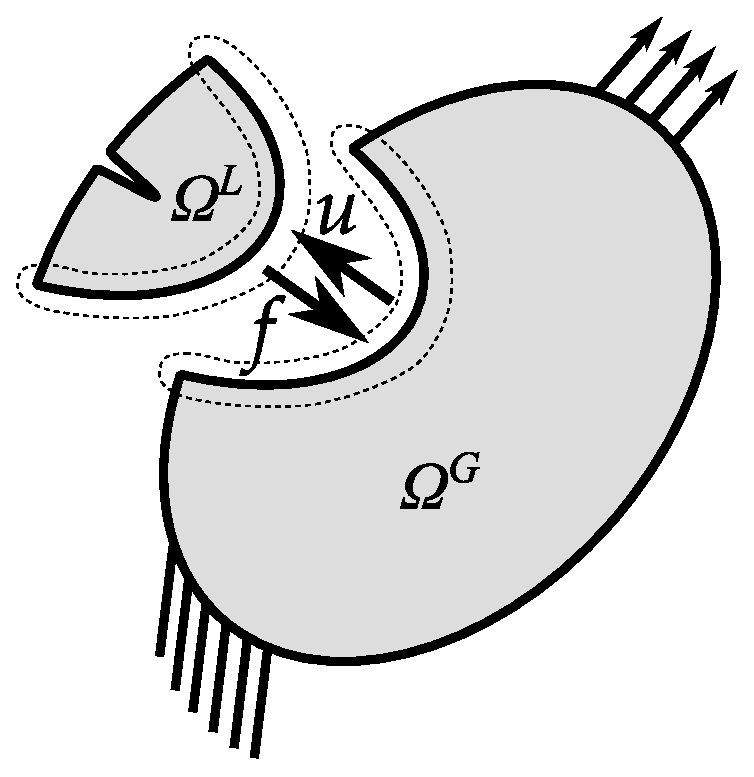
\includegraphics[width=0.5\hsize]{./img/partitioned_iterative.eps}
 \end{center}
 \caption{ʬΥȿ����ˡ�Υ�ǥ�ʬ��ȶ������ʪ���̤μ����Ϥ�}\label{fig:partitioned_iterative}
\end{figure}
\subsection{Aitken �䳰�ˤ��ưŪ����}
�֥��å� Gauss--Seidel ˡ�Ǥϡ�
�����������С��� SOR (Successive Over-relaxation) ˡ�Τ褦�˴��¤�Ԥ����ȤǼ�«���®�����뤳�Ȥ���ǽ�Ǥ��롣
�ܸ���Ǥϡ�
�������Х��ΰ褫����������ΰ�ض����Ѱ̤�����Ϥ��Ȥ��˴��¤�Ԥ���
���ΤȤ���
���·���$\omega$�����ˤ���Ϳ���Ƥ⤢�����٤β�®�������뤬��
���ʤ��«�β�®�Τ�����ܸ���Ǥ�ľ��õ��\cite{Minami2010}���Ѥ��ƴ��·�����ưŪ�˵��롣
ľ��õ���μ�ˡ�Ȥ��Ƥ� Aitken �䳰
\begin{equation}
 \omega^{ (k)} = - \omega^{ (k-1)}
  \frac{
  \bvec{r}^{ (k-1)\trp}
  \left(\bvec{r}^{ (k)} - \bvec{r}^{ (k-1)}\right)}{
  || \bvec{r}^{ (k)} - \bvec{r}^{ (k-1)} ||^2}
\end{equation}
���Ѥ��롣
�����ǡ�$\bvec{r}$�ϻĺ��٥��ȥ�Ǥ��롣
�ޤ������·���$\omega^{(k)}$�ν����$\omega^{(0)}$��\cite{Suzuki1999}����ä�0.1�Ȥ�����

�ʾ��ޤȤ�ơ�
Aitken �䳰�դ��Υ֥��å� Gauss--Seidel ˡ�μ�����
\begin{algorithmic}
 \STATE $k \leftarrow 0$
 \STATE $\omega^{(0)} \leftarrow 0.1$
 \STATE $\bvec{u}^{(0)} \leftarrow \bvec{0}$
 \STATE $\bvec{f}^{(0)} \leftarrow \bvec{0}$
 \STATE $\tilde{\bvec{u}}^{(0)} \leftarrow K_G \left(\bvec{f}^{(0)}\right)$
 \STATE $\bvec{r}^{(0)} \leftarrow - \tilde{\bvec{u}}^{(0)}$
 \WHILE{$||\bvec{r}^{(k)}|| / ||\bvec{r}^{(0)}|| > \tau$}
 \STATE $\bvec{f}^{(k+1)} \leftarrow K_L \left(\bvec{u}^{(k)}\right)$
 \STATE $\tilde{\bvec{u}}^{(k+1)} \leftarrow K_G \left(\bvec{f}^{(k+1)}\right)$
 \STATE $\bvec{r}^{(k+1)} \leftarrow \bvec{u}^{(k)} - \tilde{\bvec{u}}^{(k+1)}$
 \STATE $\omega^{(k+1)} \leftarrow - \omega^{(k)}
 \frac{
 \bvec{r}^{(k)\trp} \left(\bvec{r}^{(k+1)} - \bvec{r}^{(k)}\right)}{
 || \bvec{r}^{(k+1)} - \bvec{r}^{(k)} ||^2}$
 \STATE $\bvec{u}^{(k+1)} \leftarrow \bvec{u}^{(k)} - \omega^{(k+1)} \bvec{r}^{(k+1)}$
 \STATE $k \leftarrow k + 1$
 \ENDWHILE
\end{algorithmic}
�Τ褦�ˤ�����
���������Ÿ�β��ϥ��ƥå���˹Ԥ���
�����ǡ�$\bvec{f}$���ΰ趭����βٽť٥��ȥ롢
$\tilde{\bvec{u}}$��$\bvec{u}$�Ϥ��줾������������¸���ΰ趭������Ѱ̥٥��ȥ�Ǥ��롣
$K_G$���ΰ趭����βٽ�$\bvec{f}$�򶭳����Ȥ��Ʋ��Ϥ�Ԥ���
�ΰ趭������Ѱ�$\bvec{u}$����Ϥ���ؿ��Ǥ��롣
$K_L$��$K_G$��Ʊ�ͤˡ�
�����Ѱ�$\bvec{u}$�����ϤȤ���ȿ��$\bvec{f}$����Ϥ���ؿ��Ǥ��롣
$\bvec{r}$���ΰ趭����λĺ��٥��ȥ롢
$\tau$�ϵ��Ƹ�����$\omega$�ϴ��·����Ǥ��롣
���Ƹ���$\tau$��$10^{-3}$�Ȥ��롣
\section{�������Х��ΰ�������������ϥ���С��μ���}
\subsection{�󼡸������������ϥ���С��μ���}
�ܸ���Ǥϡ�
ʬΥȿ����ˡ�ˤ���˲��ϳإ��ߥ�졼��������Ȥ������Ū�����Ϥ��󼡸����ϤȻ��������Ϥ�Ԥ���
�ܼ�ˡ���������������뤹�뤳�Ȥ򼨤���
�󼡸����ϤǤ��絬�ϲ��Ϥ�ɬ�ܻ���Ǥ�������׻���ԤʤäƤ��ʤ�����
�ܼ�ˡ�Υۥåȥ��ݥåȤ����Τˤ��뤿����󼡸����Ϥμ����ˤĤ��Ƥ��������롣

�������Х��ΰ�Ǥ�ͭ������ˡ�ˤ��ɸ��Ū�������������Ϥ�Ԥ���
ͭ�����Ǥϻ�����ʬ�˴�Ť�ʿ�̱��ϥ������ѥ��ȥ�å����ѷ������ǤȤ���
���������Ŵ�ݤ����ꤷ�ƥ��Ψ 210 GPa���ݥ������� 0.3 �Ȥ��롣
���ơ�Non-overlapping ����ʬΥȿ����ˡ�˴�Ť�������Ÿ�Ǥϡ�
�������Х��ΰ�Ϥ�����ޤޤʤ����ᡢ
�������Х��ΰ�ι�������Ϥ�����Ÿ�������Τ��̤��ư���Ǥ��롣
ľ��ˡ���������դ�ȿ��ˡ�ʤɤ�¿���������������С��Ǥϡ�
����������Ф��Ʋ�������Ԥ��ʳ��ȱ��ե٥��ȥ��Ϳ�����Ȥ���̤�Υ٥��ȥ������ʳ�����Ĥ�ʬ�����\cite{Oguni1991, Davis2006, Saad2003}��
�ܸ���Ǥϡ�ľ��ˡ�ΰ�ĤǤ��� LDL ʬ��ˡ���Ѥ��롣
LDL ʬ��ˡ�ˤ����ơ�
��Ĥ��ʳ��ΰ���ܤ�������Τ� LDL ʬ�� (����ʬ��) �Ǥ��ꡢ
����ܤ�������Τ����ʡ��������� (���ѵ��) �Ǥ��롣
�����ˤĤ��Ƥϲ��ϤΥۥåȥ��ݥåȤǤ��뤿�ᡢ��˾ܺ٤˽Ҥ٤롣
�ܸ���Ǥϡ�
������Ÿ���ϤΤϤ���˥������Х��ΰ�ι����������������� LDL ʬ���Ԥ���
�������Х��ΰ�β�����Ǥ����ʡ����������Τߤ򷫤��֤��褦�ʼ����Ȥ��롣
Ϣ�����ϼ�ˡ�����ʬΥ��ȿ����ˡ�ϡ�
���η���ˡ����Ӥ��ơ�
ȿ�������ʬ����ϢΩ�켡��������;ʬ�˲򤫤ʤ���Фʤ�ʤ�����׻����֤ˤ����ư��̤������Ǥ��롣
�������ʤ��顢
���꤬�����Ǥ���ȿ����ǹ��󤬰���Ǥ���С�
����ܤ�ȿ���ʹߤ�ϢΩ�켡�������ε������ʡ����������ΤߤȤʤ롣
�Ĥޤꡢ�׻����֤�ñ���ȿ������ܤˤʤ�櫓�ǤϤʤ���
���η���ˡ��ʬΥ��ȿ����ˡ�η׻����֤κ��Ϥ����ޤ��礭���ʤ�ʤ���
����ˡ�
������Ÿ���Ϥ�ʸ̮�Ǥ�ʬΥ��ȿ����ˡ��������®�ˤʤꤦ�롣
�Ȥ����Τ⡢
���̤β�����ˡ�ǤϤ�������Ÿ���뤿�Ӥ˥�å����Ѳ����뤿�ᡢ
�����٤˹�������κ���������� LDL ʬ���Ԥ�ɬ�פ����롣
������
ʬΥ��ȿ����ˡ�Ǥϥ������Х��ΰ�Ϥ�����ޤޤʤ����ᡢ
�������Х��ΰ�ι����������������� LDL ʬ��ϲ��ϤΤϤ���˰��Ԥ������Ǥ��롣
ʬΥ��ȿ����ˡ���Ѥ����ϢΩ�켡��������򤯲����¿���ʤ뤬��
���η���ˡ����ʬΥ��ȿ����ˡ��������®�ʥ���С��Ȥʤ뤳�Ȥ����ꤦ�롣

�ܸ���Ǥϰʾ�Τ褦�������������С���ʬΥ��ȿ����ˡ���������ɤ�����Ѥ��ơ�
���η���ˡ�����®�ˤ�����Ÿ���Ϥ�Ԥ���
�����ǡ�
�׻����֤δ����ǽ��פȤʤ������������С��μ����ˤĤ��ƽҤ٤롣
�ܸ���Ǥϡ������������С��� LDL ʬ��ˡ����롣
����Υե����ޥåȤϿ�\ref{fig:skyline}�Τ褦�ʥ������饤��ˡ���Ѥ��롣
��ư������������\texttt{val}��������ʬ���͡�
��ͳ�ٿ�Ĺ����������\texttt{ind}������κǾ��ι��ֹ桢
��ͳ�ٿ�Ĺ����������\texttt{ptr}��\texttt{val}��ι����г���ʬ�����󥤥�ǥå����Ǥ��롣
�������饤��ˡ�Ǥ� LDL ʬ��ϰ���Ū�����ѷ��䳰�ѷ��Υ��르�ꥺ��Ȥϰۤʤꡢ
����Ϣ³����������ô�ݤ�̵�̤ʾ��ʬ�����ӽ��Τ���
\begin{algorithmic}
 \FOR{$k = 0$, $N - 1$}
 \FOR{$i = \mathrm{ind}_k$, $k - 1$}
 \FOR{$j = \max (\mathrm{ind}_k, \mathrm{ind}_i)$, $i - 1$}
 \STATE $\mathrm{val}_{\mathrm{ptr}_k - k + i}
 \leftarrow \mathrm{val}_{\mathrm{ptr}_k - k + i}
 - \mathrm{val}_{\mathrm{ptr}_i - i + j}
 \mathrm{val}_{\mathrm{ptr}_k - k + j}
 \mathrm{val}_{\mathrm{ptr}_j}$
 \ENDFOR
 \STATE $\mathrm{val}_{\mathrm{ptr}_k - k + i}
 \leftarrow \mathrm{val}_{\mathrm{ptr}_k - k + i}
 / \mathrm{val}_{\mathrm{ptr}_i}$
 \STATE $\mathrm{val}_{\mathrm{ptr}_k}
 \leftarrow \mathrm{val}_{\mathrm{ptr}_k}
 - \mathrm{val}_{\mathrm{ptr}_k - k + i}^2
 \mathrm{val}_{\mathrm{ptr}_i}$
 \ENDFOR
 \ENDFOR
\end{algorithmic}
�Τ褦�ʱ��귿�μ����Ȥ���\cite{Oguni1991}��
�����ǡ�$N$�ϼ�ͳ�ٿ���
��ư������������$\mathrm{val}$����������$\mathrm{ind}$��
�������������$\mathrm{ptr}$�ϥ������饤��ˡ������Ǥ��롣
LDL ʬ��β�����޼�����ȿ�\ref{fig:skyline_factorization}�Τ褦�ˤʤ롣
�������饤��ˡ�Ͽ�\ref{fig:skyline}�ξ廰����ʬ���ԻԤι��إӥ뷲�˻��Ƥ��뤿���̿̾������
�������饤��ˡ�Ǥ� LDL ʬ��Ͽ�\ref{fig:skyline_factorization}�Τ褦�˲�������ʬ�ǹͤ��롣

�������饤��ˡ�Ǥ����ʡ����������ϡ�
�����Ϣ³����������ô�ݤ���褦�˼��������
\begin{algorithmic}
 \STATE $\bvec{y} \leftarrow \bvec{f}$
 \FOR{$i = 0$, $N - 1$}
 \FOR{$j = \mathrm{ind}_i$, $i - 1$}
 \STATE $y_i \leftarrow y_i - \mathrm{val}_{\mathrm{ptr}_i - i + j} y_j$
 \ENDFOR
 \ENDFOR
 \FOR{$i = 0$, $N - 1$}
 \STATE $y_i \leftarrow y_i / \mathrm{val}_{\mathrm{ptr}_i}$
 \ENDFOR
 \STATE $\bvec{u} \leftarrow \bvec{y}$
 \FOR{$j = N - 1$, $0$, $-1$}
 \FOR{$i = j - 1$, $\mathrm{ind}_j$, $-1$}
 \STATE $u_i \leftarrow u_i - \mathrm{val}_{\mathrm{ptr}_j - j + i} u_j$
 \ENDFOR
 \ENDFOR
\end{algorithmic}
�Τ褦�ˤʤ롣
�����ǡ�
$\bvec{f}$�ϱ��ե٥��ȥ롢$\bvec{u}$��̤�Υ٥��ȥ롢
$\bvec{y}$�ϼ�ͳ�ٿ�Ĺ�κ���ѥ٥��ȥ�Ǥ��롣
���������ϰ�����¦�Υ롼�פǥ����Ʊ�����$y_i$�˽񤭹��ि������ɤ߹��ߤ�¿�������Ǥ��ꡢ
���������ϵդ˥���񤭹��ߤ�¿�������Ǥ��롣
�󼡸����ϤʤΤǹ���ΥХ������$N^{1/2}$�����㤹��Ȳ��ꤹ��ȡ�
LDL ʬ��α黻�̤�$\mathrm{O} (N^2)$��
���ʡ����������α黻�̤�$\mathrm{O} (N^{3/2})$�Ȥʤꡢ
LDL ʬ��������׻����֤��礭���ʤ뤳�Ȥ�¿����
\begin{figure}[tbp]
 \begin{center}
  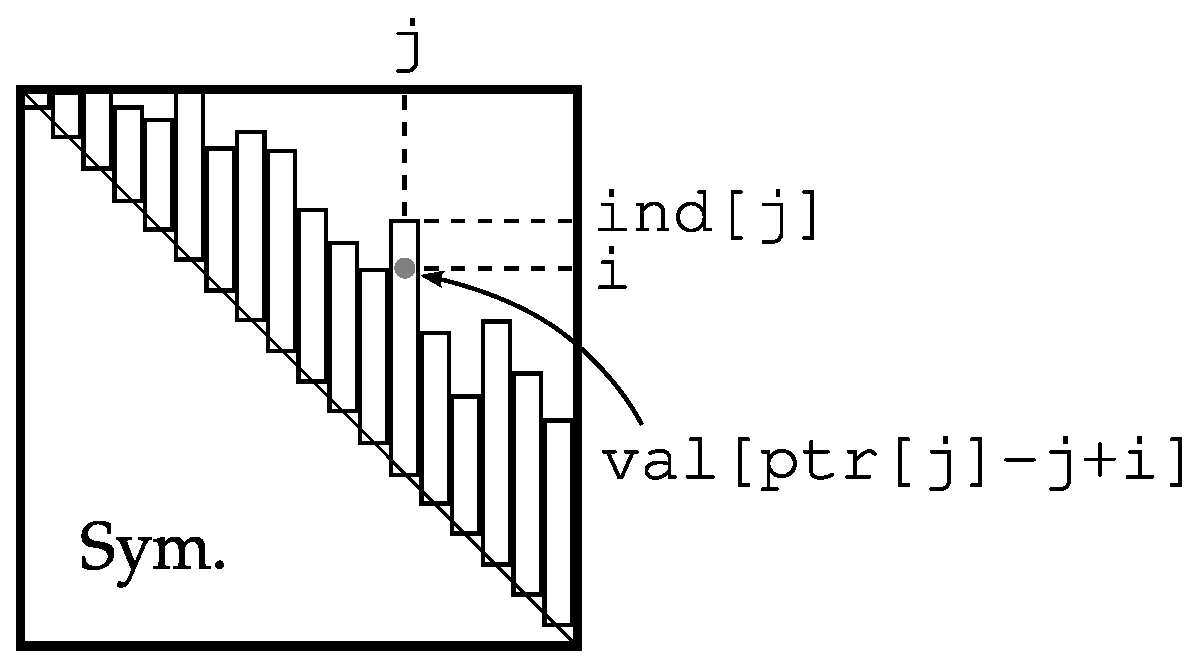
\includegraphics[width=0.8\hsize]{./img/skyline.eps}
 \end{center}
 \caption{�������饤��ˡ�ˤ�뷸������Υǡ�����¤}\label{fig:skyline}
\end{figure}
\begin{figure}[tbp]
 \begin{center}
  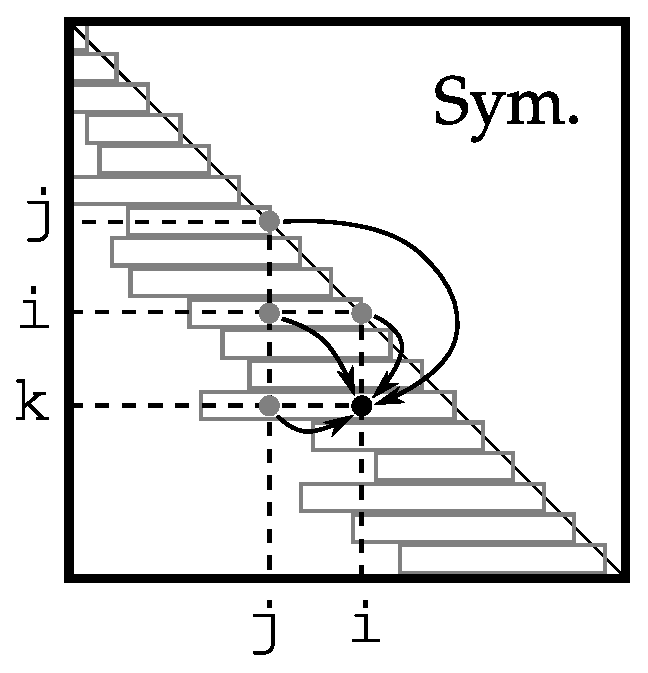
\includegraphics[width=0.42\hsize]{./img/skyline_factorization.eps}
 \end{center}
 \caption{�������饤��ˡ�� LDL ʬ��}\label{fig:skyline_factorization}
\end{figure}
\subsection{�����������������ϥ���С��μ���}
���������ϤǤϻ�����ʬ�˴�Ť��������ѥ��ȥ�å������������Ǥ��Ѥ���
����ʳ����󼡸����Ϥ�Ʊ�ͤȤ��롣
�����������С��ˤ϶�ͭ����������¹���ľ��ˡ����С��Ǥ��� Intel MKL 10.2~\cite{Intel_MKL} �� PARDISO~\cite{Schenka2001} ���Ѥ��롣
PARDISO �ˤ������¹���Υǡ�����¤�Ͽ�\ref{fig:csr}�Τ褦�ʾ廰����ʬ�Τߤ� CSR (Compressed Sparse Row) �ե����ޥåȤǤ��롣
��ư������������\texttt{val}��������󥼥���ʬ���͡�
��������\texttt{ind}���б�����\texttt{val}�����ֹ桢
��������\texttt{ptr}��\texttt{val}�����\texttt{ind}����ι����г���ʬ�����󥤥�ǥå����Ǥ��롣
�ޤ����¹���ľ��ˡ����С��ˤ����ơ�
����������Ф��Ʋ�������Ԥ��ʳ��ϥ���ܥ�å�ʬ�򤪤�ӿ���ʬ��
���ե٥��ȥ��Ϳ�����Ȥ���̤�Υ٥��ȥ������ʳ��ϻ��ѵ��Ǥ��롣
PARDISO �Υ���ܥ�å�ʬ��Ǥϡ�
�ե��륤��ο���Ǿ�������Ǿ��������ˡ\cite{Davis2006}�ˤ�륪������󥰤��Ѥ��Ƥ��롣
�ե��륤��ȤϹ������ʬ�Τ�����
����ʬ�����󥼥��ˤʤ를����ʬ�Τ��ȤǤ��롣
����ʬ��� LDL ʬ��Ǥ��롣
���������ϤʤΤǹ���ΥХ������$N^{2/3}$�����㤹��Ȳ��ꤹ��ȡ�
LDL ʬ��α黻�̤�$\mathrm{O} (N^{7/3})$��
���ʡ����������α黻�̤�$\mathrm{O} (N^{5/3})$�Ȥʤ롣
\begin{figure}[tbp]
 \begin{center}
  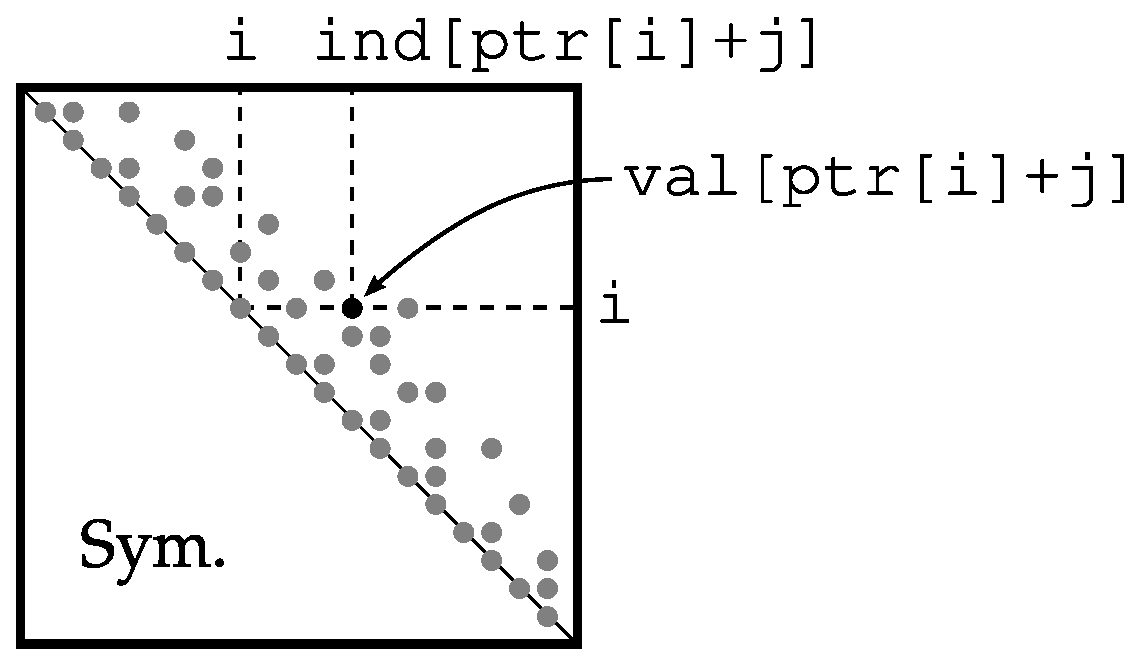
\includegraphics[width=0.75\hsize]{./img/csr.eps}
 \end{center}
 \caption{�廰����ʬ�Τߤ� CSR �ե����ޥåȤη�������Υǡ�����¤}\label{fig:csr}
\end{figure}
\section{���������ΰ�Τ�����Ÿ���ϥ���С��μ���}
���������ΰ�Τ�����Ÿ���ϥ���С��μ����ˤĤ��ƽҤ٤롣
���������ΰ�Ǥϴ���Ū�˥������Х��ΰ��Ʊ�������������С����Ѥ��Ƥ��롣
���ơ�ʬΥȿ����ˡ�ˤ����ơ�
���������ΰ�Υ���С��μ����ǽ��פȤʤ�ΤϹ����������������륿���ߥ󥰤Ǥ��롣
ʬΥȿ����ˡ�Ǥϡ�
������Ÿ�β��ϥ��ƥåפȲ��ϥ��ƥå����ʬΥȿ������ŤΥ롼�׹�¤�ˤʤäƤ��롣
������Ǥ������Ÿ������Τϲ��ϥ��ƥåפ��ʤ���Ȥ��Ǥ��ꡢ
���ϥ��ƥåפ��ʤ�������������������������������������ο���ʬ���Ԥ���
������Ÿ������μ�ͳ�ٿ���ǥ��ꥯ�춭�������Ѳ���ȼ�����ᡢ
��������κ��������ˤϥ���κƳ��ݤ�Ԥ�ɬ�פ����롣

ʬΥȿ����Ǥϥ��������ΰ�ι�����������ѤǤ��뤬��
���������ΰ����Ϳ����붯���Ѱ̶������ (�ǥ��ꥯ�춭�����) ��ȿ�����ƥå�����Ѳ����롣
ʬΥȿ����ˡ�Ǥ��ΰ���˰ۤʤ������������С����Ѥ��뤳�Ȥ���ǽ�Ǥ��뤬��
�ܸ���Ǥϴ�ñ�Τ���˥������Х��ΰ��Ʊ�������������С����Ѥ��Ƥ��롣
�����ǡ�
�����Ǥϥ������饤��ե����ޥåȤ���� CSR �ե����ޥåȤΥǥ��ꥯ�춭�����ν����ˤĤ��ƽҤ٤롣
�ǥ��ꥯ�춭�����ν����ˤϡ�
�ִ�������Ѥ����ǥ��ꥯ�춭�����μ�ͳ�٤�ʬΥ��ԤʤäƤ��롣
�������饤��ե����ޥåȤϹ���ξ廰����ʬ�ˤ�������ͥ��ʤΤǡ�
��������$\bvec{K}$ ($\bvec{K}_L$)��
�ٽť٥��ȥ�$\bvec{f}$ ($\bvec{f}_L$)��
������Ѱ̥٥��ȥ�$\bvec{u}$ ($\bvec{u}_L$) ���ִ�����$\bvec{P}$�ˤ�äƥǥ��ꥯ�켫ͳ�٤���¦��ʬΥ�����
\begin{equation}
 \bvec{P} \bvec{K} \bvec{P}\trp
  = \pmat{
  \begin{array}{cc}
   \bvec{K}_N & \bvec{K}_{ND} \\
   \bvec{K}_{ND}\trp & \bvec{K}_D \\
  \end{array}
  },
\end{equation}
\begin{equation}
 \bvec{P} \bvec{f}
  = \pvec{
  \begin{array}{c}
   \bvec{f}_N \\
   \bvec{f}_D \\
  \end{array}
  } = \pvec{
  \begin{array}{c}
   \bvec{f}_N \\
   \bvec{0} \\
  \end{array}
  },
\end{equation}
\begin{equation}
 \bvec{P} \bvec{u}
  = \pvec{
  \begin{array}{c}
   \bvec{u}_N \\
   \bvec{u}_D \\
  \end{array}
  }
\end{equation}
�Τ褦�ˤʤ롣
�����ǡ�$\bvec{K}_N$�ϥΥ��ޥ�ͳ�٤˴ؤ����������
$\bvec{K}_D$�ϥǥ��ꥯ�켫ͳ�٤˴ؤ����������
$\bvec{K}_{ND}$�ϥΥ��ޥ�ͳ�٤ȥǥ��ꥯ�켫ͳ�٤�������ͳ�٤��ӤĤ����������
$\bvec{u}_N$�ϥΥ��ޥ�ͳ�٤˴ؤ���̤�Τ��Ѱ̥٥��ȥ롢
$\bvec{u}_D$�ϥǥ��ꥯ�켫ͳ�٤˴ؤ�����Τ��Ѱ̥٥��ȥ롢
$\bvec{f}_N$�ϥΥ��ޥ�ͳ�٤˴ؤ���ٽť٥��ȥ롢
$\bvec{f}_D$�ϥǥ��ꥯ�켫ͳ�٤˴ؤ���ٽť٥��ȥ�Ǥ��롣
$\bvec{f}_D$�ϥ����Ǥ��롣
�ޤ����ִ�����$\bvec{P}$�ϼ�ͳ�ٿ�Ĺ����������Ǽ�������롣
�������äơ�
ϢΩ�켡������
\begin{equation}
 \bvec{P} \bvec{K} \bvec{P}\trp
  \bvec{P} \bvec{u}
  = \bvec{P} \bvec{f}
\end{equation}
��
\begin{equation}
 \pmat{
  \begin{array}{cc}
   \bvec{K}_N & \bvec{K}_{ND} \\
   \bvec{K}_{ND}\trp & \bvec{K}_D \\
  \end{array}
  } \pvec{
  \begin{array}{c}
   \bvec{u}_N \\
   \bvec{u}_D \\
  \end{array}
  } = \pvec{
  \begin{array}{c}
   \bvec{f}_N \\
   \bvec{0} \\
  \end{array}
  }
\end{equation}
�Τ褦�ˤʤ롣
������Ф��ƥǥ��ꥯ�춭�����ν�����Ԥ���
\begin{equation}
 \pmat{
  \begin{array}{cc}
   \bvec{K}_N & \bvec{K}_{ND} \\
   \bvec{0} & \bvec{I} \\
  \end{array}
  } \pvec{
  \begin{array}{c}
   \bvec{u}_N \\
   \bvec{u}_D \\
  \end{array}
  } = \pvec{
  \begin{array}{c}
   \bvec{f}_N \\
   \bvec{u}_D \\
  \end{array}
  }
\end{equation}
�Ȥʤꡢ
�ǥ��ꥯ�켫ͳ�٤�õ���
\begin{equation}
 \bvec{K}_N \bvec{u}_N = \bvec{f}_N - \bvec{K}_{ND} \bvec{u}_D
\end{equation}
�Τ褦�ˤʤ롣
�����ǡ�$\bvec{I}$��ñ�̹���Ǥ��롣
���Ū�˥Υ��ޥ�ͳ�٤Τߤ�ϢΩ�켡��������򤱤��ɤ����Ȥˤʤ롣
������
CSR �ե����ޥåȤˤĤ��Ƥ⥹�����饤��ե����ޥåȤȤޤä���Ʊ������Ƴ����뤬��
CSR �ե����ޥåȤϹ���ξ廰����ʬ�ˤ����ƹ�ͥ��ʤΤ�
\begin{equation}
 \bvec{P} \bvec{K} \bvec{P}\trp
  = \pmat{
  \begin{array}{cc}
   \bvec{K}_D & \bvec{K}_{ND}\trp \\
   \bvec{K}_{ND} & \bvec{K}_N \\
  \end{array}
  },
\end{equation}
\begin{equation}
 \bvec{P} \bvec{f}
  = \pvec{
  \begin{array}{c}
   \bvec{0} \\
   \bvec{f}_N \\
  \end{array}
  },
\end{equation}
\begin{equation}
 \bvec{P} \bvec{u}
  = \pvec{
  \begin{array}{c}
   \bvec{u}_D \\
   \bvec{u}_N \\
  \end{array}
  }
\end{equation}
�Τ褦�˥ǥ��ꥯ�켫ͳ�٤���¦��ʬΥ����롣
\section{���}
�ܾϤǤϡ��ܸ�����оݤǤ����絬���˲��ϳ��������ħ��Ҥ١�
������Ф�����ϼ�ˡ�Ȥ���ʬΥȿ����ˡ�Υ��르�ꥺ��ȼ����ˤĤ�������������
�ޤ���
�������Х��ΰ褪��ӥ��������ΰ�γƥ���С��μ����ˤĤ�������������

%% -*- coding: euc-jp -*-
\chapter{���ͼ¸��ȹͻ�}
\section{���}
�ܾϤǤϡ�ʬΥȿ����ˡ���Ѥ��ƿ��ͼ¸���Ԥ���
�ޤ���
ñ��ʷ����Υ�ǥ���Ѥ������������Ϥ��̤��ơ�
ʬΥȿ����ˡ��ȿ�������ˤĤ���Ĵ�٤롣
³���ơ�
ʬΥȿ����ˡ���Ѥ����󼡸�����ӻ���������ϫ������Ÿ���Ϥ�Ԥ���
���ΤȤ���
��ӤΤ�����̾��ͭ������ˡ����ӥ����ߥ�ˡ���Ѥ������Ϥ�Ԥ���
�̾��ͭ������ˡ�ȤϷ׻����֤�������١�
�����ߥ�ˡ�Ȥ����٤���Ӥ�Ԥ���
�󼡸�����ӻ������β��Ϥ��̤��ơ�
�ܼ�ˡ���Ѥ��뤳�Ȥ��絬�ϻ��������Ϥ��Ф��Ƹ�ΨŪ�Ǥ��뤳�Ȥ򼨤���
\section{����������}
����ǤϿ�\ref{fig:two_cubes}�Τ褦��ñ�����Ĥ��������Υ�ǥ���Ų��Ϥ��뤳�Ȥ�ʬΥȿ����ˡ�����������Ū�˹ͻ����롣
�����Ѱ̶�����郎��Ϳ����Ƥ��벼���������򥰥����Х��ǥ롢
��Ϳ����Ƥ��ʤ��������������������ǥ�Ȥ��롣
���Ψ�� 210 GPa���ݥ�������� 0.3 �Ǥ��롣
�ޤ���ͭ�����Ǥϥ������ѥ��ȥ�å�ʿ�̤Ҥ��߻��ѷ������ǤȤ��롣
���Υ�ǥ����Ϥ���Ȥ���
�Ϥ���˥������Х��ǥ����Ϥ��ƽ���ĺ�����뤬��
�������Х��ǥ�˲ٽŶ�����郎��Ϳ����Ƥ��ʤ��Τǽ���ĺ��������ȤʤäƤ��ޤ���
�����ǡ������ܤΥ������Х���ϡ�����������Ϥθ塢
�����ܤΥ������Х���Ϥη�̤������ĺ�����롣

�ޤ���
�����դ��֥��å� Gauss--Seidel ˡ�δ��·������Ѳ�������ȿ��������Ѳ��򸫤롣
³���ơ�
����μ�ͳ�ٿ����Ѳ�������ȿ��������Ѳ���ѻ����롣
\begin{figure}[tbp]
 \begin{center}
  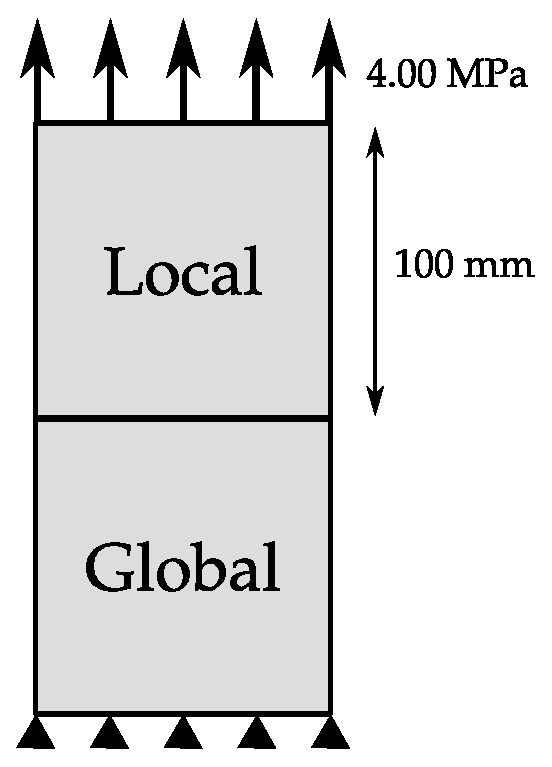
\includegraphics[width=0.4\hsize]{./img/two_cubes.eps}
 \end{center}
 \caption{���������ϥ٥���ޡ����Τ������Ĥ��������Υ�ǥ�}\label{fig:two_cubes}
\end{figure}
\subsection{���·����ˤ��ȿ��������Ѳ�}
�ܾ���Ǥϴ����դ��֥��å� Gauss--Seidel ˡ�δ��·������Ѳ������ơ�
���·����� Aitken �䳰�ˤ��ưŪ�˵�����ˡ��ͭ���Ǥ��뤳�Ȥ򼨤���
�٥���ޡ�������μ�ͳ�٤ϥ������Х��ǥ롢���������ǥ�Ȥ�� 882 ��ͳ�٤Ȥ�����
���������ͳ�٤� 1,764 �Ǥ��롣
���·���$\omega$�� 0.1��0.2��0.3��0.4 ���Ѳ��������Ȥ��ȡ�
Aitken �䳰��ưŪ���¤����Ȥ��ο��ͼ¸���̤��\ref{fig:omega_iter}�˼�����
������ȿ��������ļ����ĺ��Υ��Ǥ��롣
��«���ͤ�$10^{-3}$�Ȥ�����
�ޤ���Aitken �䳰�ν���ͤ�\cite{Suzuki1999}����ä� 0.1 �Ȥ�����
���·���$\omega$�����ˤ���ȳ��ͻĺ���ľ��Ū�˾������ʤ뤳�Ȥ�����դ���狼�롣
�ޤ�������դˤϥץ��åȤ��Ƥ��ʤ���$\omega$��0.5����礭�������ȿ����ȯ������
$\omega = 0.4$�ΤȤ���켡Ū�˼�«�����˼㴳�԰���˼�«���뤳�Ȥ��狼�ä���
����դ��顢
$\omega$����ΤȤ���$\omega = 0.3$�ն�˺�Ŭ��������ȿ�¬�Ǥ��뤬��
����������¸�Ǥ��ꡢ
��ǥ�������Ѳ�����Ⱥ�Ŭ��$\omega$���Ѳ����롣
������Aitken �䳰���Ѥ���ưŪ�ʴ��¤�Ԥ��ȡ�
$\omega$����ΤȤ����⾮����ȿ������Ǽ�«�������롣

���Ʊ������ Aitken �䳰�ν�����·���$\omega_0$��0.0001����0.8�ޤ�Ŭ�����Ѳ��������Ȥ���ȿ�������¬���̤��\ref{fig:omega_zero_iter}�˼�����
������ȿ��������ļ����ĺ��Υ��Ǥ��롣
$\omega_0$�� 0 ���� 1 �δ֤Ǥ���Фۤ�Ʊ��ȿ������Ǽ�«���뤳�Ȥ��狼�ä���
\begin{figure}[tbp]
 \begin{center}
  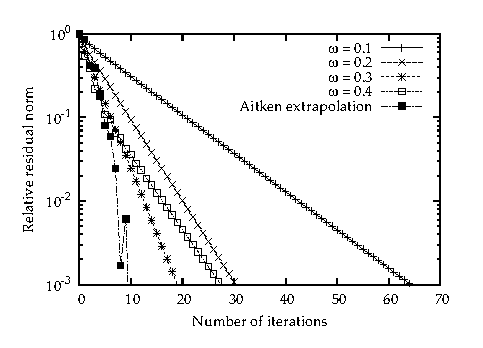
\includegraphics[width=0.9\hsize]{./img/omega_iter/residual.eps}
 \end{center}
 \caption{���·������Ѳ��������Ȥ��μ�«�ĺ�����}\label{fig:omega_iter}
\end{figure}
\begin{figure}[tbp]
 \begin{center}
  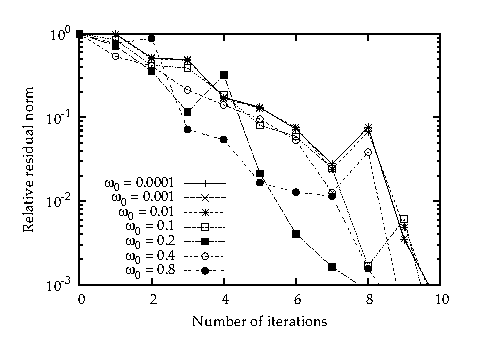
\includegraphics[width=0.9\hsize]{./img/omega_zero_iter/residual.eps}
 \end{center}
 \caption{Aitken �䳰�ν�����·������Ѳ��������Ȥ��μ�«�ĺ�����}\label{fig:omega_zero_iter}
\end{figure}
\subsection{���꼫ͳ�٤ˤ��ȿ��������Ѳ�}
�ܾ���ǤϿ�\ref{fig:two_cubes}�Υ�ǥ������ʬ������Ѳ�������
���구�Ϥ��Ф���ȿ��������Ѳ���Ĵ�٤롣
ɽ\ref{tab:dofs_iter}����������ͳ�٤��Ф���ȿ������򼨤���
��������ͳ�٤˴ؤ�餺����Ʊ��ȿ������Ǽ�«���뤳�Ȥ��狼�ä���
������ǰ����礭����ͳ�٤Ǥ��� 161,604 ��ͳ�٤Υ�å�����\ref{fig:two_cubes_mesh}�ˡ�
���Ϸ�̤��\ref{fig:two_cubes_result}�˼�����
�Ļ벽�ˤϡ�
���ͥ��ߥ�졼������ѲĻ벽�ե졼���� AutoGL~\cite{Kawai2006}���Ѥ�����
�������Х��ΰ�ȥ��������ΰ��Υ���ƲĻ벽���Ƥ��뤬�ºݤˤ�Ϣ³�Ǥ��뤳�Ȥ����դ��롣
���󥿡��� Mises ���������ϤǤ��ꡢ�Ѱ̤� 100 �ܳ��礷�Ƥ��롣
�ޤ������Ϥ��פ������֤�ɽ\ref{tab:rin_spec}�η׻����� 143 s �Ǥ��ä���
\begin{table}[tbp]
 \begin{center}
  \caption{��������ͳ�٤��Ф���ȿ�����}\label{tab:dofs_iter}
  \begin{tabular}{cc|c}
   \hline
   ���դ�����ʬ��� & ����ͳ�� & ȿ����� \\
   \hline
   \hline
   1 & 36 & 6 \\
   2 & 100 & 10 \\
   4 & 324 & 10 \\
   8 & 1,156 & 10 \\
   10 & 1,764 & 10 \\
   20 & 6,724 & 8 \\
   40 & 26,244 & 10 \\
   80 & 103,684 & 10 \\
   100 & 161,604 & 10 \\
   \hline
  \end{tabular}
 \end{center}
\end{table}
\begin{table}[tbp]
 \begin{center}
  \caption{�󼡸����ϤΥ٥���ޡ����˻��Ѥ����׻����Ķ�}\label{tab:rin_spec}
  \begin{tabular}{r|l}
   \hline
   \hline
   CPU  & Intel Core i7-920 (Nehalem) \\
   {}   & 42.7 Gflops \\
   {}   & 2.67 GHz \\
   {}   & 4 cores \\
   {}   & SSE4 \\
   {}   & L2 cache 256 KB $\times$ 4 \\
   {}   & L3 cache 8 MB \\
   {}   & QPI 4.8 GT/s \\
   DRAM & DDR3-1066 \\
   {}   & 12 GB (2 GB $\times$ 6) \\
   {}   & 25.6 GB/s \\
   OS   & Ubuntu 11.04 (Natty Narwhal) \\
   Compiler & Intel C/C++ Compiler 12.1\cite{Intel_Compilers} \\
   \hline
  \end{tabular}
 \end{center}
\end{table}
\section{�󼡸�����ϫ������Ÿ����}
����ǤϿ�\ref{fig:ect}�Τ褦����¦�ˤ����Τ������Ĥ��󼡸�������Ÿ���Ϥ�Ԥ���
���ϥ�������Ȥ��ơ�ʬΥȿ����ˡ��¾�ˡ�
����оݤȤ����̾��ͭ������ˡ����ӥ����ߥ�ˡ���Ѥ��롣
�̾��ͭ������ˡ�ȤϷ׻����֤�������٤���Ӥ���
�����ߥ�ˡ�Ȥ����٤���Ӥ�Ԥ���

�ޤ���ʬΥȿ����ˡ���Ѥ��Ʋ��Ϥ�Ԥ���
���ĥ�ǥ�ξ岼���о������� 2 ʬ�� 1 ��ǥ���������
�������ѥ��ȥ�å�ʿ�̱��ϻ��ѷ������Ǥ��Ѥ���ʬ���Ԥ���
�������Х��ǥ�μ�ͳ�ٿ��� 105,382��
���������ǥ�μ�ͳ�ٿ��������� 8 ʬ�� 1 �� 13,702��
����ͳ�ٿ��� 119,084 �Ǥ��롣
���Ψ�� 210 GPa���ݥ�������� 0.3 �Ǥ��롣
������Ÿ���Ϥβ��ϥ��ƥå׿��ϡ�
����Ĺ$a$�� 10.0 mm ���� 14.0 mm �ޤǰ����Ǥ��Ŀ�Ÿ�������� 41 ���ƥåפǤ��롣
����Ĺ$a$�� 10.0 mm �ΤȤ��Υ�å�����\ref{fig:ect_2d_mesh}�ˡ�
���ϥ��󥿡�������ѷ��ޤ��\ref{fig:ect_2d_result}�˼�����
���ϥ��󥿡��� Mises ���������ϤǤ��ꡢ�Ѱ̤� 100 �ܤ˳��礷�Ƥ��롣
�������Х��ǥ�ȥ��������ǥ��ʬΥ���ƲĻ벽���Ƥ��뤳�Ȥ����դ��롣
��\ref{fig:ect_2d_residual}�˲��Ϥκǽ�� 10 ���ƥå�ʬ�λĺ�����򼨤���
��������ȿ��������ļ����ĺ��Υ��Ǥ��롣
��\ref{fig:ect_2d_residual2}�������ϥ��ƥåפ��줾��λĺ������Ťͤ��碌������դ򼨤���
������ȿ��������ļ����ĺ��Υ��Ǥ��롣
��\ref{fig:ect_2d_num_iter}�˳Ʋ��ϥ��ƥåפ�ȿ������򼨤���
���������ϥ��ƥåס��ļ���ȿ������Ǥ��롣
���ϥ��ƥåפϤ���Ĺ���б����뤬��
ȿ������Ϥ���Ĺ�˴ؤ�餺���ޤ��Ѳ����ʤ����Ȥ��狼�ä���
ɽ\ref{tab:rin_spec}�η׻������Ѥ����Ȥ��η׻����֤���Ӥ��ν������������ɽ\ref{tab:ect_2d_time}�˼�����
�߷׷׻����֤�ʣ����Ԥ�������η׻����֤��߷ס�
ʿ�ѷ׻����֤��߷׷׻����֤��������dz�ä���ΤǤ��롣
�ޤ����֤���¾�פν����ϥ�����ݡ��ե����������ϡ���������������ʤɤ�ޤࡣ
³���ơ�Ʊ�ͤβ��Ϥ��̾��ͭ������ˡ�ˤƹԤä���
�׻����֤�ɽ\ref{tab:ect_2d_time_conventional}�˼�����
ɽ\ref{tab:ect_2d_time}��ɽ\ref{tab:ect_2d_time_conventional}����Ӥ���ȡ�
�̾��ͭ������ˡ���Ѥ������ʬΥȿ����ˡ���Ѥ������� 12.9 ��®���ʤä���
�����̤η׻����֤򸫤�ȡ�
�����������Τν����� 8 �䶯�� LDL ʬ�򤪤�����ʡ����������������Ƥ��뤳�Ȥ��狼�롣
�̾��ͭ������ˡ�Ǥ� LDL ʬ�򤪤�����ʡ�������������ϥ��ƥå׿������Ԥ�����
ʬΥȿ����ˡ�Ǥϥ������Х���Ϥ� LDL ʬ��� 1 �󤷤��Ԥ�ʤ���
�����ʬΥȿ����ˡ�ξ�硢�������Х��ǥ뤬������ޤޤʤ�����˥�å��太��ӹ������󤬲������Τ��̤������ѤǤ��뤫��Ǥ��롣
�ޤ���ʬΥȿ����ˡ�Ǥ��̾��ͭ������ˡ�������ʡ����������β����¿���ʤäƤ��롣
����ϳƲ��ϥ��ƥå����ȿ���׻��Ǥ��ꡢ
����β�����ǤϿ�\ref{fig:ect_2d_num_iter}���̤�ʿ�� 15.6 �ܤβ���������ʡ�����������ԤäƤ��롣
����������ͳ�ٿ����礭��ϢΩ�켡�������ξ�硢
���ʡ����������η׻����֤ϰ��̤� LDL ʬ��η׻����֤���Ӥ�������˾��������ᡢ
���Ū��ʬΥȿ����ˡ�������̾��ͭ������ˡ���⾮�����׻����֤ȤʤäƤ��롣
���Τ褦��ʬΥȿ����ˡ��ͥ�����ϡ�
���������ǥ�Τߤǥ�å���ޤ������ǹ������Ѳ�����褦�ʾ��˾�������롣
�ܼ�ˡ�ϡ�
¿���κ������������ݤʤɡ�
�����������ɽ�Ū��ȯ������褦��������̤˱��Ѥ��뤳�Ȥ���ǽ�Ǥ���ȹͤ����롣

ʬΥȿ����ˡ���̾��ͭ������ˡ������ӥ����ߥ�ˡ�����٤���Ӥ��롣
�����ߥ�ˡ�Υ������Х��ǥ�Ǥ�����ʤ���Ƥ���å���ʬ���Ԥ��٤�������
�������Ӥδ�ñ�Τ���˿�\ref{fig:ect_2d_mesh}��Ʊ�ͤκ٤����Υ�å���ʬ���Ԥ���
���Υ�ǥ벽��ˡ�Ǥϡ�
�Ƥ���å��夬�ð۾��ɽ���Ǥ��ʤ����Ȥˤ������������
�������֤ˤ��������������Ĥ��ӽ����Ƥ��롣
���̤˥����ߥ�ˡ�Ǥϡ��������ǥ벽���ʤ�����
�⤷�����Ƥ���å���ǥ�ǥ벽���롣
����Ϥ���Ĺ$a$����Ĺ�� 10.0 mm �����Ÿ��������
���������ǥ�ǤΤߤ������Ÿ������褦�ʥ�ǥ벽��Ԥ���
�ޤ����������Х��ǥ뤫����������ǥ���Ϥ��������Ϥ��٤Ƥ������Ƕ����Ѱ̶������Ȥ��롣
��\ref{fig:ect_2d_result_zooming}�ˤ���Ĺ$a$�� 14.0 mm (�������Х��ǥ�Ǥ� 10.0 mm) �ΤȤ��β��Ϸ�̤򼨤���
��\ref{fig:ect_2d_sif}�˲��Ϸ�̤���ľ���Ѱ̳���ˡ�ˤ���᤿���ϳ��緸���򼨤���
��������¦�ˤ����Τ������Ĥΰ��Ͱ�ĥ��������
\begin{equation}
 K_I = F (a/W) \sigma \sqrt{\pi a},
\end{equation}
\begin{equation}
 F (a/W) = 1.12 - 0.231 (a/W) + 10.55 (a/W)^2 - 21.72 (a/W)^3 + 30.39 (a/W)^4
\end{equation}
�Ǥ���\cite{Shiratori1980}��
��\ref{fig:ect}����$a$�� 10.0 mm ���� 14.0 mm��
$W = 48.0$ mm��$\sigma = 100$ MPa�Ǥ��롣
��\ref{fig:ect_2d_cycles}�˱��ϳ��緸�������᤿��ϫ����������򼨤���
������Ÿ§�ˤϼ� (\ref{eq:paris_law}) �� Paris §���Ѥ�����
����κ�����������ܵ����ز�ȯ���Ѹ������������ʰݻ�����\cite{jsmecode}����$C = 3.78 \times 10^{-12}$��$n = 3.07$�Ȥ���
$\Delta K = K_I$��$\Delta a = 0.1$ mm (����) �Ȥ�����
ʬΥȿ����ˡ�β���̾��ͭ�����Dz��Ϥˤ���᤿��Ȥۤܰ��פ��Ƥ��ꡢ
������Ȥ⤢�����ٰ��פ��Ƥ��뤳�Ȥ��狼�롣
�������ʤ��顢�����ߥ�ˡ�β�Ϥ������礭��Υ��Ƥ��롣
�����ߥ�ˡ�����٤ϥ��������ΰ���礭��������Ϥ����������Ҵ��Ǥ��롣
����β���������٤��������㤫�ä���ͳ�ϡ�
����Ĺ�����������ΰ��Ⱦʬ�ʾ������Ĺ���ä�����Ǥ��롣
�ޤ���
�����Ϥ�������郎���٤ƶ����Ѱ̶������Ǥ��ä��Τ����������˴�Ϳ���Ƥ��롣
�����ߥ�ˡ�Ǥϡ�
����β�����Τ褦�˰�ľ�������Ԥ��Ƚ�ʬ�����٤β�����줺��
��ʬ�����٤β�������褦�ʥ��������ΰ���礭���䶭����������ˤϷи���ɬ�פǤ��롣
\begin{figure}[tbp]
 \begin{center}
  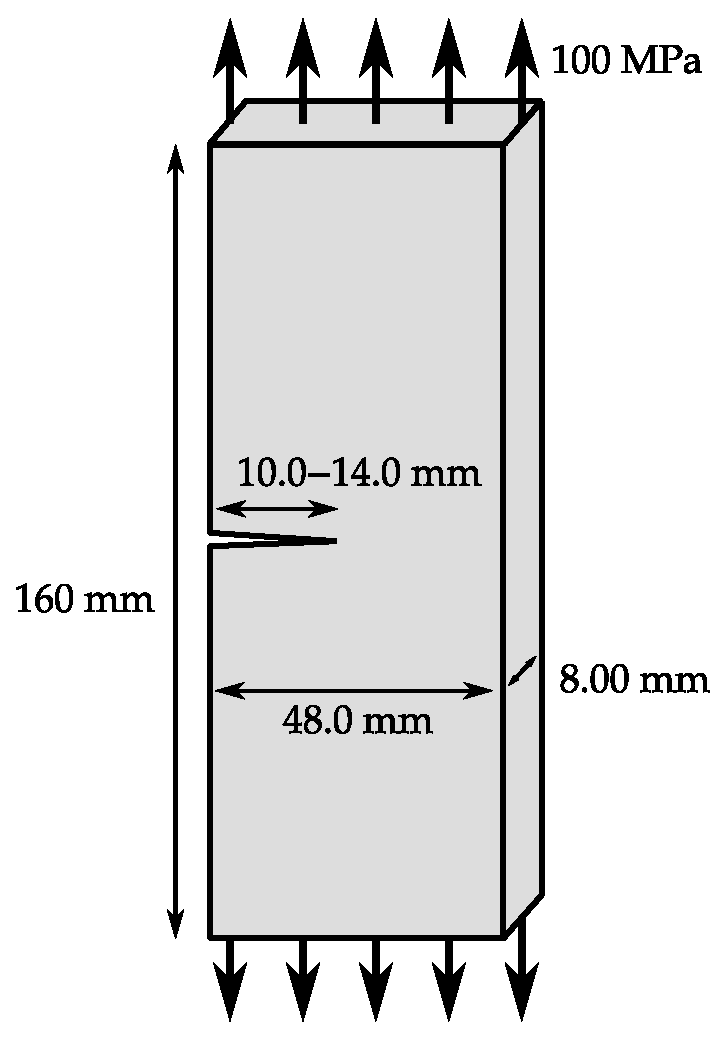
\includegraphics[width=0.5\hsize]{./img/ect.eps}
 \end{center}
 \caption{��¦�ˤ����Τ������Ĥΰ��Ͱ�ĥ}\label{fig:ect}
\end{figure}
\begin{figure}[tbp]
 \begin{center}
  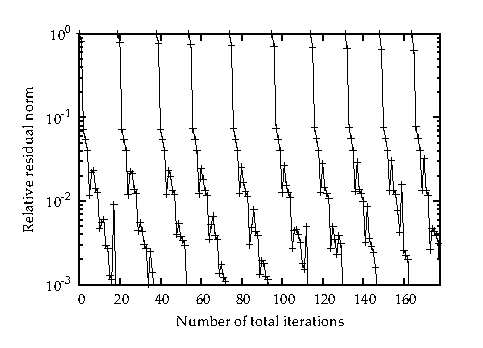
\includegraphics[width=0.9\hsize]{./img/ect_2d/residual/residual.eps}
 \end{center}
 \caption{ʬΥȿ����ˡ�ˤ���󼡸�������Ÿ���Ϥκǽ�� 10 ���ƥåפλĺ�����}\label{fig:ect_2d_residual}
\end{figure}
\begin{figure}[tbp]
 \begin{center}
  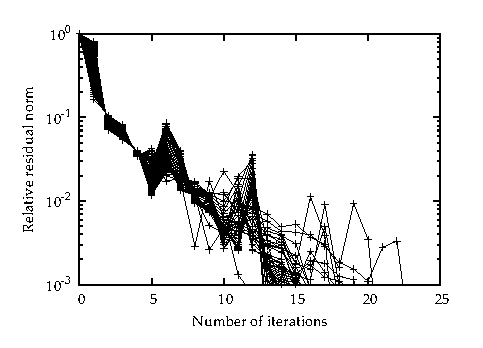
\includegraphics[width=0.9\hsize]{./img/ect_2d/residual/residual2.eps}
 \end{center}
 \caption{ʬΥȿ����ˡ�ˤ���󼡸�������Ÿ���Ϥλĺ�����}\label{fig:ect_2d_residual2}
\end{figure}
\begin{figure}[tbp]
 \begin{center}
  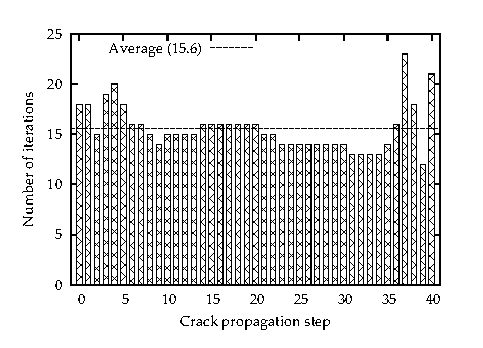
\includegraphics[width=0.9\hsize]{./img/ect_2d/num_iter/num_iter.eps}
 \end{center}
 \caption{ʬΥȿ����ˡ�ˤ���󼡸�������Ÿ���Ϥ�ȿ�����}\label{fig:ect_2d_num_iter}
\end{figure}
\begin{table}[tbp]
 \begin{center}
  \caption{ʬΥȿ����ˡ�ˤ���󼡸�������Ÿ���Ϥη׻����֤Ȥ��ν����������}\label{tab:ect_2d_time}
  \begin{tabular}{r|ccc}
   \hline
   �������� & �߷׷׻����� & ʿ�ѷ׻����� & ������� \\
   \hline
   \hline
   ���� & 878 s & - & - \\
   \hline
   �������Х���Ϥ� LDL ʬ��      & 198 s (23 \%) & 198 s    & 1 \\
   ����������Ϥ� LDL ʬ��        & 411 s (47 \%) & 10.0 s   & 41 \\
   �������Х���Ϥ����ʡ��������� & 118 s (13 \%) & 0.174 s  & 680 \\
   ����������Ϥ����ʡ���������   & 10.7 s (1 \%) & 0.0167 s & 639 \\
   ����¾                         & 140 s (16 \%) & -        & - \\
   \hline
  \end{tabular}
 \end{center}
 \begin{center}
  \caption{�̾��ͭ������ˡ�ˤ���󼡸�������Ÿ���Ϥη׻����֤Ȥ��ν����������}\label{tab:ect_2d_time_conventional}
  \begin{tabular}{r|ccc}
   \hline
   �������� & �߷׷׻����� & ʿ�ѷ׻����� & ������� \\
   \hline
   \hline
   ���� & 11,300 & - & - \\
   \hline
   LDL ʬ��       & 9,180 s (81 \%) & 224 s   & 41 \\
   ���ʡ��������� & 7.41 s (0 \%)   & 0.181 s & 41 \\
   ����¾         & 2,110 s (19 \%) & -       & - \\
   \hline
  \end{tabular}
 \end{center}
\end{table}
\begin{figure}[tbp]
 \begin{center}
  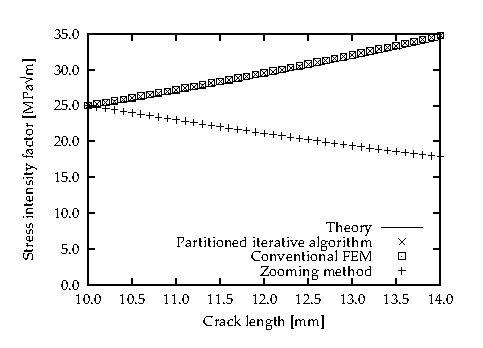
\includegraphics[width=0.9\hsize]{./img/ect_2d/sif/sif.eps}
 \end{center}
 \caption{�󼡸�������Ÿ���Ϥα��ϳ��緸��}\label{fig:ect_2d_sif}
\end{figure}
\begin{figure}[tbp]
 \begin{center}
  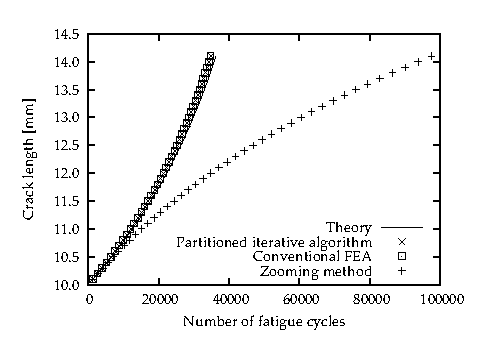
\includegraphics[width=0.9\hsize]{./img/ect_2d/sif/cycles.eps}
 \end{center}
 \caption{�󼡸�������Ÿ���Ϥ���ϫ���������}\label{fig:ect_2d_cycles}
\end{figure}
\section{����������ϫ������Ÿ����}
��\ref{fig:ect}�Υ�ǥ�λ���������ϫ������Ÿ���Ϥ�Ԥä���
�о��������\ref{fig:ect_3d_mesh}�Τ褦�� 4 ʬ�� 1 ��ǥ�Υ�å�������������
ͭ�����Ǥϥ������ѥ��ȥ�å������������ǤǤ��ꡢ
����������󼡸����Ϥ�Ʊ�ͤ˥��Ψ 210 GPa���ݥ������� 0.3 �Ȥ�����
�������Х��ǥ�μ�ͳ�ٿ��� 1,738,803��
���������ǥ�μ�ͳ�ٿ��� 226,083��
����ͳ�ٿ��� 1,964,886 �Ǥ��롣
�׻����Ķ���ɽ\ref{tab:times_spec}�Τ褦�ʰ���η׻����Ǥ��롣
����Ĺ$a$�� 10.0 mm �ΤȤ��β��Ϸ�̤��\ref{fig:ect_3d_result}�˼�����
�Ѱ̤� 200 �ܤ˳��礷�Ƥ��롣
�����������С��ˤ� Intel MKL 10.2~\cite{Intel_MKL} �� PARDISO~\cite{Schenka2001} ���Ѥ���
���󥹥�åɿ��� 4 �Ȥ�����
��������̤ϼ�ͳ�ٿ��˳������㤷����β�����Ǥ� 19.4 GB �Ǥ��ä���
�������̾��ͭ������ˡ�Υ�������̤� 20.9 GB �Ǥ��ä���
ʬΥȿ����ˡ�η׻����֤�ɽ\ref{tab:ect_3d_time}��
�̾��ͭ�����Dz��Ϥη׻����֤�ɽ\ref{tab:ect_3d_time_conventional}�˼�����
�ޤ���ʬΥȿ����ˡ�β��ϥ��ƥå���λĺ�������\ref{fig:ect_3d_residual}����ӿ�\ref{fig:ect_3d_residual2}�ˡ�
ȿ��������\ref{fig:ect_3d_num_iter}�˼�����
��\ref{fig:ect_3d_residual}����ӿ�\ref{fig:ect_3d_residual2}�β�����ȿ�������
�ļ��ϻĺ��Υ��Ǥ��롣
��\ref{fig:ect_3d_num_iter}�β����ϲ��ϥ��ƥåס��ļ���ȿ������Ǥ��롣
ȿ�������ʿ�Ѥ��󼡸����ϤȤۤ��Ѥ�餺��15.8 ��Ǥ��ä���
ξ�Ԥη׻����֤���Ӥ��롣
���ԡ��ɥ��åפ� 4.52 �Ǥ��ä���
�ޤ���ʬΥȿ����ˡ�η׻����֤� 50 \%���̾��ͭ������ˡ�η׻����֤� 11 \% �Ǥ���֤���¾�פ� 6 ���ö��ϥ�����ݡ��ե����������ϡ���������������ʤɤ�ޤࡣ
�äˡ����Τ����� 3 ʬ�� 1 �� 2,100 s �ϲ��ϥ��ƥå���Υե�������ϤǤ��ä���
���Τ褦�ˡ�ʬΥȿ����ˡ�ξ��Ϸ׻����֤� 50 \% ��֤���¾�פ����뤬��
������󼡸����Ϥ�Ʊ�ͤ˥ۥåȥ��ݥåȤ������������С��Ǥ��롣
������󼡸����Ϥ�Ʊ�ͤˡ�
�������Х���ϤΥ���ܥ�å�ʬ�򤪤�ӿ���ʬ�����ϤΤϤ���˰��Ԥ������ˤʤ롣
�����ơ����ѵ��β����ȿ���������¿���ʤ뤬��
���ΤȤ��Ƥ�ʬΥȿ����ˡ�������׻����֤��������ʤ롣

����Ĺ$a = 10.0$ mm �ΤȤ��Τ�����ü�α��ϳ��緸�����\ref{fig:ect_3d_sif_thickness}�˼�����
�������ĸ�������������ɸ���ļ������ϳ��緸���Ǥ��롣
�ʤ���
�ĸ������κ�ɸ����Τ�Τ��о����������Τ�Τ�Ʊ���ͤ��ޤ��֤���ɽ�����Ƥ��롣
����β�����Τ褦���󼡸�Ū�ʤ����Ǥϡ�
�ĸ���ͭ�¤Ǥ��뤳�Ȥ�����ϳ��緸�������οޤΤ褦�˻����ˤʤ뤳�Ȥ��Τ��Ƥ��ꡢ
����β��ϤǤ⤳���Ƹ��Ǥ��Ƥ��롣
�ޤ���
ʬΥȿ����ˡ������̾��ͭ�����Dz��Ϥη�̤��󼡸����Ϥ�Ʊ�ͤ�������Ȥۤܰ��פ��Ƥ��롣

�������Ÿ�������Ȥ��γƿ�Ÿ���ƥåפα��ϳ��緸�����\ref{fig:ect_3d_sif}�˼�����
�Ʋ��ϥ��ƥåפα��ϳ��緸���ˤϿ�\ref{fig:ect_3d_sif_thickness}������κ�ɸ���ͤ��Ѥ��Ƥ��롣
���α��ϳ��緸������ Paris §�ˤ���᤿��ϫ������������\ref{fig:ect_3d_cycles}�˼�����
�󼡸����Ϥ�Ʊ�ͤˡ�
ʬΥȿ����ˡ���̾��ͭ�����Dz��Ϥη�̤��褯���פ��Ƥ��뤳�Ȥ��狼�롣
\begin{table}[tbp]
 \begin{center}
  \caption{���������ϤΥ٥���ޡ����˻��Ѥ����׻����Ķ�}\label{tab:times_spec}
  \begin{tabular}{r|l}
   \hline
   \hline
   CPU  & Intel Core i7-930 (Nehalem) \\
   {}   & 44.8 Gflops \\
   {}   & 2.80 GHz \\
   {}   & 4 cores \\
   {}   & SSE4 \\
   {}   & L2 cache 256 KB $\times$ 4 \\
   {}   & L3 cache 8 MB \\
   {}   & QPI 4.8 GT/s \\
   DRAM & DDR3-1333 \\
   {}   & 24 GB (4 GB $\times$ 6) \\
   {}   & 25.6 GB/s \\
   OS   & Linux Mint 12 (Lisa) \\
   Compiler & Intel C/C++ Compiler 12.1\cite{Intel_Compilers} \\
   \hline
  \end{tabular}
 \end{center}
\end{table}
\begin{figure}[tbp]
 \begin{center}
  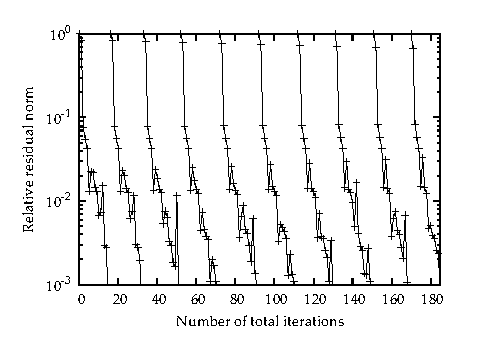
\includegraphics[width=0.9\hsize]{./img/ect_3d/residual/residual.eps}
 \end{center}
 \caption{ʬΥȿ����ˡ�ˤ�뻰����������Ÿ���Ϥκǽ�� 10 ���ƥåפλĺ�����}\label{fig:ect_3d_residual}
\end{figure}
\begin{figure}[tbp]
 \begin{center}
  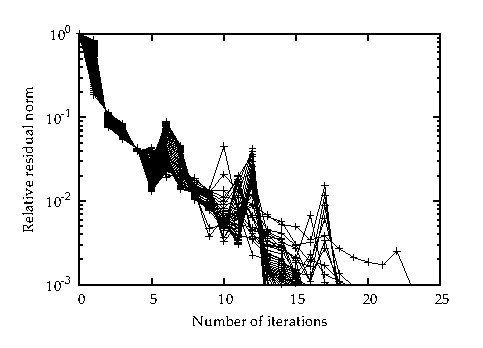
\includegraphics[width=0.9\hsize]{./img/ect_3d/residual/residual2.eps}
 \end{center}
 \caption{ʬΥȿ����ˡ�ˤ�뻰����������Ÿ���Ϥλĺ�����}\label{fig:ect_3d_residual2}
\end{figure}
\begin{figure}[tbp]
 \begin{center}
  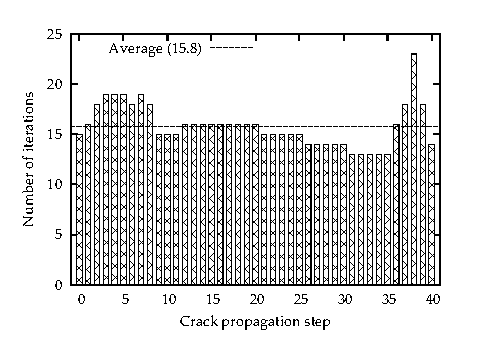
\includegraphics[width=0.9\hsize]{./img/ect_3d/num_iter/num_iter.eps}
 \end{center}
 \caption{ʬΥȿ����ˡ�ˤ�뻰����������Ÿ���Ϥ�ȿ�����}\label{fig:ect_3d_num_iter}
\end{figure}
\begin{table}[tbp]
 \begin{center}
  \caption{ʬΥȿ����ˡ�ˤ�뻰����������Ÿ���Ϥη׻����֤Ȥ��γƽ����������}\label{tab:ect_3d_time}
  \begin{tabular}{r|ccc}
   \hline
   �������� & �߷׷׻����� & ʿ�ѷ׻����� & ������� \\
   \hline
   \hline
   ���� & 12,600 s & - & - \\
   \hline
   �������Х���Ϥ�ʬ�����     & 960 s (8 \%)    & 960 s   & 1 \\
   ����������Ϥ�ʬ�����       & 1,190 s (9 \%)  & 29.0 s  & 41 \\
   �������Х���Ϥλ��ѵ����� & 3,730 s (30 \%) & 5.41 s  & 690 \\
   ����������Ϥλ��ѵ�����   & 407 s (3 \%)    & 0.627 s & 649 \\
   ����¾                       & 6,310 s (50 \%) & -  & - \\
   \hline
  \end{tabular}
 \end{center}
 \begin{center}
  \caption{�̾��ͭ������ˡ�ˤ�뻰����������Ÿ���Ϥη׻����֤Ȥ��γƽ����������}\label{tab:ect_3d_time_conventional}
  \begin{tabular}{r|ccc}
   \hline
   �������� & �߷׷׻����� & ʿ�ѷ׻����� & ������� \\
   \hline
   \hline
   ���� & 57,000 s & - & - \\
   \hline
   ʬ�����     & 50,300 s (88 \%) & 1,230 s & 41 \\
   ���ѵ����� & 257 s (1 \%)     & 6.27 s  & 41 \\
   ����¾       & 6,440 s (11 \%)  & -  & - \\
   \hline
  \end{tabular}
 \end{center}
\end{table}
\begin{figure}[tbp]
 \begin{center}
  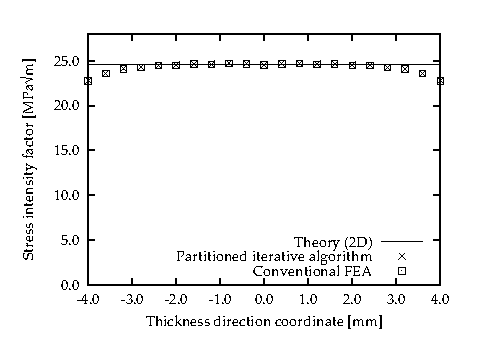
\includegraphics[width=0.9\hsize]{./img/ect_3d/sif/sif_thickness.eps}
 \end{center}
 \caption{��¦�ˤ����Τ������ĤΤ�����ü�α��ϳ��緸��}\label{fig:ect_3d_sif_thickness}
\end{figure}
\begin{figure}[tbp]
 \begin{center}
  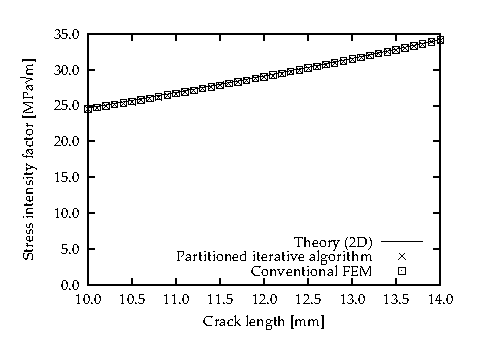
\includegraphics[width=0.9\hsize]{./img/ect_3d/sif/sif.eps}
 \end{center}
 \caption{������������Ÿ���Ϥα��ϳ��緸��}\label{fig:ect_3d_sif}
\end{figure}
\begin{figure}[tbp]
 \begin{center}
  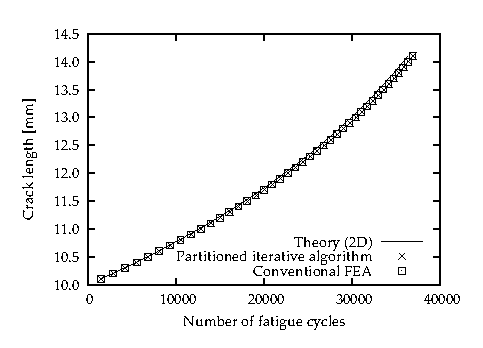
\includegraphics[width=0.9\hsize]{./img/ect_3d/sif/cycles.eps}
 \end{center}
 \caption{������������Ÿ���Ϥ���ϫ���������}\label{fig:ect_3d_cycles}
\end{figure}
\section{���}
�ܾϤǤϡ�ʬΥȿ����ˡ���Ѥ��ƿ��ͼ¸���Ԥä���
�ޤ���
ñ��ʷ����Υ�ǥ���Ѥ������������Ϥ��̤��ơ�
ʬΥȿ����ˡ��ȿ�������ˤĤ���Ĵ�٤���
Aitken �䳰�ˤ��ưŪ�����դ��Υ֥��å� Gauss--Seidel ˡ���Ѥ���С�
������·���������μ�ͳ�ٿ��˴ؤ�餺�ۤܰ����ȿ������Ǽ�«���뤳�Ȥ��狼�ä���
³���ơ�
ʬΥȿ����ˡ���Ѥ����󼡸�����ӻ���������ϫ������Ÿ���Ϥ�Ԥä���
�󼡸��� 12 ����ͳ�٤β�����Ǥ��̾��ͭ������ˡ���� 12.9 �ܡ�
�������� 196 ����ͳ�٤β�����Ǥ� 4.52 �ܹ�®��������
�ޤ������٤��̾��ͭ������ˡ�Ȥۤ�Ʊ���Ǥ��ꡢ
�����ߥ�ˡ�Ȱ�ä����٤����������ΰ���礭���ˤۤȤ�ɰ�¸���ʤ����Ȥ��狼�ä���
\begin{figure}[p]
 \begin{center}
  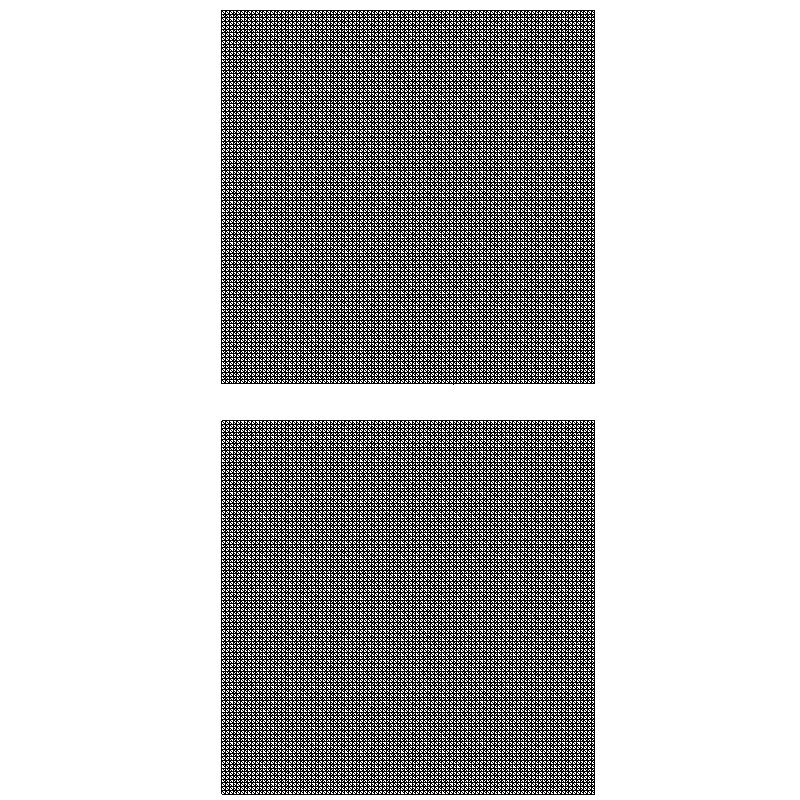
\includegraphics[width=\hsize, bb=0 0 800 800]{./img/two_cubes/mesh.png}
 \end{center}
 \caption{��Ĥ��������Υ�ǥ�� 16 ����ͳ�٤Υ�å���}\label{fig:two_cubes_mesh}
\end{figure}
\begin{figure}[p]
 \begin{center}
  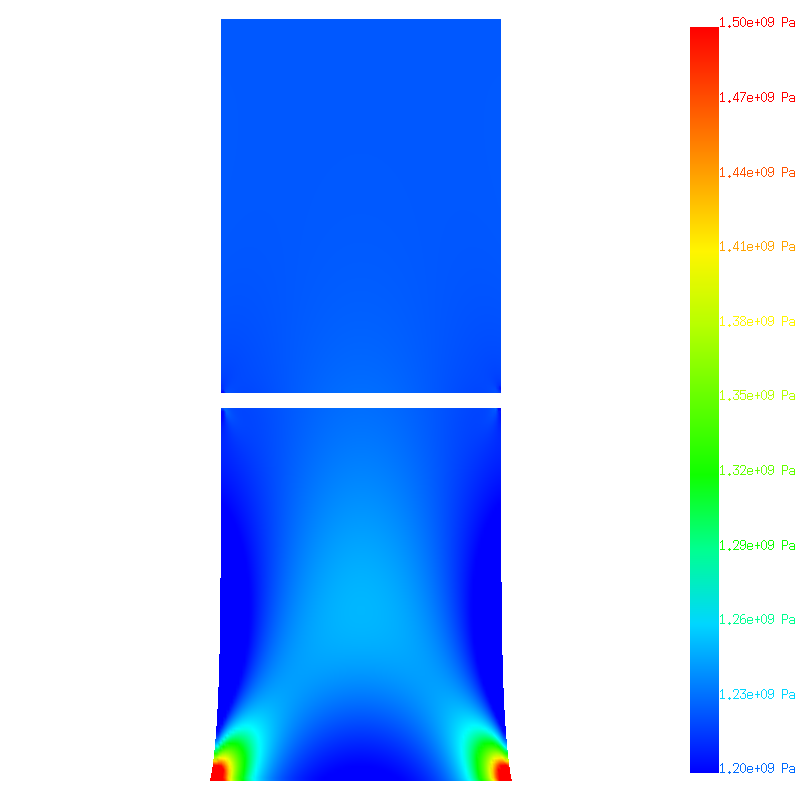
\includegraphics[width=\hsize, bb=0 0 800 800]{./img/two_cubes/result.png}
 \end{center}
 \caption{��Ĥ��������Υ�ǥ�α��ϥ��󥿡��դ��ѷ���}\label{fig:two_cubes_result}
\end{figure}
\begin{figure}[p]
 \begin{center}
  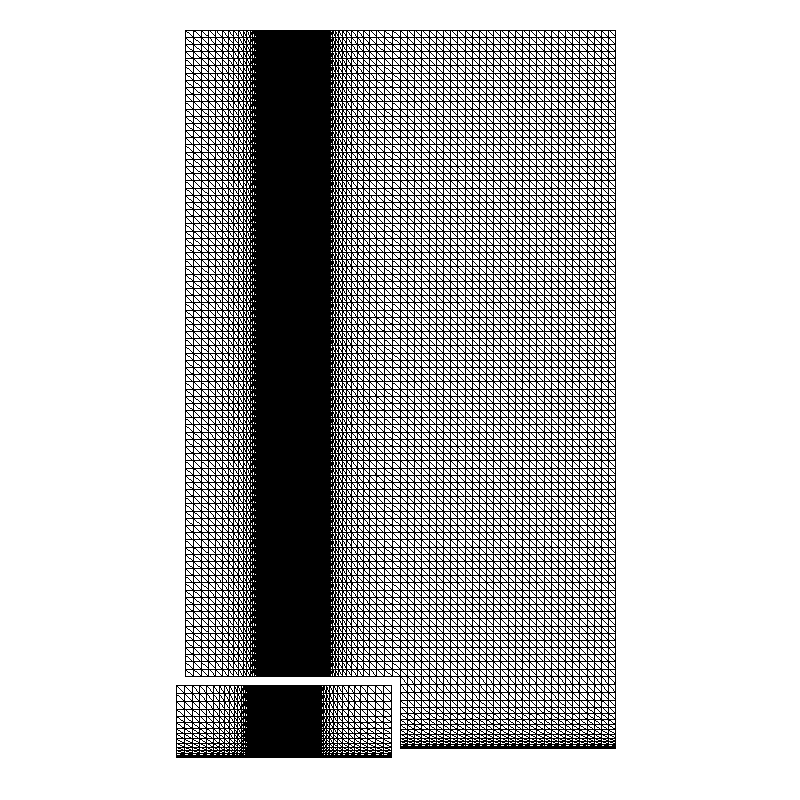
\includegraphics[width=\hsize, bb=0 0 800 800]{./img/ect_2d/mesh.png}
 \end{center}
 \caption{��¦�ˤ����Τ������Ĥ� 12 ����ͳ�٤��󼡸���å���}\label{fig:ect_2d_mesh}
\end{figure}
\begin{figure}[p]
 \begin{center}
  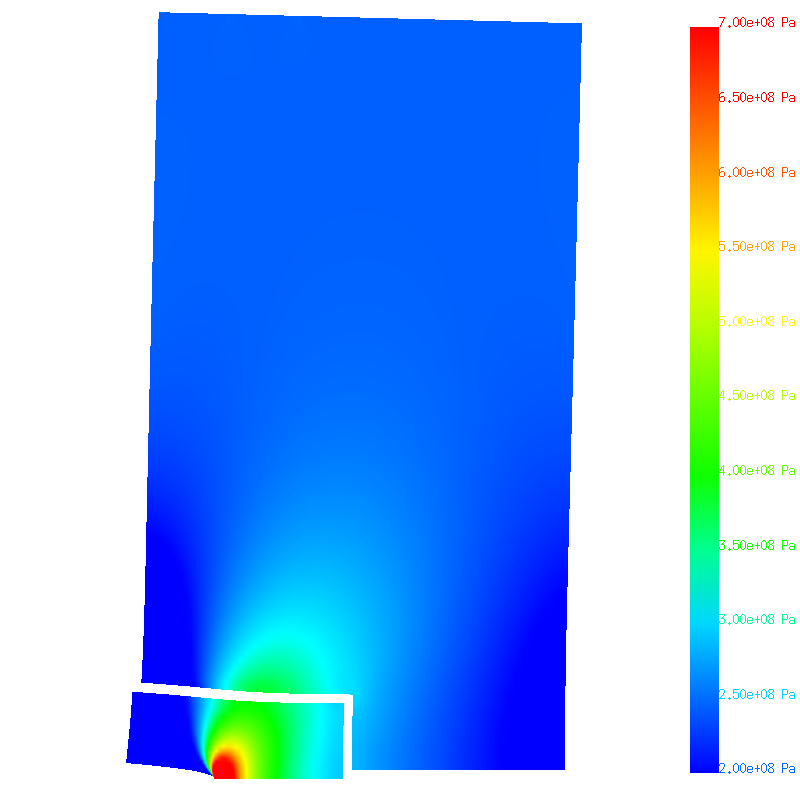
\includegraphics[width=\hsize, bb=0 0 800 800]{./img/ect_2d/result.png}
 \end{center}
 \caption{��¦�ˤ����Τ������Ĥ��󼡸����Ϸ�̤α��ϥ��󥿡��դ��ѷ���}\label{fig:ect_2d_result}
\end{figure}
\begin{figure}[p]
 \begin{center}
  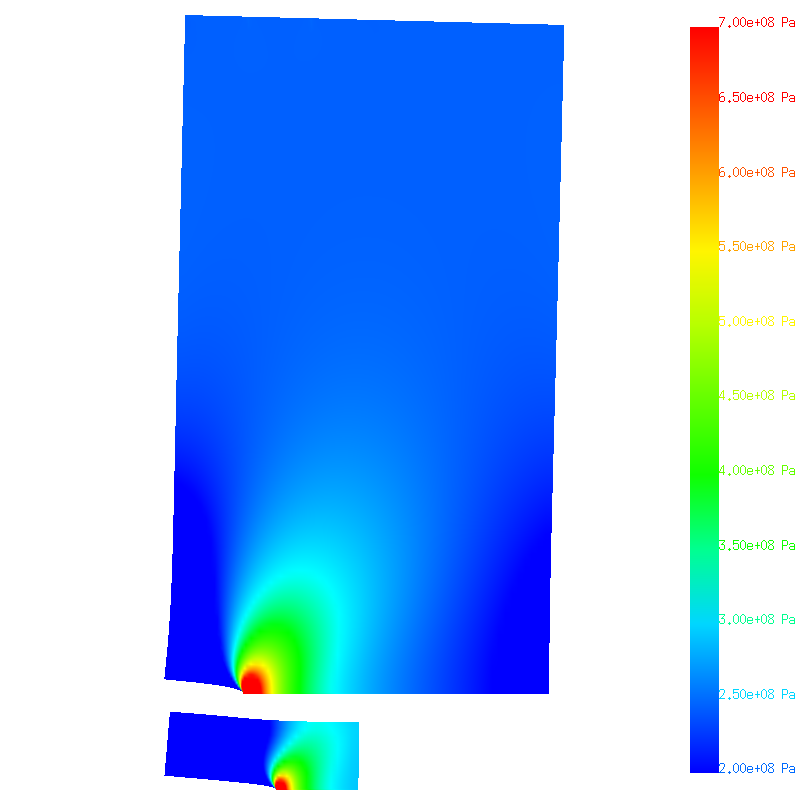
\includegraphics[width=\hsize, bb=0 0 800 800]{./img/ect_2d/result_zooming.png}
 \end{center}
 \caption{��¦�ˤ����Τ������ĤΥ����ߥ�ˡ�ˤ���󼡸����Ϸ�̤α��ϥ��󥿡��դ��ѷ���}\label{fig:ect_2d_result_zooming}
\end{figure}
\begin{figure}[p]
 \begin{center}
  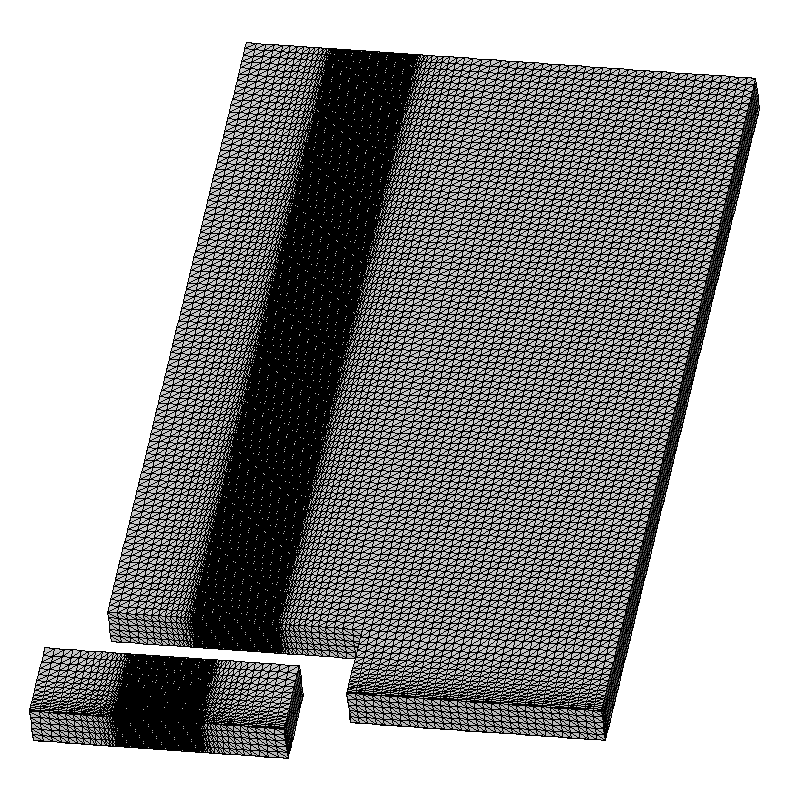
\includegraphics[width=\hsize, bb=0 0 800 800]{./img/ect_3d/mesh.png}
 \end{center}
 \caption{��¦�ˤ����Τ������Ĥ� 196 ����ͳ�٤λ�������å���}\label{fig:ect_3d_mesh}
\end{figure}
\begin{figure}[p]
 \begin{center}
  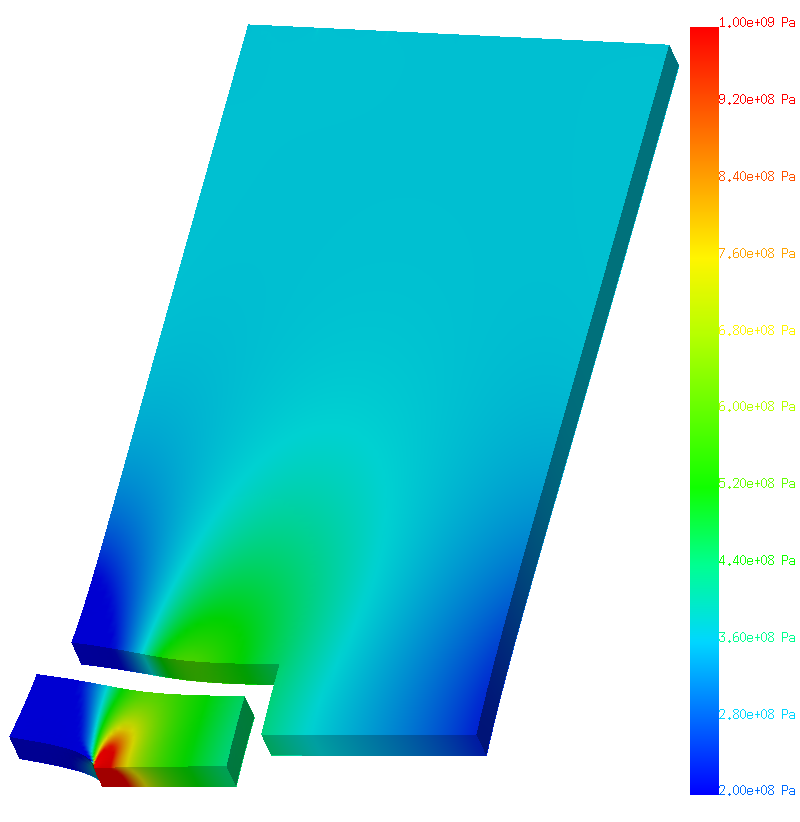
\includegraphics[width=\hsize, bb=0 0 800 800]{./img/ect_3d/result.png}
 \end{center}
 \caption{��¦�ˤ����Τ������Ĥλ��������Ϸ�̤α��ϥ��󥿡��դ��ѷ���}\label{fig:ect_3d_result}
\end{figure}

%% -*- coding: euc-jp -*-
\chapter{����}
�� 1 �ϤǤϡ��ܸ�����طʤ������Ū�ˤĤ��ƽҤ٤���

�� 2 �ϤǤϡ�
�ܸ�����طʤǤ����˲��ϳؤ���������Ӳ��Ϥγ��פˤĤ�������������
���ξϤǤϡ�
�ܸ���Υ������åȤǤ����絬���˲��ϳ�������Ф��뻰�Ĥδ�¸�δ�¸��ˡ�Ȥ��ơ�
�̾��ͭ�����Dz��Ϥ�Ԥ���ˡ�������ߥ�ˡ���Ź��å���ˡ�λ��Ĥ򼨤�����

�� 3 �ϤǤϡ�
�ޥ���ե����å���Ϣ�����Ϥ����Ϣ�����ϼ�ˡ�γ��פˤĤ��ƽҤ٤���
�ä�ʬΥȿ����ˡ�ˤĤ��ƽ���Ū�˽Ҥ٤���
�����ơ��絬���˲��ϳ�������Ф����¸��ˡ��Ϣ�����Ϥ����Ȥߤ�ʬ�ष����

�� 4 �ϤǤϡ�
�絬���˲��ϳ������ʬΥȿ��Ϣ����ˡ����Ѥ���Ȥ��Υ��르�ꥺ��ȼ����ˤĤ��ƽҤ٤���
�ܸ���Ǥ�ʬΥȿ��Ϣ����ˡ�Ȥ��� Aitken �䳰�ˤ��ưŪ�����դ��Υ֥��å� Gauss--Seidel ˡ���Ѥ�����
�ޤ���
���ξϤǤϥ������Х��ΰ褪��ӥ��������ΰ���ΰ襽��С��μ����ˤĤ��Ƥ�����������
�ܸ���Ǥ��ΰ襽��С��������������С��� LDL ʬ��ˡ���Ѥ�����

�� 5 �ϤǤϡ�
ʬΥȿ��Ϣ����ˡ���Ѥ��ƿ��ͼ¸���Ԥä���
�ޤ���ñ��ʷ����Υ�ǥ���Ѥ������������Ϥ��̤��ơ�
ʬΥȿ��Ϣ����ˡ��ȿ�������ˤĤ���Ĵ�١�
������·����伫ͳ�ٿ��˴ؤ�餺�ۤܰ����ȿ������Ǽ�«���뤳�Ȥ��狼�ä���
³���ơ��󼡸�����ӻ���������ϫ������Ÿ���Ϥ�Ԥä���
�󼡸��� 12 ����ͳ�٤β�����Ǥ��̾��ͭ������ˡ���� 12.9 �ܡ�
�������� 196 ����ͳ�٤β�����Ǥ� 4.52 �ܹ�®��������
�ޤ������٤��̾��ͭ������ˡ�Ȥۤ�Ʊ���Ǥ��ꡢ
�����ߥ�ˡ�Ȱ�ä����٤����������ΰ���礭���ˤۤȤ�ɰ�¸���ʤ����Ȥ��狼�ä���

����ʸ�Ǥϡ�
��ϫ������Ÿ����β�������̤��ơ�
�絬���˲��ϳ������ʬΥȿ��Ϣ����ˡ��Ŭ�Ѥ��뤳�Ȥ������򼨤�����
ʬΥȿ��Ϣ����ˡ���˲��ϳ���������ǤϤʤ���
���������ʤɤΤ�����ʣ�������ɽ�Ū��ȯ������褦��������̤�ͭ���Ǥ���ȹͤ����롣
�ʾ��դߤơ�
�����Ÿ˾����Ĥ��󤲤��롣
����ܤ϶ɽ�Ū������������ȯ�������̤�������ܼ�ˡ����Ѥ��뤳�ȤǤ��롣
�������䥯�꡼�פʤɤκ������������ݤ��ܿ��ʤɤζ������������ݤʤɡ�
�����ϳؤˤ������������ɽ�Ū��ȯ���������꤬¿����
����ʸ�Ǥ������˲��ϳ������ʬΥȿ��Ϣ����ˡ��Ŭ�Ѥ���������򼨤�������
���������ΰ褬��ʬ���Ϥ� Newton--Raphson ȿ����ȼ���褦������������ξ�硢
ʬΥȿ��Ϣ����ˡ�Υ��르�ꥺ��Υ롼�׹�¤���Ѳ����롣
���Τ褦������Ǥϡ�
ʬΥȿ��Ϣ����ˡ���Ѥ��뤳�Ȥ������˲��ϳ�������⤵��˸�ΨŪ�ʼ�����¸�ߤ���ȹͤ����롣
����ܤ�Ÿ˾�ϥ������Х��ΰ�Τ���ʤ��絬�ϲ��Ǥ��롣
����ʸ�Ǥ϶�ͭ����Ķ��ˤ����� 196 ����ͳ�٤λ�����������Ÿ���Ϥ򼨤�����
�����������ΤȤ��Υ������Х��ǥ�μ�ͳ�ٿ��ȥ��������ǥ�μ�ͳ�ٿ�������� 8:1 ���٤Ǥ��ä���
�ܼ�ˡ�Ϥ����椬�礭���ۤɸ�ΨŪ�ˤʤ뤳�Ȥ���¬����롣
����β�������⥰�����Х��ΰ�μ�ͳ�ٿ����礭���������Ϥ��뤿��ˤϡ�
�������̤����󤫤饹���ѡ�����ԥ塼���� PC ���饹�����Ѥ��뤳�Ȥ�ͭ���Ǥ��롣

%
%% acknowledgment
%% -*- coding: euc-jp -*-
\chapter*{�ռ�}
\mtcaddchapter[�ռ�]
����ʸ����������ر����طϸ���ʥ����ƥ��������칶�ν�����ʸ�Ȥ���Ʊ�칶�ε�¼���������漼�ˤ����ƺ������줿��ΤǤ���

��Ƴ���� (�纺) �Ǥ���Ʊ�칶�����ε�¼Ǧ���������Ѥ����äˤʤ�ޤ�����
��ر����ػ��˸����ϳؤ��μ�����̵���ä��䤬�׻��˲��ϳؤ˴ؤ��뽤����ʸ��ž夲�뤳�Ȥ��Ǥ����Τϵ�¼�����Τ������Ǥ���
�����򤪰������������������������������Ѹ���궵�����԰�͵��������ϵ��Ťʥ��ɥХ����򤤤������ޤ�����
Ʊ�칶�ڶ�������������������ϡ�
���漼�Υ��ߤˤơ�
��Ω����ˡ�͸����ؤ�Ĺ����̳�и��˴�Ť�����������ܤ��Ф��褦�ʰո����������������ޤ�����

Ʊ�칶������ƣ�潨������Ȥ� GNU/Linux �����Х���ե�� PC ���饹�����߷ס����ۤ˴ؤ��������Ԥ��ޤ�����
ƣ�椵��ˤϸ��漼�θ���ޥ͡����㡼�Ȥ��Ƥ�����Ū�ˤ����äˤʤ�ޤ�����
Ʊ�칶�������翦������꽨������ϡ�
�����¸��и���˳������˺������ٳؤˤĤ��ƶ����Ƥ��������ޤ�����
���ΰ���λҤ���ϻ�̳��³���ط������ˤ����ݤ򸫤Ƥ��������ޤ�����

��Ǥ������βϹ���֤���
���������Ĥ�����
��������Ҳ����󤵤�ˤϳز�ֱ���ʸ�ζ����ԤȤ��Ƥ����äˤʤꡢ
Ʊ����ľ��Ū�ʻ�Ƴ��¿�����������ޤ�����
�Ϲ礵�󤫤��ͭ������ˡ����ӷ׻����ϡ��ɥ�������
��󤫤�Ͽ�����������������������������ˡ��
�Ҳ����󤫤��ή�Ρ���¤Ϣ�����Ϥ��Ѥ������ˡ�ˤĤ��Ƽ�˶����ޤ�����
��Ǥ������ο��ܿ���Ϻ����ϡ�
NIS��NFS ���Τ�ʤ��ä���˥����д�����Ϣ���μ�������Ƥ��������ޤ�����
���ܤ��󤫤�ϼ��졦��¤Ϣ�����Ϥζ����ⶵ���Ƥ��������ޤ�����
������μ�ë��ʿ���󤫤�ϱ��ѿ����λ�������αԤ���Ŧ��¿�����������ޤ�����
������ҥ��󥵥��ȵ��ѳ�ȯ�����䷰���󤫤�� CAE (Computer-aided Engineering) �ζ����򶵤��ޤ�����

���漼��Ʊ�������ı������ˤ�����Ū�ˤȤƤ⤪���äˤʤ�ޤ�����
���ķ���ͥ���Ǽ�ݤ��ɤ��ΤǸ��漼�μ�Υ��٥�ȤǤϽ�����ޤ�����
���漼�θ��ڤ� Chi Wang ������¼�����������İ������������ͷ����ܺ���������
ͧ���ƻַ�������ε�췯����ܵ��׷�������ľ�з�����Է��ȤϿ������ä򤷤ޤ�����
��¼���Ȥ� SSH (Secure Shell) �ˤĤ��Ƹ��ޤ�����
���ķ��Ȥ� Git �ˤĤ��Ƹ��ޤ�����
�ܺ귯�Ȥ� Python �ˤĤ��Ƹ��ޤ�����
ͧ�����Ȥϥ����륹����ץȤˤĤ��Ƹ��ޤ�����
���ܷ��Ȥ� \LaTeX �ˤĤ��Ƹ��ޤ�����
����Ȥ� Emacs Lisp �ˤĤ��Ƹ��ޤ�����

%
%% references
%% -*- coding: euc-jp -*-
%% ����ʸ��
\begin{thebibliography}{99}
 \bibitem{ADVENTURE}
         ADVENTURE Project. \\
         \url{http://adventure.sys.t.u-tokyo.ac.jp/}
 \bibitem{Boeing787}
         Boeing 787 Dreamliner. \\
         \url{http://www.boeing.com/commercial/787family/}
 \bibitem{Davis2006}
         {\sc Davis, T. A.}
         {\it Direct Methods for Sparse Linear Systems}.
         Society for Industrial and Applied Mathematics, 2006.
 \bibitem{Farhat1991}
         {\sc Farhat, C. and Roux, F.-X.}
         A method of finite element tearing and interconnecting
         and its parallel solution algorithm.
         {\it International Journal for Numerical Methods in Engineering},
         vol.~32, issue~6, pp.~1205--1227, 1991.
 \bibitem{Fish1992}
         {\sc Fish, J.}
         The s-version of the finite element method.
         {\it Computers and Structures},
         vol.~43, issue~3, pp.~539--547, 1992.
 \bibitem{Intel_Compilers}
         Intel Compilers from Intel. \\
         \url{http://software.intel.com/en-us/articles/intel-compilers/}
 \bibitem{Kawai2006}
         {\sc Kawai, H.}
         ADVENTURE AutoGL:~a handy graphics and GUI library
         for researchers and developers of numerical simulations.
         {\it Computer Modeling in Engineering and Sciences},
         vol.~11, issue~3, pp.~111--120, 2006.
 \bibitem{Kelley2003}
         {\sc Kelley, C. T.}
         {\it Solving Nonlinear Equations with Newton's Method}.
         Society for Industrial and Applied Mathematics, 2003.
 \bibitem{Kikuchi2008}
         {\sc Kikuchi, M., Wada, Y., Takahashi, M. and Li, Y.}
         Fatigue crack growth simulation using s-version FEM.\
         {\it Advanced Materials Research},
         vols.~33--37, pp.~133--138, 2008.
 \bibitem{Mandel1993}
         {\sc Mandel, J.}
         Balancing domain decomposition.
         {\it Communications in Numerical Methods in Engineering},
         vol.~9, issue~3, pp.~233--241, 1993.
 \bibitem{Intel_MKL}
         Math Kernel Library from Intel. \\
         \url{http://software.intel.com/en-us/articles/intel-mkl/}
 \bibitem{Matthies2003}
         {\sc Matthies, H. and Steindorf, J.}
         Partitioned strong coupling algorithms
         for fluid--structure interaction.
         {\it Computers and Structures},
         vol.~81, pp.~805--812, 2003.
 \bibitem{Minami2010}
         {\sc Minami, S. and Yoshimura, S.}
         Performance evaluation of nonlinear algorithms with line-search
         for partitioned coupling techniques for fluid--structure interactions.
         {\it International Journal for Numerical Methods in Fluids},
         vol.~64, issues~10--12, pp.~1129--1147, 2010.
 \bibitem{Nagashima2003}
         {\sc Nagashima, T., Omoto, Y. and Tani, S.}
         Stress intensity factor analysis of interface cracks using X-FEM.\
         {\it International Journal for Numerical Methods in Engineering},
         vol.~56, issue~8, pp.~1151--1173, 2003.
 \bibitem{Nishikawa2007}
         {\sc Nishikawa, H., Serizawa, H. and Murakawa, H.}
         Actual application of FEM to analysis
         of large scale mechanical problems in welding.
         {\it Science and Technology of Welding and Joining},
         vol.~12, issue~2, pp.~147--152, 2007.
 \bibitem{Nishioka1983}
         {\sc Nishioka, T. and Atluri, S. N.}
         Analytical solution for embedded elliptical cracks,
         and finite element alternating method
         for elliptical surface cracks, subjected to arbitrary loadings.
         {\it Engineering Fracture Mechanics},
         vol.~17, issue~3, pp.~247--268, 1983.
 \bibitem{Ogino2005}
         {\sc Ogino, M., Shioya, R., Kawai, H. and Yoshimura, S.}
         Seismic response analysis of nuclear pressure vessel model
         with ADVENTURE system on the Earth Simulator.
         {\it Journal of the Earth Simulator},
         vol.~2, pp.~41--54, 2005.
 \bibitem{Okada2005}
         {\sc Okada, H. and Kamibeppu, T.}
         A virtual crack closure-integral method (VCCM)
         for three-dimensional crack problems
         using linear tetrahedral finite elements.
         {\it International Journal for Computational Methods
         in Engineering Science and Mechanics},
         vol.~10, issue~3, pp.~229--238, 2005.
 \bibitem{Okada2008}
         {\sc Okada, H., Kawai, H. and Araki, K.}
         A virtual crack closure-integral method (VCCM)
         to compute the energy release rates and stress intensity factors
         based on quadratic tetrahedral finite elements.
         {\it Engineering Fracture Mechanics},
         vol.~75, issue~15, pp.~4466--4485, 2008.
 \bibitem{Saad2003}
         {\sc Saad, Y.}
         {\em Iterative Methods for Sparse Linear Systems, Second Edition}.
         Society for Industrial and Applied Mathematics, 2003.
 \bibitem{Schenka2001}
         {\sc Schenka, O., G\"artnerb, K., Fichtnera, W. and Strickera, A.}
         PARDISO:~a high-performance serial and parallel sparse linear solver
         in semiconductor device simulation.
         {\it Future Generation Computer Systems},
         vol.~18, issue~1, pp.~69--78, 2001.
 \bibitem{Sugimoto2010}
         {\sc Sugimoto, S., Margron, V. and Yoshimura, S.}
         Parallel vibration analysis of magnetic--structural coupled phenomena
         of MRI model.
         In {\it Proceedings
         of the 9th World Congress on Computational Mechanics
         and the 4th Asian Pacific Congress on Computational Mechanics},
         Sydney, Australia, July 2010.
 \bibitem{Terada2001}
         {\sc Terada, K. and Kikuchi, N.}
         A class of general algorithms for multi-scale analyses
         of heterogeneous media.
         {\it Computer Methods in Applied Mechanics and Engineering},
         vol.~190, issues~40--41, pp.~5427--5464, 2001.
 \bibitem{Tezduyar2007}
         {\sc Tezduyar, T. E. and Sathe, S.}
         Modelling of fluid--structure interactions
         with the space--time finite elements: solution techniques.
         {\it International Journal for Numerical Methods in Fluids},
         vol.~54, issues~6--8, pp.~855--900, 2007.
 \bibitem{Yagawa1991}
         {\sc Yagawa, G., Soneda, N. and Yoshimura, S.}
         A large scale finite element analysis
         using domain decomposition method on a parallel computer.
         {\it Computers and Structures},
         vol.~38, issues~5--6, pp.~615--625, 1991.
 \bibitem{Yagawa1993}
         {\sc Yagawa, G., Yoshioka, A., Yoshimura, S. and Soneda, N.}
         A parallel finite element method with a supercomputer network.
         {\it Computers and Structures},
         vol.~47, issue~3, pp.~407--418, 1993.
 \bibitem{Yagawa1993_2}
         {\sc Yagawa, G. and Shioya, R.}
         Parallel finite elements on a massively parallel computer
         with domain decomposition.
         {\it Computing Systems in Engineering},
         vol.~4, issues~4--6, pp.~495--503, 1993.
 \bibitem{Yamada2011}
         {\sc Yamada, Takahiro.}
         Finite element procedure for overlapping meshes
         based on domain decomposition approach using background voxel mesh.
         In {\it Proceedings of the 11th US National Congress
         on Computational Mechanics},
         213901, Minneapolis, MN, USA, July 2011.
 \bibitem{Yamada2008}
         {\sc Yamada, Tomonori and Yoshimura, S.}
         Line search partitioned approach
         for fluid--structure interaction analysis of flapping wing.
         {\it Computer Modeling in Engineering and Sciences},
         vol.~24, issue~1, pp.~51--60, 2008.
 \bibitem{Yoshimura2002}
         {\sc Yoshimura, S., Shioya, R., Noguchi, H. and Miyamura, T.}
         Advanced general-purpose computational mechanics system
         for large-scale analysis and design.
         {\it Journal of Computational and Applied Mathematics},
         vol.~149, issue~1, pp.~279--296, 2002.
 \bibitem{Zhang2001}
         {\sc Zhang, Q. and Hisada, T.}
         Analysis of fluid--structure interaction problems
         with structural buckling and large domain changes
         by ALE finite element method.
         {\it Computer Methods in Applied Mechanics and Engineering},
         vol.~190, issue~48, pp.~6341--6357, 2001.
 \bibitem{Oguni1991}
         {\sc ������ ����, ¼�ķ�Ϻ, ������Ϻ, Dongarra, J. J., Ĺë�ɧ ��.}
         ����׻����եȥ�����---WS�������ѡ���������׻���.
         ����, 1991.
 \bibitem{shippai}
         �����μ��ǡ����١���. \\
         \url{http://www.sozogaku.com/fkd/}
 \bibitem{Shiratori1980}
         ��Ļ����, ������Ϻ, ������ͺ ����.
         �����˲��ϳ�.
         �¶�����, 1980.
 \bibitem{Suzuki1999}
         ���ڹ, ���ڱѿ�, �ܾ���, �������Ϻ.
         �Ź��å���ˡ�ˤ�����ι�¤�Υޥ�������������.
         {\it Transactions of the Japan Society
         for Computational Engineering and Science},
         vol.~1999, 19990020, 1999.
 \bibitem{Suzuki2002}
         ���ڹ, ���ڱѿ�, �潻����, ��¼��μ.
         �Ź��å���ˡ�ˤ����륰�����Х롦��������ȿ������.
         ����¤���ز���ʸ��,
         vol.~192, pp.~691--696, 2002.
 \bibitem{jsmecode}
         ���ܵ����ز�.
         ȯ���Ѹ������������ʰݻ����� (JSME S NA1-2004),
         2004.
 \bibitem{Yagawa1988}
         ����� ��.
         �˲��ϳ�---���������Ϥ��鹩��Ū���Ѥޤ�.
         ������, 1998.
\end{thebibliography}

%
%% appendix
% \appendix
% \include{appendix}
%
\end{document}
